%%==================================================
%% diss.tex for SJTU Master Thesis
%% based on CASthesis
%% modified by wei.jianwen@gmail.com
%% version: 0.3a
%% Encoding: UTF-8
%% last update: Dec 5th, 2010
%%==================================================

% 字号选项: c5size 五号(默认) cs4size 小四
% 双面打印(注意字号设置)
\documentclass[cs4size, a4paper, twoside]{sjtuthesis}
% 单面打印(注意字号设置)
% \documentclass[cs4size, a4paer, oneside, openany]{sjtuthesis}


\usepackage{algorithm}               %format of the algorithm
\usepackage{algorithmic}             %format of the algorithm
\usepackage{multirow}                %multirow for format of table
\usepackage{amsmath}
\usepackage{amsfonts}

\usepackage{mathrsfs}

\usepackage{listings}
\usepackage{float}

\renewcommand{\algorithmicrequire}{\textbf{Input:}}
\renewcommand{\algorithmicensure}{\textbf{Steps:}}
\renewcommand{\algorithmiccomment}[1]{// #1}

% \usepackage[sectionbib]{chapterbib}%每章都用参考文献

\newboolean{DOIT}
\setboolean{DOIT}{false}%编译某些只想自己看的内容,编译true,否则false

%% 行距缩放因子(x倍字号)
\renewcommand{\baselinestretch}{1.3}

% 设置图形文件的搜索路径
\graphicspath{{figure/}{figures/}{logo/}{logos/}{graph/}{graphs}}

%%========================================
%% 在sjtuthesis.cls中定义的有用命令
%%========================================
% \cndash 中文破折号
% 数学常量
% \me 对数常数e
% \mi 虚数单位i
% \mj 虚数单位j
% \dif 直立的微分算符d为直立体。
% 可伸长的数学箭头、等号
% \myRightarrow{}{}
% \myLeftarrow{}{}
% \myBioarrow{}{}
% \myLongEqual{}{}
% 参考文献
% \upcite{} 上标引用
%%========================================


\begin{document}

%%%%%%%%%%%%%%%%%%%%%%%%%%%%%%
%% 封面
%%%%%%%%%%%%%%%%%%%%%%%%%%%%%%

% 中文封面内容(关注内容而不是形式)
\title{同义词搜索和抗信息泄漏的对称可搜索加密技术的研究}%对称可搜索加密技术的若干问题研究
\author{柳祚鹏}
\advisor{丁宁}
\degree{硕士}
\defenddate{2015年1月16日}
\school{上海交通大学}
\institute{电子信息与电气工程学院}
\studentnumber{1120339063}
\major{计算机科学与技术}



% 英文封面内容(关注内容而不是表现形式)
\englishtitle{Research on synonym search and leakage-resilient in SSE}
\englishauthor{\textsc{Zuopeng Liu}}
\englishadvisor{Prof. \textsc{Ning Ding}}
\englishschool{Shanghai Jiao Tong University}
\englishinstitute{\textsc{Depart of Computer Science and Engineering, School of Electronic Information and Electrical Engineering} \\
  \textsc{Shanghai Jiao Tong University} \\
  \textsc{Shanghai, P.R.China}}
\englishdegree{Master}
\englishmajor{Computer Science and Technology}
\englishdate{Jan. 16th, 2015}





% 封面
\maketitle

% 英文封面
\makeenglishtitle

% 论文原创性声明和使用授权
\makeDeclareOriginal
\makeDeclareAuthorization

%%%%%%%%%%%%%%%%%%%%%%%%%%%%%%
%% 前言
%%%%%%%%%%%%%%%%%%%%%%%%%%%%%%
\frontmatter

% 摘要
%%==================================================
%% abstract.tex for SJTU Master Thesis
%% based on CASthesis
%% modified by wei.jianwen@gmail.com
%% version: 0.3a
%% Encoding: UTF-8
%% last update: Dec 5th, 2010
%%==================================================

\begin{abstract}

  在大数据时代,越来越多的用户开始使用廉价和计算能力强大的云外包服务。然而安全因素成为了它进一步发展的主要障碍,导致该问题的原因在于:云外包商并非完全可信,致使远程外包的数据处在危险之中。一个简单的解决方案是在数据外包之前对数据加密。但是,加密限制了用户对数据的有效检索。为此,如何避免云端数据被未经授权的人所访问并维持对加密数据的有效计算,已成为云计算外包领域的研究重点。

  基于安全索引的可搜索加密技术解决了该难题。可搜索加密技术主要包括:对称可搜索加密技术、公钥可搜索加密技术和隐私信息检索,它们分别解决了不同场景下的应用难题。本文仅仅关注云计算环境下的对称可搜索加密技术,其主要研究内容是对称云环境下的隐私泄漏问题和复杂条件搜索的情形。

  为了弥补Non-adaptive安全模型中信息泄漏过多的缺陷,我们基于史密斯正交化理论提出了一个以概率抗信息泄漏的方案。与已有的可搜索加密方案相比,我们的方案在减少信息泄漏的同时,并且没有增加客户端的计算与存储开销以及双方交互的通讯开销,同时达到了相同的安全级别。不幸的是,方案提高了服务器的存储和计算开销。通过在安全和性能之间权衡,我们证明这个代价是可取的,并且使方案获得了良好的可扩展性。

  另外,到目前为止,没有一个方案对复杂条件搜索下的同义词搜索问题进行研究。在用户记忆具有有限性和人员频繁变更的场景下,以前的方案显得有些难以应付,于是我们认真地研究了该问题。紧接着,我们设计了一个支持同义词搜索的方案。该方案有如下优势:我们第一次阐述了同义词可搜索问题;我们引入了同义词函数和同义词集合,增加了方案的可扩展性;并且通过严格的安全分析,证明我们提出的方案是正确的和Non-adaptive安全的。此外,我们提出的算法是高效的,它没有增加用户的计算和存储开销,传输开销仍为$O(1)$,查找时间复杂度仅为$O(p)$($p$ --- 单词同义词集合的最大长度)。通过返回所有同义词的文档集合,该技术大大克服了已有方案的不足 --- 模糊搜索不能解决所有相似搜索问题,提高了系统的可适用性。因而,我们提出的方案是非常实用的并且弥补了理论与现实的差距。





  %%对称可搜索加密技术允许用户外包加密的数据至不可信的云服务提供商,并维持用关键字进行有效检索的能力。
%%
%%  随着云计算的飞速发展,越来越多的用户将敏感数据集中存放到云服务端,以避免繁琐的本地管理并获取更多便捷的服务。与此同时由于云服务提供商并非完全可信,如何保证云端数据的隐私--- 即如何避免云端数据被未经授权的人所访问已成为云计算环境下安全隐私问题的研究重点。为此,一项新的研究技术 --- " 云计算环境下的可搜索加密技术" 解决了此难题。 一些学者率先提出了“云计算环境下的可搜索加密技术”的研究课题。可搜索对称加密技术即用户将数据加密存储到服务端,同时服务端维持对加密数据进行有效检索的能力。
%%
%%  本课题研究重点是:对称可搜索加密技术(可搜索加密技术主要包括:对称可搜索加密技术、公钥可搜索加密技术和隐私信息检索)中模糊对称可搜索加密和动态可搜索加密技术。文中首先分析了现有方案的研究状况;然后找出现有方案中存在的不足和被忽略的问题;最后通过解决原有方案中存在的潜在问题和扩充原有模糊方案的功能—支持语义搜索,提出一种更实用、更高效、功能更强大并且没有降低安全性能的新方案,使之尽可能支持动态和模糊功能并且没有增加信息泄露。


  \keywords{\large 可搜索加密 \quad 同义词搜索 \quad 信息泄漏 \quad 搜索模式 \quad 访问模式 }
\end{abstract}

\begin{englishabstract}


  In an era of mass data, more and more users start to utilize cloud outsourcing services of cheap and powerful computing ability. While security problem has become a main obstacle to its further moveforward. The fact that the cloud server provider is "honest-but-curious" might make outsourced data at risk. A naive method is that these data have to be encrypted prior to outsource to the remote semi-trusted servers to combating unsolicited accesses. But unfortunately, encrypted data restricts the users' effective search ability. Therefore, this point that how to avoid accessing the outsourced data by unauthorized users while maintaining effective computing on encrypted data has been closely researched in the field of cloud outsourcing.

  The searchable encryption technique based on secure index, which has been a key and lead solution, solves this issue. It mainly consists of symmetric searchable encryption (SSE), public-key searchable encryption (PKSE) and private information retrieval (PIR). And they, respectively, work out the problem of application under different scenarios. In this thesis, we only focus on SSE technique in the context of cloud computing.The dissertation concerns about researching on problems of data privacy leakage and complexity search on encrypted data in untrusted cloud setting.

  In order to make up the defects of information leakage of Non-adaptive security model in the phrase of query, we based on the smith orthogonalization theory present a scheme of resisting leakage of trace in probability. Compared with the previous single keyword search works, not only does our solution leak less information, but also it doesn't increase the computing and storage overheads of clients and communication cost in the mutual interactive process. It is unfortunate that this scheme greatly improves the storage and computational overhead of servers. At last, by balancing trade-off between security and capability, we show that it is desirable to increase this cost and extends scalability and usability of our solution in practice.

  In addition, there exists no such solution focusing on the synonym search in the setting of complexity search. In consideration of finiteness of people's memory and people's frequent changing, existing schemes seem to be difficult to deal with this case. To this case, we seriously study this issue. Soon afterwards, we firstly design a formal Practical Synonym Symmetric Searchable Encryption Solution (PSSSE) in this thesis. Our proposed technique have a number of crucial advantages. To our best knowledge, we for the first time put forward the issue of the synonym keyword search over remotely encrypted data in the context of cloud computing. In this scheme, we introduce the concepts of synonym function and synonym sets to obtain better scalability. Through rigorous security analysis, we show that our proposed solution is correct and privacy-preserving (non-adaptive security) without the loss of function of the scheme. Besides, the algorithms we present are simple and effective, it almost increases no space and computing overhead of the user. The overhead of communication still remains $O(1)$. The time complexity of searching on encryption data is $O(p)$ ($p$ --- the maximum number of synonym of keyword). This scheme greatly enhances system's usability by responding all documents containing keyword and corresponding synonyms. Hence, our solution is very significant to practical use and bridges the gap of state-of-art.
 %% In addition, there exists no such solution focusing on the synonym search in the setting of complexity search. In consideration of finiteness of people's memory and lifetime of people's knowledge, we seriously study this issue. In this paper, we design a scheme for the problem of synonym search, and provide the proof of security. Our proposed technique have a number of crucial advantages. We for the first time put forward the problem of the synonym keyword search over remotely encrypted data in the context of cloud computing. In our scheme, we introduce the concepts of synonym function and synonym sets. We firstly implement a formal practical Synonym Symmetric Searchable Encryption Solution (PSSSE). Through rigorous security analysis, we show that our proposed solution is correct and privacy-preserving (non-adaptive security) without the loss of function of the scheme. Besides, the algorithms we present are simple and effective, it almost increases no space and computing overhead of the user. The overhead of communication still remains $O(1)$. The time complexity of searching on encryption data is $O(p)$ (p --- the maximum number of synonym of keyword). To apply to general situation, we simultaneously give a practical trade-off between availability and performance. This scheme greatly enhances system usability by responding the answers that are all documents containing keyword and corresponding synonyms. Hence, our solution is very significative to practical use and bridges the gap of state-of-art.

%%An imperial edict issued in 1896 by Emperor Guangxu, established Nanyang Public School in Shanghai. The normal school, school of foreign studies, middle school and a high school were established. Sheng Xuanhuai, the person responsible for proposing the idea to the emperor, became the first president and is regarded as the founder of the university.
%%
%%During the 1930s, the university gained a reputation of nurturing top engineers. After the foundation of People's Republic, some faculties were transferred to other universities. A significant amount of its faculty were sent in 1956, by the national government, to Xi'an to help build up Xi'an Jiao Tong University in western China. Afterwards, the school was officially renamed Shanghai Jiao Tong University.
%%
%%Since the reform and opening up policy in China, SJTU has taken the lead in management reform of institutions for higher education, regaining its vigor and vitality with an unprecedented momentum of growth. SJTU includes five beautiful campuses, Xuhui, Minhang, Luwan Qibao, and Fahua, taking up an area of about 3,225,833 m2. A number of disciplines have been advancing towards the top echelon internationally, and a batch of burgeoning branches of learning have taken an important position domestically.
%%
%%Today SJTU has 31 schools (departments), 63 undergraduate programs, 250 masters-degree programs, 203 Ph.D. programs, 28 post-doctorate programs, and 11 state key laboratories and national engineering research centers.
%%
%%SJTU boasts a large number of famous scientists and professors, including 35 academics of the Academy of Sciences and Academy of Engineering, 95 accredited professors and chair professors of the "Cheung Kong Scholars Program" and more than 2,000 professors and associate professors.
%%
%%Its total enrollment of students amounts to 35,929, of which 1,564 are international students. There are 16,802 undergraduates, and 17,563 masters and Ph.D. candidates. After more than a century of operation, Jiao Tong University has inherited the old tradition of "high starting points, solid foundation, strict requirements and extensive practice." Students from SJTU have won top prizes in various competitions, including ACM International Collegiate Programming Contest, International Mathematical Contest in Modeling and Electronics Design Contests. Famous alumni include Jiang Zemin, Lu Dingyi, Ding Guangen, Wang Daohan, Qian Xuesen, Wu Wenjun, Zou Taofen, Mao Yisheng, Cai Er, Huang Yanpei, Shao Lizi, Wang An and many more. More than 200 of the academics of the Chinese Academy of Sciences and Chinese Academy of Engineering are alumni of Jiao Tong University.
%%

  \englishkeywords{\large searchable encryption, synonym search, information leakage, search pattern, access pattern}
\end{englishabstract}


% 目录
\tableofcontents
% 表格索引
\listoftables
% 插图索引
\listoffigures

\addcontentsline{toc}{chapter}{\listfigurename} %将表格索引加入全文目录
\addcontentsline{toc}{chapter}{\listtablename}  %将图索引加入全文目录

% 主要符号、缩略词对照表
%%%==================================================
%% symbol.tex for SJTU Master Thesis
%% based on CASthesis
%% modified by wei.jianwen@gmail.com
%% version: 0.3a
%% Encoding: UTF-8
%% last update: Dec 5th, 2010
%%==================================================

\chapter{主要符号对照表}
\label{chap:symb}
\begin{tabular}{ll}

 \hspace{2em}$\epsilon$       & \hspace{5em}介电常数 \\
 \hspace{2em}$\mu$ \qquad     & \hspace{5em}磁导率 \\
  \hspace{2em}$\epsilon$       & \hspace{5em}介电常数 \\
 \hspace{2em}$\mu$ \qquad     & \hspace{5em}磁导率 \\
 \hspace{2em}$\epsilon$       & \hspace{5em}介电常数 \\
 \hspace{2em}$\mu$ \qquad     & \hspace{5em}磁导率 \\
 \hspace{2em}$\epsilon$       & \hspace{5em}介电常数 \\
 \hspace{2em}$\mu$ \qquad     & \hspace{5em}磁导率 \\


\end{tabular}


%%%%%%%%%%%%%%%%%%%%%%%%%%%%%%
%% 正文
%%%%%%%%%%%%%%%%%%%%%%%%%%%%%%
\mainmatter


%% 各章正文内容
%%==========================
%% chapter01.tex for SJTU Master Thesis
%% based on CASthesis
%% modified by wei.jianwen@gmail.com
%% version: 0.3a
%% Encoding: UTF-8
%% last update: Dec 5th, 2010
%%==================================================

%\bibliographystyle{sjtu2} %[此处用于每章都生产参考文献]
%%%%%%%%%%%%%%%%%%%%%%%%%%%%%%%%%%%%%%%%%%%%%%%%%%%%%
%%
%%   绪论
%%
%%%%%%%%%%%%%%%%%%%%%%%%%%%%%%%%%%%%%%%%%%%%%%%%%%%%%
\chapter{绪论}
\label{chap:introduction}

%%%%%这是上海交通大学(非官方)硕士学位学位论文 \LaTeX 模板,当前版本是 \version 。


%%%%%%%%%%%%%%%%%%%%%%%%%%%%%%%%%%%%%%%%%%%%%%%%%%%%%
%%
%%   研究背景和意义
%%
%%%%%%%%%%%%%%%%%%%%%%%%%%%%%%%%%%%%%%%%%%%%%%%%%%%%%
\section{研究背景及意义}
\label{sec:instroduction_background}

 随着网络技术的飞速发展,人们生活中的点点滴滴(从办公、娱乐到洗衣、做饭)逐渐网络化,导致网络中数据的量级呈指数增长。在这些数据的面前,先前的计算技术和存储能力显得有些力不从心。在此背景之下,一种全新的网络技术油然而生 --- 即“云存储”和“云计算”技术。它们的出现分别从理论上解决了大数据的存储和计算问题。为此,实际中各大企业纷纷提出不同场景下的“云”解决方案以满足各自的需求。亚马逊(Amazon)率先推出弹性计算云(Elastic Compute Cloud --- EC2)服务\cite{walker2008benchmarking};Google 首席执行官埃里克·施密特(Eric Schmidt)在搜索引擎大会首次提出“云计算”(Cloud Computing)\cite{bogatin2006google}的概念;随后包括IBM、Microsoft、Intel、Apple 和YAHOO等一些大型企业都开始部署自己的云存储和计算平台。由此,网络计算和存储的发展正式进入“云”的世界。

 “云计算”是一种基于互联网的计算方式,按照这种方式,云终端将已部署的资源(如网络、服务器、存储、应用及服务)按需提供给云用户,并最大程度地减少用户对资源的管理和配置\cite{mell2009nist}。通过互联网,云计算为使用者提供强大的可伸缩和廉价的分布式计算能力,并且在使用过程中,使用者不需要了解云端基础技术的细节和具备相关的专业知识,就能对云端资源进行合理的控制和使用。根据美国国家标准与技术研究院(NIST) 的定义\cite{above2009Armb},云计算提供三种不同层次的服务:
 \begin{enumerate}
   \item
   软件即服务(SaaS):用户可以通过租借云平台上的软件来为自己提供服务或无偿使用一些基础服务软件;

   \item
   平台即服务(PaaS):用户利用云计算服务提供商的平台,通过免费或低价租借的方式来部署自己的软件;

   \item
   基础设施即服务(IaaS):云用户可以利用云平台基础设施来获得所需服务。

 \end{enumerate}

 当前的云计算模型按照部署方式主要包括公有云、私有云、社群云和混合云。公有云通过网络及第三方服务提供给用户使用;私有云具有许多公有云环境下的优点(如弹性,实时提供服务),两者差别主要在于,私有云资源仅需在组织内部管理和使用,不会受到网络带宽和安全疑虑的影响;社群云主要由许多利益相仿的组织掌握和使用,社群内成员可以使用共有的资源,避免了公有云开放环境的安全问题;混合云则基于经济性、可用性等的考虑,是公有云和私有云的结合。云计算部署模型从数据隐私方面的角度来考虑,具备以下特点:
 \begin{itemize}
   \item
   在公有云环境下,由于数据拥有者与服务提供商站在不同的立场上并且拥有不同的利益,使得服务提供商并不被完全信任(semi-trusted);

   \item
   在私有云环境下,虽然云资源仅在组织内部使用,但由于云计算普遍采用虚拟化技术\cite{chiueh2005survey}来提高系统的资源利用率和降低运营成本,不同用户的数据可以同时在同一物理服务器上进行计算和存储。跨虚拟机攻击\cite{ristenpart2009hey} 使得用户数据有可能被同一物理服务器上的其他用户非授权访问。

 \end{itemize}

 由于“云”计算提供廉价的计算和强大的可伸缩,越来越多的用户将本地的数据移植到“云”平台。与此同时,一些云安全事故也频频发生(e.g.2011年谷歌邮箱爆发大规模的用户数据泄漏事件,2014年Apple公司icloud 帐号泄漏事件)。在透明的云环境下,用户简单地将数据以明文形式存储在云服务端存在明显的缺陷 --- 数据安全隐患。因此,当数据拥有者将数据存储到云服务端后,如何确保云端数据隐私,避免云端数据被未经授权用户所访问成为云端数据隐私安全研究的焦点。

%% 为了解决上述安全问题,最简单的做法就是用户在将其数据上传至非可信服务器之前,先进行数据加密;当需要使用数据时,从服务器下载密文数据并进行解密。这种做法在解决数据隐私性问题的同时,带来了新的数据可用性问题 --- 如何对服务器上的数据进行有效地搜索。由于数据处于加密状态,服务器无法解密,在传统安全机制下,云用户只能下载所有上传的数据,解密之后进行搜索。这种做法将耗费大量的网络资源,且并没有充分利用云端强大的计算能力。

%%为了解决上述查找低下的不足

为了解决该安全隐患带来的缺陷,一些学者利用传统的安全机制解决了数据隐私泄漏的问题,具体过程如下:数据拥有者在将数据存储到并非完全可信的服务端之前,首先将数据加密\cite{biham1993differential}, 然后将数据以密文的形式存储到云服务端;当用户需要使用数据时,首先将存储在服务器端的加密数据全部下载下来,然后进行解密并查找获得所需的文件。该机制虽然解决了数据的隐私问题,同时带来了新的问题 --- 如何才能保证云存储和计算资源被高效地利用。这种做法不仅耗费大量的网络资源,同时也增加了用户的计算开销,这些都与云计算服务的设计理念和用户需求相违背。因此,如何高效利用云端的存储和计算能力是当前关注的重点。

为了解决上述查找效率低下的缺陷,在“云”计算平台下一种新的确保数据隐私且具备高效计算的技术被提出 --- 可搜索加密技术。可搜索加密技术解决了上述难点,其过程描述如下:数据拥有者对文档进行可搜索加密,然后存储到云服务平台;当授权的用户需要查找文档时,使用搜索条件陷门(Trapdoor)生成算法将单词的陷门提交至云服务端;一旦云服务端收到搜索陷门后,便直接在用户的密文数据上进行搜索操作,并将搜索结果返回给用户。在方案整个过程中,云服务器无法知晓用户数据以及搜索条件的任何信息,保证了数据隐私性;在网络上仅传输符合搜索条件的数据,而不是所有外包的数据,大大降低了网络资源的消耗;同时请求者只需解密符合条件的文档,大大节省了用户昂贵的计算能力和存储空间。


可搜索加密技术包括对称可搜索加密(Symmetric searchable encryption)、公钥可搜索加密(Public key encryption with keyword search)和多用户(Multi-User)可搜索加密技术。近年来,这些技术都得到的广泛的关注。它们的研究领域极其广泛,包括:单关键字搜索、多关键字搜索、模糊搜索、范围搜索、布尔搜索搜索和动态搜索等。这些方案试图提供一个具有完备功能、高性能和强安全的解决方案。相似搜索(包括模糊搜索和同义词搜索\cite{grefenstette1994explorations})在明文场景下得到了广泛的研究和应用,虽然这些技术在加密数据上也被关注和研究,但是其研究成果尚有不足。并且在实际研究中,人们仅仅关注模糊搜索却忽略了同义词搜索的情形。此外,这些基于逆向索引的方案在查找时的信息泄漏有所偏多 --- 包括大小模式(size pattern)、访问模式(access pattern) 和搜索模式(search pattern),可以得到进一步的降低。

综上所述,我们能进一步对相似搜索技术进行的研究,不仅由于其方案不够完善同时包括原有方案存在缺陷;特别是同义词搜索技术,它在实际应用中也存在着极大的需求,因而提出安全的相似搜索加密方案对理论和实际都具有远大的意义。同样地,对目前基于semi-trusted的云环境下的对称可搜索的方案的信息泄漏问题进行深入研究,更多地保护用户的搜索隐私,即解决如何进一步降低这些信息的泄漏的问题,不仅能加快推进其在实际中应用的进度,同时也使可搜索加密技术在安全上有所突破,树立一个新的里程碑。为此,探究实用的相似可搜索方案和减少信息在云计算可搜索场景下的泄漏,对安全的云计算的普及具有重要的意义。


%%%对文件进行某种加密的对称可搜索加密技术在解决了上述问题的同时,带来了搜索效率的问题—如何避开对非结果文件进行搜索。为了解决上述暴露的搜索效率问题,一些学者在原有技术的基础上提出了新的解决方案-- 基于安全索引的可搜索加密技术。其基本过程如下:用户首先将文件中以单词为单位(反向索引)或文件为单位(正向索引)来构建安全索引,然后将安全索引和数据的密文形式(以某种加密算法加密)存储到云服务端;当用户需要查询包含某单词的文件时,用户首先计算该单词的令牌并将令牌发送给云服务端,然后云服务端使用单词令牌在安全索引上直接进行搜索,最后仅将满足搜索条件的结果返回给用户。在方案的整个过程中,文件以密文形式存储和服务器的搜索建立在安全索引上,没有暴露用户数据的任何明文信息给服务端,既保证了数据的隐私或由于在安全索引上进行搜索而导致少量的必要的信息泄漏(主要包括size pattern、access pattern 和搜索search pattern);同时仅返回查询结果,降低了网络的传输开销和用户的计算开销。


%%上述可搜索加密技术解决了数据外包带来的安全隐患,仅适用于精确搜索的情形—即用户输入单词即恰好为搜索单词的情形。但是在现实环境下,用户在查询时输入单词中可能包含少量错误(例如将“exact”写成了“egact”)或者输入格式不一致(例如将“data-mining”写成“data mining”),使得在上述精确的可搜索方案下无法进行有效搜索,为此需提供一种既能进行精确搜索又能容忍较小错误的搜索方案。在明文搜索环境下,容忍错误的搜索技术—模糊搜索使用了简单的单词拼写检查机制,这样方式虽然能从一定程度上解决该问题,但是存在以下两个主要的问题:用户需要进行交互并花费额外的计算开销来从拼写检查算法的候选单词集中确定正确的单词;同时当用户误输入某些有效的单词(如将“cat”写成“bat”)时,拼写检查算法失效。为了解决密文环境下的模糊搜索问题,一些学者[9]在前人成果上(精确可搜索加密技术、数据库模糊查询[20]以及明文模糊搜索技术)提出了技术解决方案— 基于编辑距离和通配符的模糊可搜索加密技术。其过程如下:用户首先对每个单词的模糊集构建安全索引,然后包含模糊信息的安全索引和数据密文存储到云服务端;在查询时,用户构建待查单词的模糊集并将模糊集生成的令牌集发送给服务端,最后在服务端的安全索引上进行搜索并返回查找的结果。该方案虽然解决了模糊可搜索加密的问题,同时存在一定不足之处—即在构建索引和查询时,对每个单词构建模糊集显然增加了服务端的存储开销和网络的传输代价以及用户的计算开销,同时不同单词的模糊集可能存在交集也将导致一定的信息泄漏。为此,能否构建一个更有效的和安全的模糊可搜索加密方案成为本课题研究的焦点。
%%
%%以上方案解决的都是基于静态环境下的可搜索加密问题—即数据一次性存储,数据存储后只能进行查询而不能进行动态修改。然而,在真实的环境下,用户经常需要对云端文件进行动态的修改—添加或删除云端文件。上述方案并不能保证云端数据在动态修改的同时,数据的隐私泄漏问题也得到保障。为此,一些学者结合正向索引(即文件为单元来构建安全索引)和反向索引(即以单词为单元来构建安全索引)构建了新的方案—动态可搜索加密技术。在动态可搜索加密方案[10]的安全证明过程中,由于其安全模型是基于[7]中静态的安全模型,仅仅考虑单独每个过程的信息泄漏问题,并没有考虑到动态修改交叉进行所带来的信息泄漏问题。在文章[22]中,作者指出了以前的动态方案还存在正向隐私(forward privacy)和反向隐私(backward privacy)的信息泄漏问题。为此,构建一个新的动态搜索安全模型并且正确衡量信息泄漏问题成为可搜索加密技术应用于实际中必不可少的一个环节。
%%
%%
%%从上述分析中,我们可以看出现有的方案虽然实现了对静态环境下安全的精确搜索,但是在模糊和动态环境下仍然存在不少缺陷—主要是模糊搜索和动态搜索方案中的计算、存储和传输开销过大以及信息泄漏过多等问题,并且这些问题已成为可搜索加密方案应用到实践中的绊脚石。因此,在该课题中我选取以对称可搜索加密方案中模糊搜索和动态搜索为研究对象,不仅因为这些方案尚存在不足之处,而且这些难点在实际应用中具有广泛的应用前景,这些问题的攻克对理论和实际都将产生一定的推动作用。


%%%%%%%%%%%%%%%%%%%%%%%%%%%%%%%%%%%%%%%%%%%%%%%%%%%%%
%%
%%   研究现状与相关问题
%%
%%%%%%%%%%%%%%%%%%%%%%%%%%%%%%%%%%%%%%%%%%%%%%%%%%%%%
\section{研究现状及相关问题}
\label{sec:introduction_modern}

D.Song在\cite{song2000practical}中给出了第一篇对称可搜索加密方案,方案使用传统的加密算法对文档中的每个单词单独加密,来对文档中的数据进行保护。方案的主要缺点是搜索效率低下,同时也泄漏了文章中单词的位置和出现的频率等信息。

为了加快检索,之后的所有可搜索加密方案都使用索引技术。安全索引包括正向索引和反向索引。
文章\cite{goh2003secure}\cite{chang2005privacy}使用正向索引技术解决了对加密数据搜索效率低下的问题,搜索时间为$O(n)$($n$ --- 表示文章的数目)。这两篇文章都用到了Bloom Filter技术加快检索,\cite{goh2003secure}的不足在于引入了误报率 --- 与哈希函数的碰撞密概率切相关,而方案\cite{chang2005privacy}避免了误报,但是增加了服务器的开销。


为了进一步降低查找时间,\cite{curtmola2006searchable}\cite{van2010computationally} 使用反向索引技术进一步降低了服务器的查找时间($O(1)$)。curtmola\cite{curtmola2006searchable}是最早使用反向索引技术的可搜索加密方案,并给出了正式化的方案、完整的安全性定义和严格的安全证明。而Van\cite{van2010computationally}提出了另一种形式的安全索引方案,方案使用一个加密的二元数组维护安全索引信息,数组两维分别表示单词和文档$ID$,数组元素为“1”表示对应的文档包含对应的单词。搜索时解密二维数组中对应单词所在的行,即可知晓包含该单词的文档$ID$。

%%%%%%%%%%%%%%%%%%%%%%%%%%%%
%%  information leakage
%%%%%%%%%%%%%%%%%%%%%%%%%%%%%
当前绝大部分可搜索加密方案假定服务器是诚实但好奇(honest-but-curious)的,即服务器严格遵守方案的算法和流程,但是因好奇而在用户搜索过程中偷偷分析文档的信息,希望了解文档的更多信息。而实际中,若服务器不遵守规定,如将篡改搜索结果,把某些文档从搜索结果中删去,客户端却无法知晓这些篡改情况。Chai \cite{chai2012verifiable}\cite{kurosawa2012uc}给出了一个支持搜索结果验证的对称可搜索加密方案,可以知晓服务器是否遵守方案协定,而K. Kurosawa\cite{kurosawa2012uc}中的方案可以让客户端进一步精确知晓服务器返回的搜索结果文档中,是否有误报或者漏报的情况,如果有漏报,具体是遗漏了哪些文档。但该方案的安全索引结构增加了大量的存储空间。M. Chase在\cite{chase2010structured}中提出了一种可控信息揭露(Controlled Disclosure)的结构数据加密思想,这种数据密文可以在保持一定机密性的情况下实现快速查询。作者Mohamad则在\cite{boneh2003identity}中讨论了可控信息揭露的结构数据加密应如何支持验证,以确保查询结果是正确的。

%%上述方案都仅仅支持单关键词的精确搜索,不支持复杂条件搜索 --- 模糊搜索、布尔搜索、优先级搜索等。文章\cite{golle2004secure}最早提出了的支持布尔与功能(conjunctive search)的对称可搜索加密方案。该方案为每个文档创建一个安全索引,索引中包含文档单词及其位置信息,搜索时需提供所有参与逻辑与操作的单词陷门及其对应的位置,只有单词和位置都符合的文档才会作为搜索结果。上述布尔方案性能较低,L. Ballard在\cite{ballard2005achieving}中提出了两个支持逻辑与搜索的改进方案,分别基于Shamir门限秘密分享\cite{shamir1979share}方案和双线性映射,效率上有所提高。以上方案均仅支持逻辑与的搜索操作,T. Moataz在\cite{moataz2013boolean}第一次提出支持逻辑与或非布尔搜索的方案。该方案将每个单词转换成相互独立的矢量,然后通过Gram-Schmidt过程正交化,以此建立安全索引。并且T. Moataz还进一步讨论了支持逻辑或和逻辑非的方案,通过严格证明该方案具有Adaptive的语义安全,但是仍存在性能和客户端存储量过大的问题。

上述方案仅仅支持精确搜索,当面对输入中存在小的错误(如:将“people”误写成“peopel”)或输入单词不一致(如:data mining与data-mining)时,显得无能为力。
\cite{li2010fuzzy}\cite{wang2012achieving}\cite{kuzu2012efficient}提出了支持模糊搜索的可搜索加密方案。\cite{li2010fuzzy}提出使用编辑距离与通配符来如何构造模糊可搜索方案,但缺乏完整的方案描述和严格的安全证明。C. Wang 在\cite{wang2012achieving}中使用单词查找树提出了具体详细描述的模糊可搜索加密方案,该方案使用trie树构造安全索引降低了服务器的存储空间和查找时间。而M. Kuzu在
\cite{kuzu2012efficient}中使用locality sensitive hashing(LSH)算法\cite{indyk1998approximate}, 实现了一个具有更广义的和快速检索的模糊搜索方案。M. Chuah在\cite{chuah2011privacy}中将模糊搜索从单个关键词拓展到多个关键词的情况。但是这些方案都存在一个缺陷 --- 模糊集之间存在碰撞,降低了方案的安全性;此外,他们不支持同义词搜索。同义词指不同单词之间存在相同的含义,同义词搜索指用某单词搜索返回所有包括该单词及其同义词的文档。

到目前为止,所有基于inverted-index的方案都泄漏了trace信息(在curtmola方案中定义) --- 包括大小模式、搜索模式和访问模式。从某种意义上来说,这样的信息泄漏仍不能被用户所接受 --- 敌手能使用统计信息和查找的先验知识推断出用户搜索的单词。文章\cite{islam2012access}提出了一个攻击模型,该模型能在敌手已知一定知识的条件下,利用访问模式发现用户搜索的敏感信息,并且作者针对这种攻击给出了相应的解决方案。不幸的是,方案引入了冗余信息和误报率,并且没有讨论搜索模式的泄漏所带来的安全问题。作者Liu 在\cite{liu2014search} 中提出两个统计攻击模型,并在该模型下利用通用方案中的搜索模式以很大的概率推断出用户查找的单词。然后提出了一种能在该模型下避免搜索模式泄漏的新方案。但是,这方案引进了误报率和大大增加了传输开销,同时也增加了客户端的计算量。





%%%%%%%%%%%%%%%%%%%%%%%%%%%%%%%%%%%%%%%%%%%%%%%%%%%%%
%%
%%   研究内容与成果
%%
%%%%%%%%%%%%%%%%%%%%%%%%%%%%%%%%%%%%%%%%%%%%%%%%%%%%%
\section{研究成果}
\label{sec:introduction_whydvipdfm}

%\subsection{研究内容}
%\label{sec:introduction_research_content}
%????
%本课题所研究的内容都基于对称环境下的可搜索加密方案。我们的研究内容主要集中在相似可搜索加密技术(FSSE)、动态对称可搜索加密技术(DSSE)及传统可搜索加密方案上的安全性改进。本课题的研究内容包括如下几方面:
%\begin{enumerate}
%  \item
%  详细地分析现有模糊可搜索加密方案和动态可搜索加密方案,指出方案中存在的不足。如当前模糊可搜索加密方案中普遍存在一个被忽略的问题:不同单词的模糊集可能存在交集,这个碰撞情形的存在会导致敌手对用户多次的查询内容进行分析,推断出用户的搜索关键字,这大大降低了方案的安全性,导致了更多的数据隐私被泄漏;而动态可搜索加密方案中并没有提出一个新的安全模型,分析可以了解到使用静态方案的安全模型并不能很好描述和证明真实的信息泄漏。在本课题中,我们将对这些问题进行研究。
%
%  \item
%  研究现有对称可搜索加密方案中的信息泄漏 --- 搜索模式、访问模式和大小模式;其次探讨当前方案普通忽略的一个问题 --- 密文文档在查找时的信息泄漏(文档与关键字的关联)。在理想情况下,服务器不应该从查找过程及结果中了解到文档的大小、文档的个数以及单词与文档之间的关系。
%
%
%  \item
%  研究相似可搜索加密技术中的另一个未被探究的场景 --- 同义词搜索技术,同义词指不同的两个单词在同一个场景下具有相同的含义。最终设计出具有强安全性、高效性和适用性的同义词对称可搜索加密方案。
%
%\end{enumerate}
%
%
%\subsection{研究成果}
%\label{sec:introduction_research_result}
%????

%在本文中,我们选择对对称可搜索技术中同义词搜索和curtmola方案中定义的信息泄漏进行深入的研究,分别提出相应的解决方案。我们的研究成果包括如下两个方面:

在本文中,我们将对称可搜索技术中同义词搜索和curtmola方案中所定义的信息泄漏作为研究对象,分别提出相应的解决方案。我们的研究成果包括如下两个方面:
\begin{enumerate}
  \item
  首先,我们在安全的云环境下提出了未被研究的同义词搜索问题,并设计了一个形式化的支持同义词搜索的可搜索加密方案(PSSSE)。为了描述同义词关系,我们的方案定义了同义词函数和同义词字典,并针对同义词字典构建了安全的循环链表索引结构;此外,我们的方案在增加功能的同时没有降低性能的要求,传输开销仍为$O(1)$,查找时间复杂度仅为$O(p)$($p$ --- 单词同义词集合的最大长度),计算开销为$O(p)$。 最后,基于该方案中定义的信息泄漏,我们证明我们提出的技术达到了Non-adaptive的安全。此外,该方案能进一步应用到各种复杂的条件搜索方案中,弥补已有方案的不足。
 % 在semi-trusted 的云环境下,设计出了一个低存储开销和通讯开销并支持同义词搜索功能的可搜索加密方案。方案在提升可用性的同时,并没有降低安全性和增加客户的计算和存储开销。此外,我们详细地,并分析其能获得高效的查找性能和通讯开销。

  \item
  其次,我们提出了一个降低信息泄漏的可搜索加密方案,能在不降低功能的同时避免查找时大小模式的泄漏,仅以概率泄漏搜索时的访问模式和搜索模式。在该方案中,我们对文档进行分块处理,降低了单词与文档的关联度;同时我们在建立安全索引阶段,使用史密斯正交化理论构建的正交基对每个单词进行预处理,再构建单词的安全索引;在搜索时,我们按同样方式对单词进行预处理,然后构建正交基向量的法平面,随机选取平面内的任一向量作为单词搜索口令,即同一单词有不同的查找陷门对应,避免了服务器根据单词口令推断出系统的搜索模式;针对该方案,我们提出了对应的攻击模型和定义了信息泄漏,并通过严格的安全分析,证明了我们的方案达到curtmola文中所定义的Non-adaptive的安全级别;同时,我们的方案具有良好的可扩展性,能应用于所有单关键字的可搜索加密方案。但是,我们的方案增加服务器的存储和计算开销。

%%
%%  提出基于史密斯正交化理论的具有更少信息泄漏的方案,不仅避免了查找时搜索模式的信息泄漏,同时通过增加服务端的额外存储开销,降低了访问模式的泄漏 --- 仅以概率泄漏。并通过严格的安全分析,证明了我们的方案具备Non-adaptive 的语义安全性。同时,我们的方案能拓展到所有单关键字的云搜索加密技术中。

\end{enumerate}


%%%%%%%%%%%%%%%%%%%%%%%%%%%%%%%%%%%%%%%%%%%%%%%%%%%%%
%%
%%   论文结构
%%
%%%%%%%%%%%%%%%%%%%%%%%%%%%%%%%%%%%%%%%%%%%%%%%%%%%%%
\section{论文结构}
\label{sec:introduction_thesisformat}

本文的内容分为五章,其结构安排如下:
\begin{itemize}
  \item
  第一章,绪论,首先介绍了课题的研究背景,然后介绍当前国内外在该领域的研究现状,之后介绍了本文的研究内容及所取得的成果,并对本文的结构进行了总结。

  \item
  第二章,对称可搜索加密技术,先介绍了本课题在对称可搜索加密领域的相关知识,并介绍了通用的安全证明模型,最后分类介绍了对称可搜索加密领域具有代表性的一些成果,提出已有研究成果的不足和描述可研究的知识点。

  \item
  第三章,抗信息泄漏的可搜索加密方案,首先描述了目前单关键词可搜索方案的信息泄漏,提出了解决该方案需要的定义及安全模型,然后提出一个首先给出同义词对称可搜索加密方案的若干定义和安全模型,并给出了方案的安全性证明。

  \item
  第四章,同义词对称可搜索加密方案,首先给出同义词对称可搜索加密方案中的若干定义、安全模型与攻击模型,然后提出一个具有实践的安全的同义词可搜索加密方案并给出了优化方法,并对方案进行了完整安全性证明和性能分析。

  \item
  第五章,总结和展望,系统地概述了我们在该课题中的工作与成果,并根据目前的研究现状对将来的工作作出了规划与展望。

\end{itemize}



%%%%%
%%%%%所有关于研究生学位论文模板的要求,我参考的都是下面这个教务处的网址
%%%%%\href{http://www.gs.sjtu.edu.cn/policy/fileShow.ahtml?id=130}{《上海交通大学研究生学位论文格式的统一要求 》}。
%%%%%
%%%%%可惜,这个网址没有给出具体可用的“模板文件”。
%%%%%并且,``要求''中的一些要求也不仅合理,譬如,公式和公式编号之前要用……连接,实现起来困难,看起来也不美观,从来没有人这样用,所以无视之。
%%%%%师兄师姐的学位论文也是我可以参考的“范本”,尽管这些范本也不是很规范。
%%%%%我希望制作出的这个学位论文模板尽可能符合教务处的要求,如果有任何建议,欢迎提出!
%%%%%
%%%%%这个模板是为``双面打印''准备的,也就是说,迎面页总是奇数页,新的一章将从奇数页开始,``迎面页''和``背面页''(或者说奇数页和偶数页)的左右页眉是相互颠倒的,奇数页和偶数页的左右页边距也会被颠倒。通过双面打印得到的学位论文就像一本正常的书。
%%%%%
%%%%%你可以将diss.tex中设定文档类的语句改为:
%%%%%
%%%%%\begin{quote}
%%%%%  {\scriptsize\verb+\documentclass[cs4size, a4paer, cs4size, oneside, openany]{sjtuthesis}+}
%%%%%\end{quote}
%%%%%
%%%%%这样,就变成了适合“单面打印”的论文,新的一章可以从偶数页开始。
%%%%%
%%%%%关于页眉页脚。奇数页页眉为:左边``上海交通大学硕士学位论文'',右边:``章节名'';偶数页页眉为:左边``上海交通大学硕士学位论文'',右边:``论文题目''。每一章的内容按照排书的习惯,均从奇数页开始。
%%
%%教务处要求参考文献必须符合GBT7714风格,学校明确提出使用这个标准而不是自己拍脑袋想出别的做法,应该算是谢天谢地了。使用这个模板,结合BibTeX,可以很方便地生成符合GB 标准的参考文献列表。
%%%%%%
%%%%%%\section{模板更新说明}
%%%%%%\label{sec:update}
%%%%%%
%%%%%%我希望这个模板能够成为大家完成学位论文的助手。
%%%%%%我会在一段时间内(一个月?一年?),继续维护这个模板,修正其中的错误和不理想的地方。
%%%%%%我还计划向模板中添加常用的``例子'',譬如表格、公式、图片的排版,这也是我知识汇总的。
%%%%%%完整的更新记录可参考附录A.
%%%%%%
%%%%%%不管怎么说,模板更新应该是一件好事。
%%%%%%如果``新的格式控制文件''产生的效果对你很有吸引力,那么不妨尝试一下。
%%%%%%应用新的格式控制文件是一件非常简单的事情:
%%%%%%你只要把原来的sjtuthesis.cls, sjtuthesis.cfg, GBxxx.bst覆盖(建议备份或者使用版本控制系统),重新编译一遍,应该就OK了。
%%%%%%
%%%%%%我大力推荐大家使用\href{http://git-scm.com}{git}\cndash{}一个优秀的代码控制系统\cndash{}管理整个学位论文的协作过程。使用git合并(merge)最新版本的模板,是一件非常安全且无痛的工作。



%%==================================================
%% chapter02.tex for SJTU Master Thesis
%% based on CASthesis
%% modified by wei.jianwen@gmail.com
%% Encoding: UTF-8
%%==================================================


%%%%%%%%%%%%%%%%%%%%%%%%%%%%%%%%%%%%%%%%%%%%%%%%%%%%%
%%
%%      可搜索加密技术
%%
%%%%%%%%%%%%%%%%%%%%%%%%%%%%%%%%%%%%%%%%%%%%%%%%%%%%%
\chapter{对称可搜索加密技术} %%预备知识
\label{chap:search}


%%%%%%%%%%%%%%%%%%%%%%%%%%%%%%%%%%%%%%%%%%%%%%%%%%%%%
%%
%%      基本知识介绍
%%
%%%%%%%%%%%%%%%%%%%%%%%%%%%%%%%%%%%%%%%%%%%%%%%%%%%%%
\section{预备知识}
\label{sec:search_symm_basic}

\subsection{\textbf{数学基础知识}}
\label{sec:search_symm_math_knowledge}


%%%%%%%%%%%%%%%%%%%%%%%%%%%%%%%%%%%%%%%%%%%%%%%%%%%%%%%%%%%%%%%%%%%%%%
\begin{defn}[可忽略函数(Negligible Function)]
\label{defn:ignore_function}

对于一个函数$f$ : $N^* \rightarrow N^*$,如果对任意给定的正多项式$p(.)$,总存在一个足够大的数$k$,
使$f(k) < \frac{1}{p(k)}$,则称函数$f$在$k$上是可忽略的。

\end{defn}
%%%%%%%%%%%%%%%%%%%%%%%%%%%%%%%%%%%%%%%%%%%%%%%%%%%%%%%%%%%%%%%%%%%%%%


%%%%%%%%%%%%%%%%%%%%%%%%%%%%%%%%%%%%%%%%%%%%%%%%%%%%%%%%%%%%%%%%%%%%%%
\begin{defn}[伪随机函数(Pseudo-random Function)\cite{bellare1996pseudorandom}]
\label{defn:psedu_random_function}

对任意的函数$\mathcal{F} : \{0,1\}^n * \{0,1\}^k \rightarrow \{0,1\}^m$,如果满足:
\begin{enumerate}
  \item
  对于任意给定的输入$K \in \{0,1\}^k$和$x \in \{0,1\}^n$,$\mathcal{F}(x,K)$总能在多项式时间内被计算;

  \item
  对所有多项式大小的敌手$\mathcal{A}$,有:
  \begin{center}
  $|Pr[\mathcal{A}^{\mathcal{F}_K(.)} = 1 : K \overset{\$}{\leftarrow} \{0,1\}^k] - Pr[\mathcal{A}^{\mathcal{G}(.)} = 1 : \mathcal{G} \overset{\$}{\leftarrow} Func[n,m]]| \leq negl(k) $
  \end{center}
($Func[n,m]$表示所有$\{0,1\}^n \rightarrow \{0,1\}^m$的函数集合,$negl$是在$k$上的可忽略函数)。

\end{enumerate}
则称函数$\mathcal{F}$是伪随机函数。如果函数$\mathcal{F}$是双射,则称为伪随机置换函数。

\end{defn}
%%%%%%%%%%%%%%%%%%%%%%%%%%%%%%%%%%%%%%%%%%%%%%%%%%%%%%%%%%%%%%%%%%%%%%



%%%%%%%%%%%%%%%%%%%%%%%%%%%%%%%%%%%%%%%%%%%%%%%%%%%%%%%%%%%%%%%%%%%%%%
\begin{defn}[伪随机生成器(Pseudo-random Generator)\cite{haastad1999pseudorandom}]
\label{defn:pseudo_random_generator}
对任意函数$\mathcal{G}: \{0,1\}^n \rightarrow \{0,1\}^m$,在$m > n$的条件下,如果满足:
\begin{enumerate}
    \item
    函数$\mathcal{G}$可以使用确定性的算法在多项式时间内被计算;

    \item
    对所有$t$多项式时间的算法$\mathcal{A}$,有:
    \begin{center}
    $|Pr[\mathcal{A}(\mathcal{G}(s)) = 0 | s \overset{\$}\leftarrow \{0,1\}^n] - Pr[\mathcal{A}(r) = 0 | r \overset{\$} \leftarrow \{0,1\}^m]| < negl(k)$。
    \end{center}

\end{enumerate}
则称函数$\mathcal{G}$是在条件$(t,negl(k))$下的伪随机生成器($negl$是在$k$上的可忽略函数)。
在多项式时间内,伪随机生成器$\mathcal{G}$输出的字符串与随机字符串不可区分。
\end{defn}
%%%%%%%%%%%%%%%%%%%%%%%%%%%%%%%%%%%%%%%%%%%%%%%%%%%%%%%%%%%%%%%%%%%%%%


%%%%%%%%%%%%%%%%%%%%%%%%%%%%%%%%%%%%%%%%%%%%%%%%%%%%%%%%%%%%%%%%%%%%%%%%
%%\begin{defn}[多项式时间算法]
%%\label{defn:multi_time_function}
%%%\textbf{定义 2.4(多项式时间算法):}
%%
%%对于输入规模为n的算法,如果在最差情况下的运行时间为$O(n^{l})$ ($l$为常数),则称其为多项式时间算法。
%%\end{defn}
%%%%%%%%%%%%%%%%%%%%%%%%%%%%%%%%%%%%%%%%%%%%%%%%%%%%%%%%%%%%%%%%%%%%%%%%



%%%%%%%%%%%%%%%%%%%%%%%%%%%%%%%%%%%%%%%%%%%%%%%%%%%%%%%%%%%%%%%%%%%%%%
%%\begin{defn}[向量空间]
%%\label{defn:schmidt_normalize}
%%给定域$F$, $F$上的集合$V$,如果满足以下两种运算: \\
%%\ \ \textbf{. 向量加法:} $V + V  \rightarrow V$,将$V$中两元素映射到$V$集合中;  \\
%%\ \ \textbf{. 标量乘法:} $F * V  \rightarrow V$,分别将$F$和$V$中元素映射到$V$中一元素。 \\
%%则集合$V$称作域$F$上的向量空间。
%%数域$F$上一个有序的n元数组称为其上的一个n维向量,该向量表示为:$(a_1, a_2, ..., a_n)$,
%%$a_i$表示向量的第i个元素。
%%\end{defn}
%%%%%%%%%%%%%%%%%%%%%%%%%%%%%%%%%%%%%%%%%%%%%%%%%%%%%%%%%%%%%%%%%%%%%%




%%%%%%%%%%%%%%%%%%%%%%%%%%%%%%%%%%%%%%%%%%%%%%%%%%%%%%%%%%%%%%%%%%%%%%%
%\begin{defn}[施密特正交化]
%\label{defn:schmidt_normalize}
%%\textbf{定义 2.5(施密特正交化):}
%
%设 $\boldsymbol{v} \in \boldsymbol{V^n}$,$\boldsymbol{V}^k$是$\boldsymbol{V}^n$上的$k$ 维子空间,$\boldsymbol{v}$上标准正交基为$\{ \boldsymbol{\eta}_1,\ldots, \boldsymbol{\eta}_k \}$,且$\boldsymbol{v}$不在$\boldsymbol{V}^k $ 上。由投影原理知,$\boldsymbol{v}$与其在$\boldsymbol{V}^k$上的投影$\mathrm{proj}_{\boldsymbol{V^k}} \boldsymbol{v}$ 之差 $\boldsymbol{\beta} = \boldsymbol{v} -  \sum_{i=1}^{k}\mathrm{proj}_{\boldsymbol{\eta}_i}\,\boldsymbol{v}$ = $\boldsymbol{v} - \sum_{i=1}^{k}\langle \boldsymbol{v}, \boldsymbol{\eta}_i \rangle \boldsymbol{\eta}_i$正交于子空间$\boldsymbol{V}^k$,即$\boldsymbol{\beta}$正交于$\boldsymbol{V}^k$的正交基$\boldsymbol{\eta}_i$。将$\boldsymbol{\beta}$单位化:$\boldsymbol{\eta}_{k+1} = \frac{\boldsymbol{\beta}}{\|\boldsymbol{\beta}\|} = \frac{\boldsymbol{\beta}}{\sqrt{\langle \boldsymbol{\beta},\boldsymbol{\beta} \rangle }}$,那么$\{ \boldsymbol{\eta}_1,\ldots, \boldsymbol{\eta}_{k}, \boldsymbol{\eta}_{k+1}\}$就是$\boldsymbol{V}^k$在$\boldsymbol{v}$上扩展的子空间$\mathrm{span}\{\boldsymbol{v},\boldsymbol{\eta}_1,...,\boldsymbol{\eta}_k\}$的标准正交基。
%
%对于向量组$\{ \boldsymbol{v}_1,\ldots, \boldsymbol{v}_{m} \}$张成的空间$\boldsymbol{V}^m (m<n)$,只要从其中一个向量 $\boldsymbol{v}_1$ 所张成的一维子空间 $\mathrm{span}\{\boldsymbol{v}_1\}$ 开始,重复上述扩展构造正交基的过程,就能够得到在$\boldsymbol{V}^n$ 的一组正交基,则称该向量正交化的过程为Gram-Schmidt正交化。
%\end{defn}
%%%%%%%%%%%%%%%%%%%%%%%%%%%%%%%%%%%%%%%%%%%%%%%%%%%%%%%%%%%%%%%%%%%%%%%


%\subsection{\textbf{密码学基础知识}}
%\label{sec:search_symm_cryptology_knowledge}


%%%%%%%%%%%%%%%%%%%%%%%%%%%%%%%%%%%%%%%%%%%%%%%%%%%%%%%%%%%%%%%%%%%%%%%%
%%\begin{defn}[随机预言机]
%%\label{defn:random_oracle}
%%
%%预言机\cite{bellare1993random}是一个具有预言的图灵机,由四元组$M$ = $\langle Q, \delta, q_0, F \rangle$ 构成:
%%\begin{itemize}
%%  \item
%%  $Q$ 是有限多个状态的集合;
%%
%%  \item
%%  $Q \times \{B,1\}^2 \rightarrow Q \times \{B,1\} \times \{L,R\}^2$是转移函数,$L$和$R$分别代表左移和右移;
%%
%%  \item
%%  $q_0 \in Q$ 代表起始状态;
%%
%%  \item
%%  $F \subseteq Q$ 是终止状态的集合。
%%\end{itemize}
%%如果预言机满足以下性质:
%%\begin{itemize}
%%  \item
%%  确定性:对于相同的输入,预言机产生相同的输出;
%%
%%  \item
%%  均匀性:预言机的取值在输出空间中均匀分布;
%%
%%  \item
%%  有效性:对于任意给定的输入,预言机都能在低阶多项式内完成。
%%\end{itemize}
%%则称预言机为随机预言机。
%%
%%\end{defn}
%%%%%%%%%%%%%%%%%%%%%%%%%%%%%%%%%%%%%%%%%%%%%%%%%%%%%%%%%%%%%%%%%%%%%%%%


%%%%%%%%%%%%%%%%%%%%%%%%%%%%%%%%%%%%%%%%%%%%%%%%%%%%%%%%%%%%%%%%%%%%%%
\begin{defn}[对称加密方案]
\label{defn:random_oracle}
对称加密方案$SKE$是由三个多项式时间算法组成的集合,定义:$SKE$ =($Gen$, $Enc$, $Dec$)。
\begin{itemize}
  \item
  \textbf{$Gen$:}输入安全参数$k$,返回私钥$K$;

  \item
  \textbf{$Enc$:}输入密钥$K$和明文消息$m$,并返回密文$c$;

  \item
  \textbf{$Dec$:}输入密钥$K$和密文$c$(密钥$K$与密文$c$生成时的密钥相同),解密得到消息$m$。

\end{itemize}
\end{defn}
%%%%%%%%%%%%%%%%%%%%%%%%%%%%%%%%%%%%%%%%%%%%%%%%%%%%%%%%%%%%%%%%%%%%%%

\begin{defn}[$PCPA$-Security]
\label{defn:pcpa_security}
如果$SKE$ =($Gen$, $Enc$, $Dec$)是一个对称加密方案,$\mathcal{A}$是一个敌手,
在下面的概率实验$PCPA_{SKE,\mathcal{A}}(k)$过程中:
\begin{enumerate}
  \item $Gen(1^k )$生成一个密钥$K$,
	
  \item $\mathcal{A}$被赋予oracle访问$Enc_K($.$)$的能力,
	
  \item $\mathcal{A}$输出一条信息$m$,
	
  \item 首先$c_0 \leftarrow Enc_K(m)$和$c_1 \overset{\$} \leftarrow \mathcal{C}$分别产生两个密文$c_0$和$c_1$,
  这里$\mathcal{C}$表示$SKE$方案的整个密文空间。然后随机的选择$b \overset{\$}\leftarrow \{0,1\}$,并发送$c_b$给敌手$\mathcal{A}$,
	
  \item $\mathcal{A}$被再次给予访问加密oracle的能力,经过多项式次数的查询后输出一个$b'$,
	
  \item 如果$b'=b$,该实验返回1,否则返回0。

  \end{enumerate}

  如果对于所有的多项式敌手$\mathcal{A}$,有:
  \begin{center}
  $Pr[PCPA_{SKE,A}(k)=1] \leq 1/2 + negl(k)$
  \end{center}
  这里的概率仅与$b$的选择和算法$Gen$与$Enc$引入的随机量有关,
  则我们认为$SKE$方案是$CPA$-安全的。
\end{defn}


%%
%%%%%%%%%%%%%%%%%%%%%%%%%%%%%%%%%%%%%%%%%%%%%%%%%%%%%%%%%%%%%%%%%%%%%%%%
%%\begin{defn}[自信息I]
%%\label{defn:information}
%%%\textbf{定义 2.6(消息):}
%%
%%对于一离散性随机实验,其各实验结果为独立的随机分布: $ S \in {s_1,s_2,s_3...} 且 p(S=s)= p_k$,$ \sum_{k}p_k = 1 $,故事件 $S = s_k$, 出现概率为 $p_k$ 的消息量为:
%%\begin{equation*}
%%  I(S_k) = log_2(\frac{1}{p_k}) = -log_2(p_k)
%%\end{equation*}
%%
%%\end{defn}
%%%%%%%%%%%%%%%%%%%%%%%%%%%%%%%%%%%%%%%%%%%%%%%%%%%%%%%%%%%%%%%%%%%%%%%%
%%
%%%%%%%%%%%%%%%%%%%%%%%%%%%%%%%%%%%%%%%%%%%%%%%%%%%
%%\begin{defn}[信息熵]
%%\label{defn:information_entropy}
%%%\textbf{定义 2.7(信息熵):}
%%
%%对一个值域为 $\{x_1, x_2, ..., x_n \}$ 的随机变量 $X$ 的熵值 H 定义为:
%%\begin{equation*}
%%H(X)  =  E(I(X))
%%\end{equation*}
%%
%%其中,E 代表了期望函数,而 $I(X)$ 是 $X$ 的信息量(又称为信息本)。$I(X)$ 本身是个随机变量。如果 p 代表了 X 的随机概率分布函数(probability function),则熵的公式可以表示为:
%%\begin{equation*}
%%  H(X) = \sum_{i=1}^n {p(x_i)\,I(x_i)} = -\sum_{i=1}^n {p(x_i) \log_b p(x_i)}
%%\end{equation*}
%%
%%\end{defn}
%%%%%%%%%%%%%%%%%%%%%%%%%%%%%%%%%%%%%%%%%%%%%%%%%%%%%%%%%%%%%%%%%%%%%%%%





\subsection{\textbf{安全索引}}
\label{sec:search_symm_secure_index}
\begin{enumerate}
  \item \textbf{正向安全索引(Forward-Index)}\\
  Goh.等在\cite{goh2003secure}中给出了一种可搜索加密方案,是第一篇使用索引结构的方案。
  该方案使用Bloom Filter\cite{gremillion1982designing}建立正向的索引结构,从而加快单词在文章中的查找。
  正向索引是一种使用文档映射到对应单词集的二元组结构,即针对每个文档保存一份包含所有单词的集合,
  例如表\ref{tab2-1}所示:

  \begin{table}[!hbt]
  \centering
  \begin{tabular}[t]{|c|c|}
  \hline
    文档 &       单词 \\
    \hline
    $D1$ & hello, word, welcome, document \\
    \hline
    $D2$ & hello, paper, good, well \\
    \hline
    $D3$ & world, paper, welcome, good \\
    \hline
    $D4$ & document, welcome, well  \\
    \hline
  \end{tabular}
  \bicaption[tab2-1]{正向索引示例}{正向索引示例} {Table}{An Example of Forward-Index}
  \end{table}

  从表\ref{tab2-1}可知,通过Forward-Index进行搜索时,需要遍历索引中的每个条目,即需对每个文档的
  Bloom Filter结构扫描一遍,检查该单词是否包含在其中,效率相当低下 --- 与文档数目的数目相关。
  但是对于文档的增删改操作,索引的调整非常简单,仅需增加、修改或者删除相应的条目即可。

  %%基于Forward-Index的安全索引会为每个文档建立一个安全索引条目,加密存放该文档包含的单词信息,搜索时需要遍历每个文档的索引条目。


  %%%%%%%%%%%%%%%%%%%%%%%%%%%%%%%%%%%
  %%
  %%    反向的安全索引
  %%
  %%%%%%%%%%%%%%%%%%%%%%%%%%%%%%%%%%%
  \item \textbf{反向安全索引(Inverted-Index)}\\
  2006年Curtmola等在\cite{curtmola2006searchable}中第一次基于inverted-index提出了支持高效查找和强
  安全(Adaptive)的可搜索加密方案。该方案的高效查找得益于对每个单词建立了一个反向索引结构,使得在
  查找时不需要查找每个文档,就可以找到所需要的文档信息。反向索引是一种用单词来查找相关文档的映射结
  构,即对每个单词,保存一份所有包含该单词的文档集合,例如表\ref{tab2-2} 所示:

  \begin{table}[h]
  \centering
  \begin{tabular}[t]{|c|c|}
  \hline
    单词 &       文档 \\
    \hline
    $hello$ & $D1$,   $D3$,   $D5$  \\
    \hline
    $world$ & $D2$,   $D3$,   $D5$ \\
    \hline
    $paper$ & $D1$,   $D4$,   $D5$ \\
    \hline
    $document$ & $D2$,   $D4$,   $D5$  \\
    \hline
  \end{tabular}
 % \caption{反向索引示例}
%  \label{tab:2-2}
  \bicaption[tab2-2]{反向索引示例}{反向索引示例}{Table}{An Example of Inverted-Index}
  \end{table}

  从表\ref{tab2-2}的结构中可知,在inverted-index中搜索时,只需要找到待查单词对应的条目,然后
  输出相应的文档集合即可。若索引结构使用哈希建表进行构造,则搜索时仅需要$O(1)$的时间就能查找
  到所有符合条件的文档,效率相当高。但是对于文档的增删操作,索引的调整则相当麻烦,
  需要修改所有包含该单词的文档集合,同时要避免信息泄漏。

%%  基于inverted-Index的安全索引将建立一个统一的索引,并进行加密,搜索时通过一次查找就能获得所有符合搜索条件的文档 --- 效率相当高。

\end{enumerate}


%%%%%%%%%%%%%%%%%%%%%%%%%%%%%%%%%
%%
%%   对称可搜索加密方案的模型
%%
%%%%%%%%%%%%%%%%%%%%%%%%%%%%%%%%%
\section{对称可搜索加密方案的模型}
\label{sec:search_symm_scheme_model}

在多用户环境下,一个典型的对称可搜索加密技术的系统模型如下图\ref{fig:general_system_model}所示:


\begin{figure}[!htp]
  \centering
  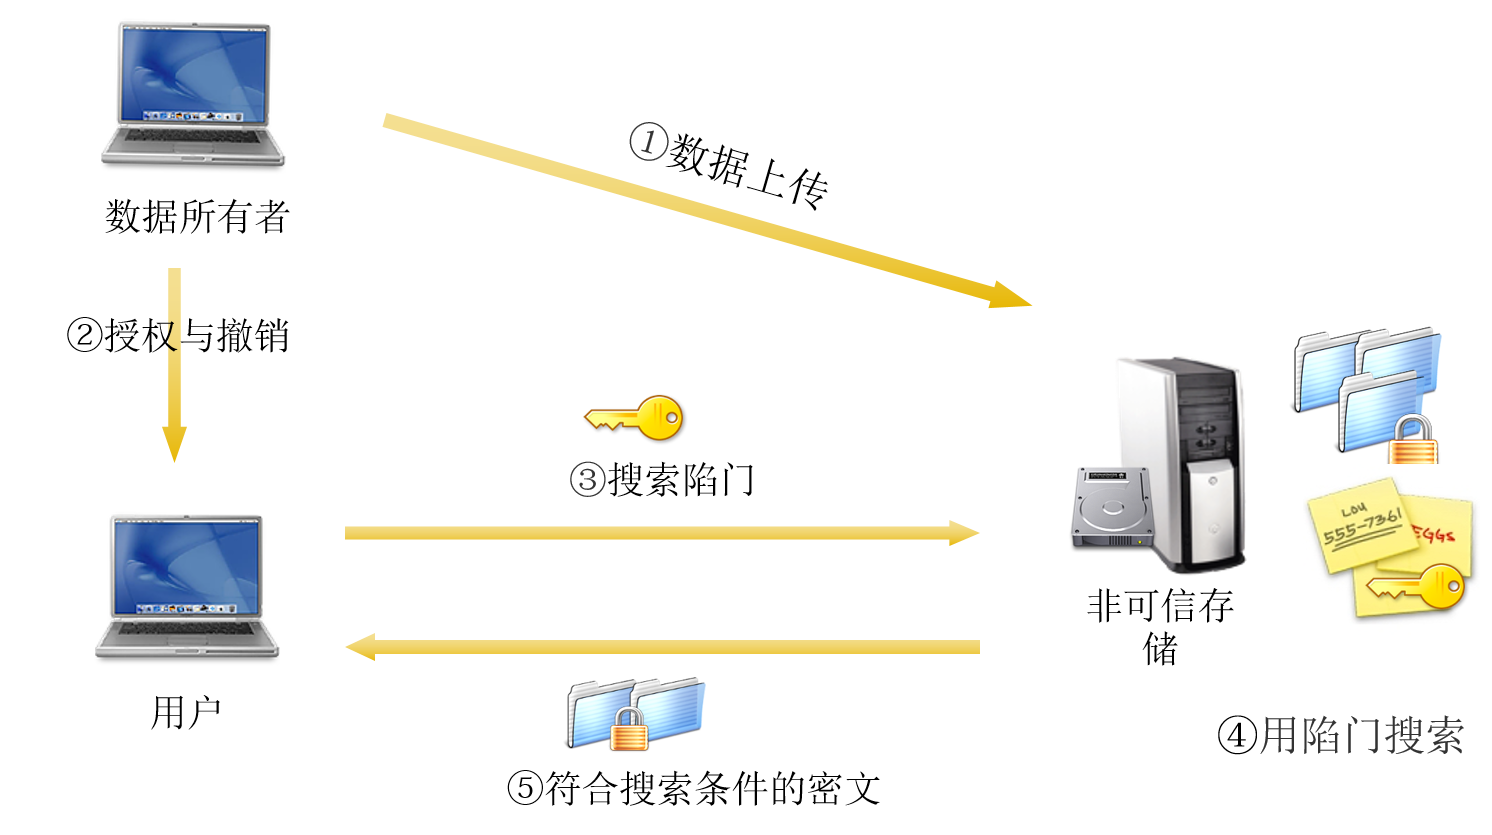
\includegraphics[width=0.9\textwidth]{chap3/general_system_model}
  \bicaption[fig:general_system_model]{对称可搜索加密的系统模型}{对称可搜索加密的系统模型}
  {Fig}{A General System Model in SSE}
\end{figure}


从图\ref{fig:general_system_model}可知,一个典型的模型有三部分组成:数据所有者、授权用户和非可信服务器。
通常数据所有者拥有数据,一个被授权的组织可以对加密的数据进行查找。过程如下:数据拥有者上传待外包的文档
并维护对加密数据的高效检索,并且对某个组织内的所有用户进行授权或撤销;被授权的用户可随时对远程加密的数据
进行搜索,并对接收的结果解密;服务器具有对加密数据进行各种条件搜索的能力,并返回符合条件的答案。我们对
数据所有者给用户进行授权和撤销的细节没有考虑,可以使用各种技术完成(公钥加密或私钥加密等) --- 仅仅传递密钥,
信息量小。



针对该系统模型,这里简单介绍一个具有代表性的基于inverted-index的对称可搜索加密方案,
该方案由五个算法组成:$SSE = (Gen, Enc, Trpdr, Search, Dec)$,数学定义如下:
\begin{enumerate}
  \item
  $Gen(1^k ) \rightarrow K$:给定安全参数$k$,生成密钥$K$;

  \item
  $Enc(K,D) \rightarrow (I,c)$:给定一组文档$D={D_1,D_2  ,…D_n  }$,使用密钥$K$加密,
  生成安全索引$I$和密文文档集合$c =\{c_1, c_2, ..., c_n \}$;


  \item
  $Trpdr(K,w) \rightarrow t_w$:给定一个单词$w$,使用密钥$K$调用陷门生成函数,输出对应的陷门$t_w$;

  \item
  $Search(I,t_w) \rightarrow R$:对陷门$t_w$在安全索引$I$上进行搜索,输出所有包含单词陷门的文档$ID$集合$R$;

  \item
  $Decrypt(K, c_i) \rightarrow D_i$:使用密钥$K$对文档$c_i$解密,生成$D_i$。

\end{enumerate}
数据拥有者首先调用$Gen$算法生成密钥并保存在本地,然后对需上传的文档调用$Enc$算法,
生成安全索引和一组加密文档,并上传至服务器。当需要检索时,用户调用$Trpdr$算法生成待搜索单词的陷门,
并发至服务器;然后服务器调用算法$Search$,使用收到的陷门在安全索引上查找,输出所有符合条件的文档$ID$,
并将对应的加密数据返回给请求者。最后,数据拥有者调用$Decrypt$算法解密加密文档。



%%%%%%%%%%%%%%%%%%%%%%%%%%%%%%%%%
%%
%%   安全模型
%%
%%%%%%%%%%%%%%%%%%%%%%%%%%%%%%%%%
\section{Non-adaptive安全模型}
\label{sec:search_symm_security_model}

%%对称可搜索加密技术(SSE)的安全证明模型与密码学中常用的安全证明模型(通常是CPA和CCA))有所不同。
%%根据实际的场景,当前SSE大多以选择关键字攻击(CKA)作为安全分析模型。这里,我们选择两个具有代表性的安全级别
%%(Non-Adaptive安全和Adaptive安全),并分别从语义安全(semantic security)和不可区分安全
%%(indistinguishability security)进行描述。这里介绍的所有知识引用自curtmola的方案\cite{curtmola2006searchable}。
%%对称可搜索加密技术(SSE)中信息泄漏主要发生在搜索阶段,以单词所携带的信息量为单位,我们以选择关键字
%%攻击(CKA)(不同于CPA和CCA)为攻击模型进行安全分析。%为此,正式的定义安全模型之前,首先定义一些基本概念。


%%对称可搜索加密技术(SSE)的安全证明模型与密码学中常用的安全证明模型(通常是CPA和CCA))有所不同。
%%根据实际的场景,当前SSE大多以选择关键字攻击(CKA)作为安全分析模型,安全级别包括Non-Adaptive安全和Adaptive安全。
%%这里,我们选择具有代表性的相对较弱的Non-Adaptive安全级别,并分别从语义安全(semantic security)和
%%不可区分安全(indistinguishability security)进行描述。这里介绍的所有知识来自curtmola的方案\cite{curtmola2006searchable}。


该小节描述的所有定义来自于curtmola的方案\cite{curtmola2006searchable}。

对称可搜索加密技术(SSE)的安全证明模型与密码学中常用的安全证明模型(通常是CPA和CCA))有所不同。
根据实际的场景,当前SSE大多以选择关键字攻击(CKA)作为安全分析模型,典型的安全级别包括Non-Adaptive安全和
Adaptive安全。在对称可搜索加密环境下的Non-adaptive和Adaptive的安全模型,如图\ref{fig:non_or_adaptive}所示:

\begin{figure}[!htp]
  \centering
  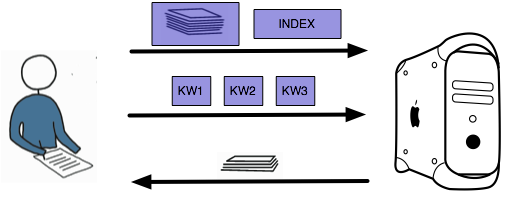
\includegraphics[width=0.45\textwidth]{chap2/non_adaptive}
  \hspace{1cm}
  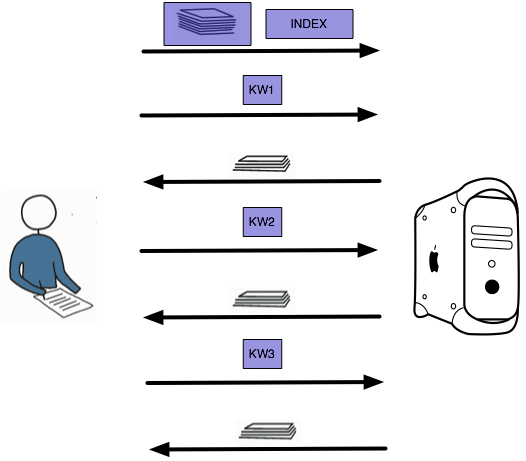
\includegraphics[width=0.45\textwidth]{chap2/adaptive}
  \bicaption[fig:non_or_adaptive]{SSE上Non-adaptive和Adaptive安全模型}{SSE上Non-adaptive和Adaptive安全模型}{Fig}{The Security Model of Non-adaptive and Adaptive in SSE}
\end{figure}

这里,我们选择具有代表性的安全等级相对较弱的Non-Adaptive模型,并分别从语义安全(semantic security)和
不可区分安全(indistinguishability security)进行描述。


%%下面我们分别给出了在对称可搜索加密环境下的Non-adaptive和Adaptive的安全模型,
%%如图\ref{fig:non_or_adaptive} 所示,然后给出相关的定义。
%%
%%\begin{figure}[!htp]
%%  \centering
%%  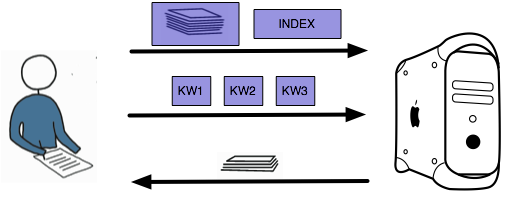
\includegraphics[width=0.45\textwidth]{chap2/non_adaptive}
%%  \hspace{1cm}
%%  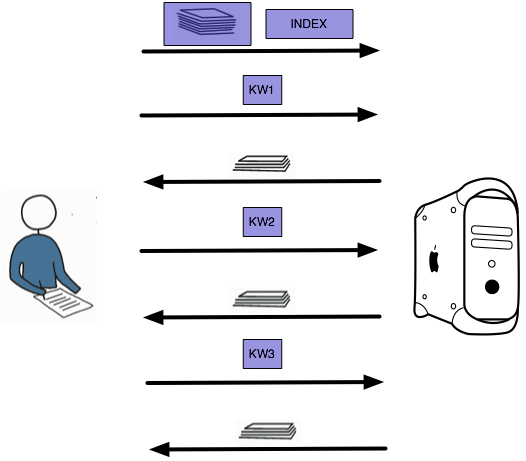
\includegraphics[width=0.45\textwidth]{chap2/adaptive}
%%  \bicaption[fig:non_or_adaptive]{SSE上Non-adaptive和Adaptive安全模型}{SSE上Non-adaptive和Adaptive安全模型}{Fig}{The Security Model of Non-adaptive and Adaptive in SSE}
%%\end{figure}


%%%%%%%%%%%%%%%%%%%%%%%%%%%%%%%%%%%%%%%%%%%%%%%%%
\begin{defn}[History]
\label{defn:attack_history}

假定$\Delta$代表单词词典,$D$表示在字典$\Delta$上的一组文档集合。
$D$上$q$次查询的历史(History) 定义为一个元组$H = (D,w)$,
其中$w$是包含$q$个单词的集合:$w = (w_1,...,w_q)$。

\end{defn}
%%%%%%%%%%%%%%%%%%%%%%%%%%%%%%%%%%%%%%%%%%%%%%%%%


%%%%%%%%%%%%%%%%%%%%%%%%%%%%%%%%%%%%%%%%%%%%%%%%%
\begin{defn}[Access Pattern]
\label{defn:attack_access_pattern}
假定$\Delta$代表单词词典,$D$表示在字典$\Delta$上的一组文档集合。
$D$上$q$次查询历史$H = (D,w)$的访问模式(Access Pattern)定义为一个元组 $ \partial (H)=(D(w_1 ),…,D(w_q))$。
\end{defn}
%%%%%%%%%%%%%%%%%%%%%%%%%%%%%%%%%%%%%%%%%%%%%%%%%



%%%%%%%%%%%%%%%%%%%%%%%%%%%%%%%%%%%%%%%%%%%%%%%%%
\begin{defn}[Search Pattern]
\label{defn:attack_search_pattern}
假定$\Delta$代表单词词典,$D$表示在字典$\Delta$上的一组文档集合。$D$上$q$次查询历史 $H=(D,w)$的搜索模式(Search Pattern)定义为对称二元矩阵$ \sigma(H) = \left(
  \begin{array}{cccc}
     x_{1,1} & x_{1,2} & ... & x_{1,q}  \\
    . & . & ... & . \\
    . & . & ... & . \\
     x_{q,1} & x_{q,1} & ... & x_{q,q}  \\
  \end{array}
\right)$ 。对于任意$1 \leq i,j \leq q$,如果$w_i = w_j$,则$x_{i,j}$为1,否则为0。
\end{defn}
%%%%%%%%%%%%%%%%%%%%%%%%%%%%%%%%%%%%%%%%%%%%%%%%%

%%%%%%%%%%%%%%%%%%%%%%%%%%%%%%%%%%%%%%%%%%%%%%%%%
\begin{defn}[Trace]
\label{defn:attack_trace}
假定$\Delta$代表单词词典,$D$表示在字典$\Delta$上的一组文档集合。$D$上$q$次查询历史 $H = (D,w)$的Trace定义为:$τ(H)=(|D_1 |,...,|D_n |,\partial(H),\sigma(H))$,其中$|D_i |(1 \leq i \leq n)$代表第$i$ 个文档的长度。
\end{defn}
%%%%%%%%%%%%%%%%%%%%%%%%%%%%%%%%%%%%%%%%%%%%%%%%%


\begin{defn}[Non-singular history]
\label{defn:attack_non_singular_history}
如果对任意的历史$H$满足:(1)至少存在一个历史 $H' \neq H$,使$\tau(H') = \tau(H)$;(2)在给定的$\tau(H)$ 下,历史$H'$可以在多项式时间内被发现;则称历史$H$是Non-singular。
\end{defn}
%%%%%%%%%%%%%%%%%%%%%%%%%%%%%%%%%%%%%%%%%%%%%%%%%






\subsection{\textbf{Non-Adaptive不可区分安全}}
\label{sec:search_symm_security_model_nonadaptive_indist_security}

%%
%% definition 2.13
%%
\begin{defn}[Non-adaptive Indistinguishability]
\label{defn:non_adaptive_indistinguishability}
在词典为$\Delta$,安全参数为$k \in \mathbb{N}$的基础上,设$SSE = (Gen, Enc, Trpdr, Search,Dec)$是一个基于安全索引的对称可搜索加密方案,
且$\mathcal{A}=(\mathcal{A}_1,\mathcal{A}_2)$为$non-uniform$的敌手,考虑下面的概率试验${\textbf{Ind}}_{(SSE,\mathcal{A})}(k)$:
\begin{center}
\begin{tabular}{ l  }
    $\textbf{Ind}_{SSE,\mathcal{A}}(k)$                           \\
    \quad $K \leftarrow Gen(1^k)$                       \\
    \quad $(st_\mathcal{A},H_0,H_1) \leftarrow \mathcal{A}_1(1^k)$          \\
    \quad $ b \overset{\$}{\leftarrow} {0,1}$           \\
    \quad parse $H_b$ as $(D_b,w_b)$                    \\
    \quad $(I_b,c_b) \leftarrow Enc_K(D_b)$             \\
    \quad $for 1 \leq i \leq q $                        \\
    \quad \quad $t_{b,i} \leftarrow Trpdr_K(w_{b,i})$   \\
    \quad let $t_b = (t_{b,1}, ..., t_{b,q})$           \\
    \quad $b' \leftarrow \mathcal{A}_2(st_\mathcal{A},I_b,c_b,t_b)$         \\
    \quad if $b' = b$, output 1                         \\
    \quad otherwise output 0
\end{tabular}
\end{center}
假设在$\tau(H_0) = \tau(H_1)$,$st_\mathcal{A}$ --- 表示敌手$\mathcal{A}$的状态信息的前提下,如果对于任意多项式的敌手$\mathcal{A}$,有:
\begin{center}
$Pr[\textbf{Ind}_{SSE,\mathcal{A}}(k) = 1] \leq \frac{1}{2} + negl(k)$,\\
\end{center}
则称该SSE方案在Non-adaptive不可区分的条件下是安全的。
\end{defn}



\subsection{\textbf{Non-Adaptive语义安全}}
\label{sec:search_symm_security_model_nonadaptive_semantic_security}
%%
%% definition 2.14
%%
\begin{defn}[Non-adaptive Semantic Security]
\label{defn:non_adaptive_semantic_security}
在词典为$\Delta$,安全参数为$k \in \mathbb{N}$基础上,设$SSE = (Gen, Enc, Trpdr, Search, Dec) $是一个基于安全索引的对称可搜索加密方案,$\mathcal{A}$为一个敌手,$\mathcal{S}$是一个模拟器(Simulator),考虑下面概率过程:
\begin{center}
\begin{tabular}{ l l }
    $\textbf{Real}_{SSE,\mathcal{A}}(k)$  &  $\textbf{Sim}_{SSE,\mathcal{A},\mathcal{S}}$    \\
    \quad $K \leftarrow Gen(1^k)$   &   \quad $(H,st_\mathcal{A}) \leftarrow \mathcal{A}(1^k)$ \\
    \quad $(st_\mathcal{A},H) \leftarrow \mathcal{A}(1^k)$ & \quad $V \leftarrow S(\tau (H))$ \\
    \quad parse $H$ as $(D,w)$          &   \quad output $V$ and $st_\mathcal{A}$             \\
    \quad $(I,c) \leftarrow Enc_K(D)$            &   \\
    \quad for $1 \leq i \leq q $                 &   \\
    \quad \quad $t_i \leftarrow Trpdr_K(w_i)$    &   \\
    \quad let $t = (t_i, ..., t_q)$              &    \\
    \quad output $V = (I,c,t)$ and $st_\mathcal{A}$    &
\end{tabular}
\end{center}
如果对于任何多项式规模敌手$\mathcal{A}$,都存在一个模拟器$\mathcal{S}$,使得对于任意多项式规模的区分器$\mathcal{D}$,有:
\begin{center}
$|Pr[\mathcal{D}(V,st_\mathcal{A})] = 1 : (V,st_\mathcal{A}) \leftarrow \textbf{Real}_{SSE,A}(k)] - Pr[\mathcal{D}(v,st_\mathcal{A})=1 : (V,st_\mathcal{A} \leftarrow \textbf{Sim}_{SSE,\mathcal{A},\mathcal{S}}(k)] | \leq negl(k)$,
\end{center}
则称该SSE在Non-adaptive的条件下是语义安全的。
\end{defn}




%%%%%%%%%%%%%%%%%%%%%%%%%%%%%%%%%%%%%%%%%
%%
%%
%%     Adaptive安全模型
%%
%%
%%%%%%%%%%%%%%%%%%%%%%%%%%%%%%%%%%%%%%%%%
%%%\subsection{\textbf{Adaptive安全模型}}
%%%\label{sec:search_symm_security_model_adaptive}
%%%
%%%%%
%%%%% definition 2.15
%%%%%
%%%\begin{defn}[Adaptive Indistinguishability]
%%%\label{defn:adaptive_indistinguishability}
%%%在词典为$\Delta$,安全参数为$k \in \mathbb{N}$的基础上,设$SSE = (Gen, Enc, Trpdr, Search,Dec)$是一个基于安全索引的对称可搜索加密方案,且$ \mathcal{A}=(\mathcal{A}_1, ...,\mathcal{A}_{q+1})$为$non-uniform$ 的敌手,考虑下面的概率试验${\textbf{Ind}}^{*}_{(SSE,\mathcal{A})}(k)$:
%%%\begin{center}
%%%\begin{tabular}{ l  }
%%%    $\textbf{Ind}^{*}_{SSE,\mathcal{A}}(k)$                           \\
%%%    \quad $K \leftarrow Gen(1^k)$                       \\
%%%    \quad $ b \overset{\$}{\leftarrow} {0,1}$           \\
%%%    \quad $(st_\mathcal{A},D_0,D_1) \leftarrow \mathcal{A}_0(1^k)$          \\
%%%    \quad $(I_b,c_b) \leftarrow Enc_K(D_b)$    \\
%%%    \quad $(st_A, w_{0,1}, w_{1,1}) \leftarrow \mathcal{A}_1(st_\mathcal{A},I_b)$ \\
%%%    \quad $t_{b,1} \leftarrow Trpdr_K(w_{b,1}) $   \\
%%%    \quad for $2 \leq i \leq q,$ \\
%%%    \quad \quad $(st_\mathcal{A},w_{0,i}, w_{1,i} \leftarrow \mathcal{A}_i(st_\mathcal{A},I_b,c_b,t_{b,1}, ..., t_{b,i-1}) $ \\
%%%    \quad \quad  $t_{b,i} \leftarrow Trpdr_K(W_{b,i}) $ \\
%%%    \quad let $t_b = (t_{b,1}, ..., t_{b,q})$           \\
%%%    \quad $b' \leftarrow \mathcal{A}_{q+1}(st_\mathcal{A},I_b,c_b,t_b)$     \\
%%%    \quad if $b' = b$, output 1                         \\
%%%    \quad otherwise output 0
%%%\end{tabular}
%%%\end{center}
%%%在$\tau (D_0,w_{0,1}, ..., w_{0,q}) = \tau(D_1,w_{1,1}, ..., w_{1,q})$的前提下。如果对于所有多项式规模的敌手$\mathcal{A} =(\mathcal{A}_0, ..., \mathcal{A}_{q+1})$,均有有:
%%%\begin{center}
%%%$Pr[\textbf{Ind}^{*}_{SSE,\mathcal{A}}(k) = 1] \leq \frac{1}{2} + negl(k)$,\\
%%%\end{center}
%%%则称该SSE方案在adaptive不可区分的条件下是安全的。
%%%\end{defn}
%%%
%%%%%
%%%%% definition 2.16
%%%%%
%%%\begin{defn}[Adaptive Semantic Security]
%%%\label{defn:adaptive_semantic_security}
%%%在词典为$\Delta$,安全参数为$k \in \mathbb{N}$基础上,设$SSE = (Gen, Enc, Trpdr, Search, Dec)$是一个基于安全索引的对称可搜索加密方案,$\mathcal{A} = (\mathcal{A}_0, ..., \mathcal{A}_q)$为敌手,$\mathcal{S} = (\mathcal{S}, ..., \mathcal{S}_q)$是模拟器(Simulator),考虑下面概率过程:
%%%\begin{center}
%%%\begin{tabular}{ l l }
%%%    $\textbf{Real}^{*}_{SSE,\mathcal{A}}(k)$  &  $\textbf{Sim}^{*}_{SSE,\mathcal{A},\mathcal{S}}$    \\
%%%    \quad $K \leftarrow Gen(1^k)$   &   \quad $(D,st_\mathcal{A}) \leftarrow \mathcal{A}_0(1^k)$ \\
%%%    \quad $(D,st_\mathcal{A}) \leftarrow \mathcal{A}_0(1^k)$ & \quad $(I,c,st_\mathcal{S}) \leftarrow \mathcal{S}_0(\tau(D))$ \\
%%%    \quad $(I,c) \leftarrow Enc_K(D)$  &  \quad $(w_1,st_\mathcal{A} \leftarrow \mathcal{A}_1(st_\mathcal{A},I,c)$ \\
%%%    \quad $(w_1, st_\mathcal{A}) \leftarrow \mathcal{A}_1(st_\mathcal{A},I,c)$ & \quad $(t_1,st_\mathcal{S}) \leftarrow \mathcal{S}_1(st_\mathcal{S}, \tau(D,w_1))$ \\
%%%    \quad $t_1 \leftarrow Trpdr_K(w_1)$   & \quad for $ 2 \leq i \leq q$  \\
%%%    \quad for $2 \leq i \leq q $         &  \quad \quad $(w_i,st_\mathcal{A}) \leftarrow \mathcal{A}_i(st_\mathcal{A},I,c,t_1, ..., t_{i-1})$      \\
%%%    \quad \quad $(w_i,st_\mathcal{A}) \leftarrow \mathcal{A}_i(st_\mathcal{A},I,c,t_1, ..., t_{i-1})$    &   \quad \quad $(t_i,st_\mathcal{S}) \leftarrow \mathcal(S)_i(st_\mathcal{S}, \tau(D,w_1, ..., w_i))$  \\
%%%    \quad \quad $t_i \leftarrow Trpdr_K(w_i)$    & \quad let $t = (t_1, ..., t_q)$  \\
%%%    \quad let $t = (t_1, ..., t_q)$              &   \quad output $V = (I,c,t)$ and $st_\mathcal{A}$ \\
%%%    \quad output $V = (I,c,t)$ and $st_\mathcal{A}$    &
%%%\end{tabular}
%%%\end{center}
%%%如果对于任何多项式规模敌手$\mathcal{A} = (\mathcal{A}_0, ..., \mathcal{A}_q)$,都存在模拟器$\mathcal{S} = (\mathcal{S}, ..., \mathcal{S}_q)$,使得对于任意多项式规模的区分器$\mathcal{D}$,有:
%%%\begin{center}
%%%$|Pr[\mathcal{D}(V,st_\mathcal{A})] = 1 : (V,st_\mathcal{A}) \leftarrow \textbf{Real}^*_{SSE,A}(k)] - Pr[\mathcal{D}(v,st_\mathcal{A})=1 : (V,st_\mathcal{A}) \leftarrow \textbf{Sim}^*_{SSE,\mathcal{A},\mathcal{S}}(k)] | \leq negl(k)$,
%%%\end{center}
%%%则称该SSE在adaptive的条件下是语义安全的。
%%%\end{defn}
%%%
%%%Curtmola在论文\cite{curtmola2006searchable}中分别证明Non-adaptive不可区分安全性与Non-adaptive语义安全和adaptive不可区分安全性与adaptive语义安全是等价的。
%%%

%%%%%%%%%%%%%%%%%%%%%%%%%%%%%%%%%%%%%%%%%%%%%%%%%%%%%
%%
%%      对称可搜索加密技术
%%
%%%%%%%%%%%%%%%%%%%%%%%%%%%%%%%%%%%%%%%%%%%%%%%%%%%%%
\section{对称可搜索加密方案分类}
\label{sec:search_symm_symm}


%%%%%%%%%%%%%%%%%%%%%%%%%%%%%%%%%%
%%
%%  单关键字搜索
%%
%%%%%%%%%%%%%%%%%%%%%%%%%%%%%%%%%%
\subsection{单关键字搜索}
\label{sec:search_symm_symm_exact}

对于可搜索加密问题,Goh在文章\cite{goh2003secure}中的提出了第一个基于正向索引的解决方案。
方案使用一个Bloom Filter\cite{gremillion1982designing}作为安全索引。
对于每个文档,映射包含的所有单词到一个Bloom Filter;在搜索时,授权用户发送待查单词的多个哈希
值作为陷门;一旦服务器收到请求后,逐个检查每个Bloom Filter,判断对用的位置是否是“1”,
如果全部都为“1”,则表示包含该单词并返回该文档,否则跳过。该方案突出的优势体现在性能上:
Bloom Filter的映射过程只需要计算若干Hash函数,故索引创建过程性能较高。在搜索阶段,
服务器需要对每个文档调用一次SearchIndex算法,而在该算法中对陷门中每个元素只需进行Bloom
Filter数据位的比较操作,时间复杂度仅为$O(1)$,故整体效率仍然是比较高的。但是该方案却引进了误报率,
且误报率和安全索引的大小成反比关系。

Y. Chang在\cite{chang2005privacy}中则基于forward-index提出了没有误报率的的方案。其基本思想如下:
将待上传文档中所有出现的单词构成一个词典,安全索引中用一比特位代表每个单词是否存在
--- “1”表示存在该单词,“0”表示不存在。方案同样达到了相当高的效率,但问题在于词典的保存大大增加
了存储开销的负担。文中给出了两个解决方案,第一个方案是将词典保存在客户端,这样用户每次查询则
需要本地词典,这样增加了本地的存储和计算开销,并且在多用户环境下还需要同步词典;第二个方案则
将词典加密后存放在远程服务器上,但查询过程则需要通讯两轮 --- 一轮获得词典里索引信息,另一轮查询
获得文档。

R.Curtmola在文章\cite{curtmola2006searchable}中第一次基于inverted-index给出了两个改进方案,
并给出了详细的安全性定义和证明。第一个方案达到了Non-adaptive安全性,其基本思想描述如下:
首先构建待上传文档的inverted-index;然后将索引表项中的文档ID部分加密并随机分散到一个数组中,
如下图\ref{fig:curtmolaInvertedIndex}所示:

\begin{figure}[!htp]
  \centering
  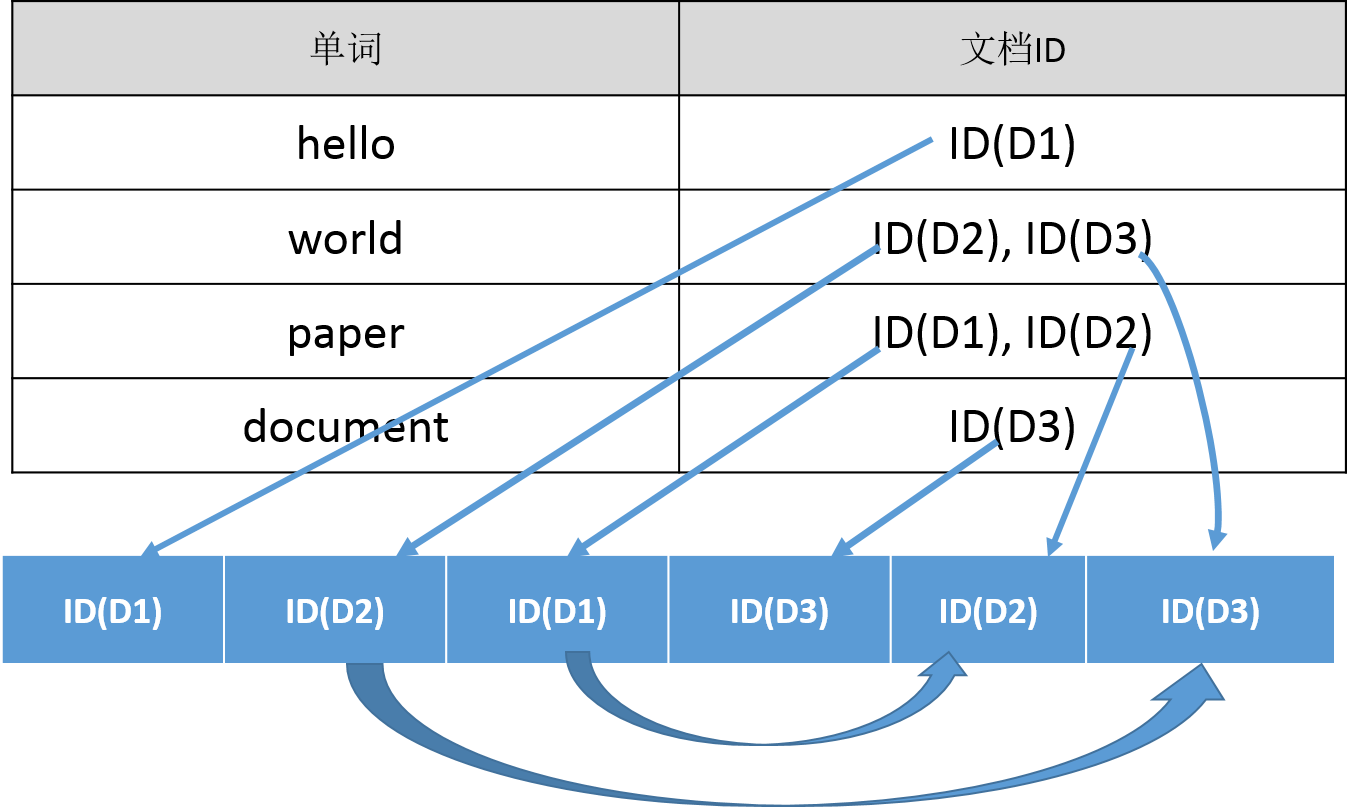
\includegraphics[width=0.8\textwidth]{chap2/curtmolaInvertedIndex}
  \bicaption[fig:curtmolaInvertedIndex]{文档ID数组}{文档ID数组}{Fig}{The Array of Document ID}
\end{figure}

从上表可知,每个单词所对应文档的ID形成一个链表。数组中的每个元素使用不同的密钥调用对称分组密码算法加密。而文档中所有的单词在Inverted-index则以查找表的形式存储,如图\ref{fig:curtmolaSearchTable} 所示:
\begin{figure}[!htp]
  \centering
  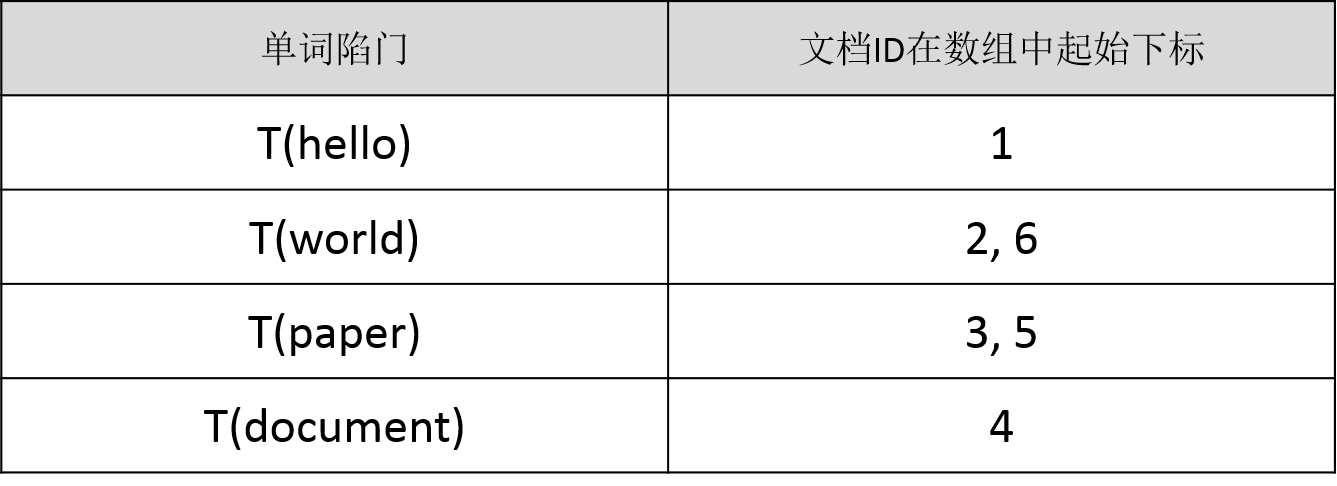
\includegraphics[width=0.8\textwidth]{chap2/curtmolaSearchTable}
  \bicaption[fig:curtmolaSearchTable]{反向安全索引中的查找表}{反向安全索引中的查找表}{Fig}{The Look-up Table of Secure Index}
\end{figure}


查找表的条目由键值对的形式表示,其键存储的是通过伪随机函数对单词置换后的结果 --- 单词的陷门,
其值所存储的部分为对应文档$ID$的链表在数组中的起始位置。
查找的时候,通过单词的陷门在查找表处找到其$ID$链表在数组中的起始位置,
然后根据起始$ID$位置逐个解密这个链表获得所有包含该单词的文档$ID$集。

Curtmola方案一的主要优势是服务器端的搜索效率高,得益于inverted-index,其服务器端搜索时间复杂度为$O(1)$,
而之前的方案都只能达到$O(n)$($n$表示文档的数目)。同时R. Curtmola在文中给出了另一个具有
Adaptive安全性的方案,服务器端搜索时间复杂度仍能保持$O(1)$,但是服务器端的存储量和单词陷门的大小均有所增加。

为了确保方案足够安全 --- 不能因$ID$链表元素个数不同而导致信息泄漏,Curtmola建议数组元素的个数应与
所有文档的总长度所能容纳的最大单词数相当。这将导致在安全索引中,数组部分所占用的存储空间将会远大于
所有文档的总长度。H. Lu在文章\cite{jin2012reducing}中基于inverted-index提出了一种降低安全索引
结构所占存储空间的方案。方案与Curtmola在方案1的最大不同在于合并了安全索引中$ID$链表结构中相同的
元素,从而极大减少了数组的长度,如图\ref{fig:luInvertedIndex}所示:
\begin{figure}[!htp]
  \centering
  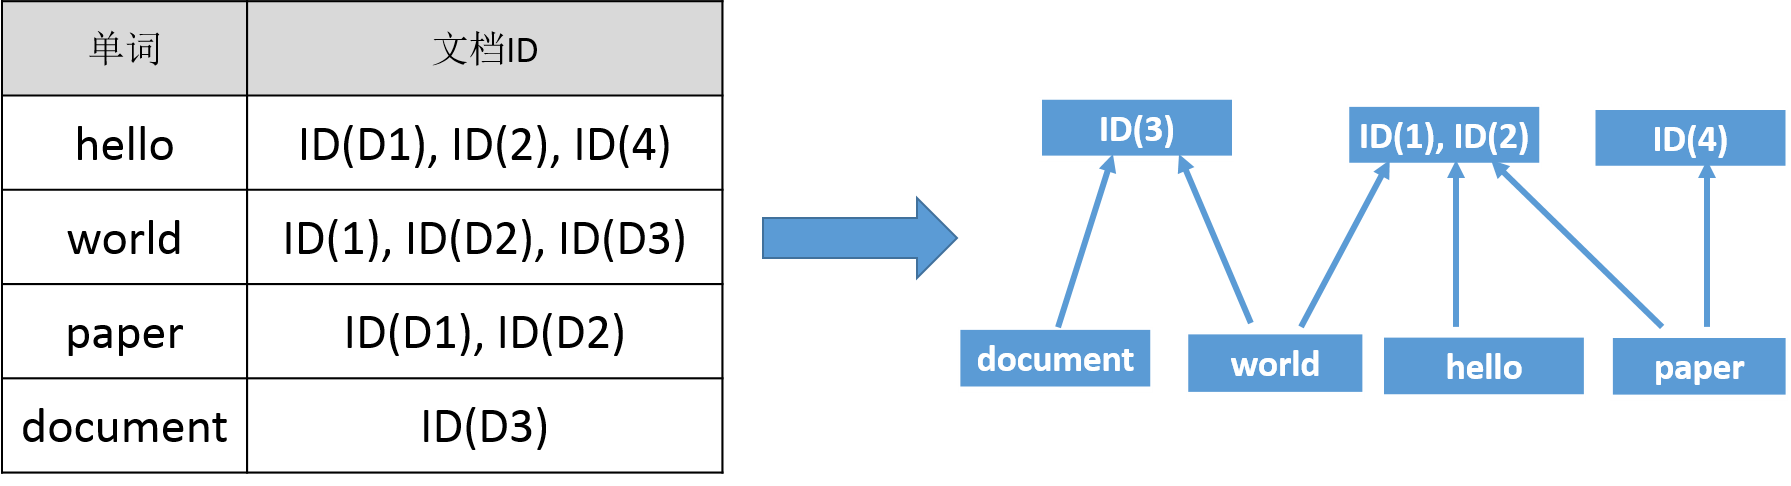
\includegraphics[width=0.8\textwidth]{chap2/luInvertedIndex}
  \bicaption[fig:luInvertedIndex]{改进的文档ID链表}{改进的文档ID链表}{Fig}{An Improved List of Documents ID}
\end{figure}

基于这样的结构使得合并后每个文档$ID$在数组中只出现一次,从而减少数组元素的总数。经实际测试,
方案中数组的元素个数可降至原来的5\%以下。

作者Van在\cite{van2010computationally}中基于inverted-index提出了另一种形式的安全索引方案,
方案使用一个加密的二元数组维护安全索引信息,数组两维分别表示单词和文档$ID$,数组元素为“1”表示对应
的文档包含对应的单词。搜索时解密二维数组中对应单词所在的行,即可知晓包含该单词的文档$ID$。



\subsection{模糊搜索}
\label{sec:search_symm_symm_fuzzy}

在加密的云数据环境中,当前的相似搜索的研究集中在模糊搜索上。基于明文模糊搜索\cite{ji2009efficient}
\cite{li2008efficient} \cite{behm2009space} 和精确关键字搜索\cite{curtmola2006searchable}
\cite{chang2005privacy} \cite{jin2012reducing},Jin Li等人于2010年在\cite{li2010fuzzy}中率先提出了
模糊对称可搜索加密的问题,并提供了两种解决方案:直接模糊搜索方案和基于通配符的模糊搜索方案。方案用
编辑距离(edit distance\cite{ristad1998learning})来衡量单词之间的相似性,即若给定单词$w_1$和$w_2$,
定义其编辑距离为:将$w_1$变换成$w_2$所需的最小的操作数,变换操作包括:(1)插入:在单词的某个位置上
插入一个字符;(2)删除:删除单词中某个字符;(3)替换:将单词中某个字符替换为另一个字符。该方案的基
本思想如下:(1)加密阶段:对文档集中每个单词$w$构建模糊集$F_w$,用与\cite{curtmola2006searchable}方
案相同方式构建反向安全索引,然后将安全索引和加密文档外包;(2)陷门生成阶段:当搜索单词$w$时,首先构
建单词$w$的模糊集$F_w$,然后计算集合$F_w$所有单词的陷门并提交至服务器;(3)搜索阶段:当服务器收到请
求的陷门后,在安全索引中查询是否存在和单词$w$的陷门精确匹配的索引,若存在则返回,否则返回与模糊集
$F_w$所有陷门匹配的结果。

在直接的模糊搜索方案中,构建单词$w$的模糊集如下:枚举所有的单词$w'$使得$ed(w,w') \leq d$。
而在改进的模糊搜索方案中,用通配符来替代同一位置上所有不同的单词,这样大大降低了模糊集的规模,
降低了网络传输开销和服务端的存储开销。但是不幸的是,方案对服务器存储开销与编辑距离正相关,
且不支持多关键字搜索。同时,不同单词的模糊集之间存在碰撞,例如当单词$“at”$ 和$“it”$ 在编辑距离为1时,
对应模糊集分别为:$S_{at,1}=\{*at,*t,a*t,a*,at*\}$, $S_{it,1}= \{*it,*t,i*t,i*,it* \}$($S_{w,d}$
表示单词$w$在编辑距离为$d$时的模糊集),有$S_{at,1} \cap  S_{it,1} \neq \varnothing $。

为了解决上述方案中服务端存储过大的问题,M. Chuah等人在\cite{chuah2011privacy}中提出了基于
BedTree\cite{zhang2010bed}的模糊可搜索加密方案。方案的具体过程如下:(1)加密阶段:对于单
词$w$在编辑距离为$d$时,将其模糊集对应的陷门映射到Bloom Filter中,
如将$S_{w,i}$ 映射到$B_i$中($S_{w,i}$ 表示单词$w$在编辑距离为$i$时的模糊集,
$B_i$表示编辑距离为$i$时模糊集所构造的Bloom Filter),然后将单词的$ \{B_i, i \leq d \}$、
单词所对应文档的ID信息以及单词的陷门作为一个叶子节点,通过单词的数据向量插入到BedTree树中;
(2)陷门生成阶段:对待搜索单词$w$,计算其数据向量和模糊集中每个元素的陷门,并提交至服务端;
(3)搜索阶段:当服务器收到用户的查询信息后,首先通过其数据向量在BedTree树构造的安全索引中
查找某叶子节点,再检查模糊集陷门是否存在于$B_i$中,最终返回正确匹配的结果集。该方案主要在安全
索引结构上有所改进,利用BedTree的索引结构降低了存储空间和Bloom Filter减少了索引构建时间,
同时能很好地扩展到多关键词搜索和增量更新。然而,方案也引入了新的的问题 --- 由Bloom Filter引入
了一定的误报率。

Cong Wang等人在\cite{wang2012achieving}中基于Trie树的结构提出了搜索效率更高且具备同等安全的模糊可
搜索加密方案。他们首先对方案\cite{li2010fuzzy}提出了改进措施:对每个单词$w$,根据容许的最大编辑距离
$d$计算出单词的模糊集$S_{w,d}$,然后根据Bloom Filter技术将每个单词的模糊集计算出的令牌映射到一个
Bloom Filter,即对每个关键字的模糊集构建一个Bloom Filter;在搜索关键字$w$时,
服务端只需搜索待搜索单词模糊集对应令牌是否存在某个Bloom Filter中,即可查询得到所需的结果。
基于\cite{li2010fuzzy}的改进方案虽然减少服务器的存储量,但是却增加了服务端的搜索时间 ---
对所有关键字构建的Bloom Filter索引都要搜索一次,并且由Bloom Filter结构带来了一定的误报率。
方案的构建过程如下:(1)加密阶段:首先计算文档中每个单词的模糊集和对应令牌信息。然后对于每个令牌将其分成N块,并将N块的子结构插入到Trie 树中,叶子节点即单词令牌的最后一块,并将单词对应文档信息放在叶子节点中或者在当前叶子节点下插入一个新的节点存放其他信息,最后将安全索引和文档密文外包到服务端;(2)陷门生成阶段:对单词$w$,计算模糊集及对应令牌,并发送给服务端;(3)搜索阶段:当服务端收到用户发来的令牌集后,首先对单词$w$的令牌按照构建索引过程分成N块,然后在基于Trie树的索引中进行精确查找,若找到返回精确查询的结果,否则对其模糊集令牌按照同样方式搜索并返回结果集。该方案主要基于不同单词之间存在相同的部分,通过相同的部分来减少存储量。该方案与方案\cite{li2010fuzzy}相比,明显减少了服务端的存储开销但是增加了常量的搜索时间。与方案\cite{chuah2011privacy}相比,该方案减少了搜索过程中信息的泄漏增强了方案的安全性,但是从数据的时间局部性和空间局部性的角度来看,由于BedTree是一颗B+树,而Trie是一棵多叉树,因而B+树可以利用数据局部性原理来通过减少内存在访问过程中搜索失效时数据内存时间换入换出来提高单词的搜索时间。

Deshpande等人在\cite{balamuralikrishna2013fuzzy}中对目前所有模糊可搜索加密方案进行了总结 --- 包括
一般的基于通配符构建模糊集的可搜索加密方案、基于BedTree树构建索引的模糊可搜索加密方案和基于Trie树
构建索引的模糊可搜索加密方案;并提出了两种高效的模糊单词集构建方案 --- 基于通配符和Gram;并通过实
验分析了各方案在不同编辑距离时索引构建的时间和搜索的时间及个方案相关优缺点。

上述方案都以编辑距离来衡量单词间的模糊程度,不可避免带来了碰撞,引入了安全隐患。为此,
\cite{boldyreva2014efficient}第一次提出了sub-linear的模糊可搜索加密方案。在方案中,
他们使用了基于有权图的理论来描述单词间的相似性,并对此提出了一个更强的安全定义,
证明之前方案并不能达到此安全。此外,他们也给出了如何在安全性和高效性做出平衡。

\subsection{动态搜索}
\label{sec:search_symm_symm_dynamic}

基于正向索引的解决方案\cite{goh2003secure} \cite{chang2005privacy}等都能很好地适应与动态的搜索领域。
对于扩展于动态搜索,索引结构的调整非常简单,仅需要在正向索引中添加或删除对应条目即可。但是正向索引
的方案在查找上效率并不高,通常与文档数目相关。

为了解决上述方案中的不使用问题,Kamara等人于2012年在\cite{kamara2012dynamic}中第一次提出了
动态可搜索加密技术的问题及相应的解决方案。在文中作者主要结合了正向索引具有的动态修改特性和
反向索引的强安全性和无误报率等特征,在反向索引方案的基础上通过增加另一个正向索引,实现了具有
动态修改的可搜索加密方案。该方案不仅获得了有效的搜索时间 --- 线性搜索时间(与文档数目成正比),
而且确保了搜索过程中的信息泄漏,具有Non-adaptive的安全性。该方案的主要思想如下:在索引构建阶段,
不但对每个单词构建了一个反向索引,而且对每篇文档构建了一个正向索引,正向索引和反向索引通过对偶
节点(dual node)联系起来(所谓对偶节点即将正向索引结构中的<文档,单词>条目和反向索引结构中的<单词,文档>条目具有相同值的那对节点称为对偶节点);在搜索时,只需要查询反向安全索引即可;而在添加或删除文档时,需通过一系列复杂的位操作对正向索引和方向索引进行更新,同时维护正向索引与反向索引之间的对应关系。随后,Kamara在文章\cite{kamara2013parallel}中对\cite{kamara2012dynamic}方案进行扩展,提出具有并行特征的动态可搜索加密方案,这样可充分利用基于多核和分布式的计算机来提升方案的整体性能。但是服务器端额外存储量增加了1倍以上。

Stefanov等人在\cite{stefanov2013practical}中提出了具有更少信息泄漏和更高效的动态可搜索加密方案。
他们指出Kamara方案中泄漏的信息并不仅仅限于他们方案中所定义的信息 ---
泄漏搜索模式(search pattern)\cite{liu2014search}、
访问模式(access pattern)\cite{islam2012access}和大小模式(size pattern),
同时也存在forward privacy(即在搜索单词$w$后,然后立即添加一个包含$w$的文档,
服务器不应该了解到新添加的文档包含用户刚搜索过的单词$w$)和backward privacy
(即当删除包含某单词$w$的文档后,随之搜索单词$w$,服务器不应该了解到刚被删除的文档包含单词$w$)
的信息泄漏。作者在文中第一次提出具有forward privacy安全的动态可搜索加密方案,
但是backward privacy的信息泄露问题仍然没有得到解决。


\subsection{优先级搜索}
\label{sec:search__symm_symm_ranked}
支持优先级搜索的可搜索加密技术(Ranked Keyword Search)是指对于文档中出现的单词,其对应的搜索结果
文档具有不同的优先级 --- 如文档中被搜索单词出现次数多则优先级高,反之则优先级低。搜索时,
服务器按优先级先后次序返回搜索结果,或者返回指定数量的优先级最高的文档。最简单的做法将客户端预先
计算的优先级加密存放到安全索引中,搜索的时候,服务器解密搜索结果文档所对应的优先级,从而进行筛选
或排序。但A. Swaminathan在\cite{swaminathan2007confidentiality}中证实:如果服务器能直接获得优先
级值的话,在特定情况下,有可能获得明文或者搜索关键词的信息。

上述方案仅仅能将结果返回给用户,不能对结果进行过滤,例如搜索结果按优先级排序。C. Wang
在\cite{wang2010secure}\cite{wang2012enabling}中最先考虑了支持单个单词的优先级对称可搜索加密技术,
给出了这类方案的具体定义,并设计了一个具体的方案。方案中对文档的优先级使用保序加密
(Order Preserving Encryption)\cite{boldyreva2011order}技术进行加密;
对于不同的单词,使用不同的密钥加密优先级。使得服务器无法得到优先级的具体值,甚至无法评估不同关键词对
应搜索结果的优先级差异,从而降低了信息泄漏,使其安全性能与之前的对称可搜索加密方案相当。

N. Cao在\cite{cao2014privacy}中将优先级搜索问题扩展到多个单词的情形,
通过coordinate matching\cite{witten1999managing}综合考虑一篇文档相对于多个搜索单词的综合优先级,
并给出了具体的支持多个搜索单词的优先级搜索方案。该方案的问题在于单词词典是固定的,如果需要增加新
的单词的话,需要进行重构操作。Z. Xu在\cite{xu2012efficient}中针对这个问题作出了改进,使得新增单
词时,只需要少量调整操作;方案中还考虑了单词访问频率对优先级的影响。J. Yu则在\cite{cao2014privacy}中
做了进一步的研究,给出了安全性更强的方案。

%%%
%%%\subsection{优先级搜索}
%%%\label{sec:search__symm_symm_ranked}
%%%支持优先级搜索的可搜索加密技术(Ranked Keyword Search)是指对于文档中出现的单词,其对应的搜索结果文档具有不同的优先级——如文档中被搜索单词出现次数多则优先级高,反之则优先级低。搜索时,服务器按优先级先后次序返回搜索结果,或者返回指定数量的优先级最高的文档。最简单的做法将客户端预先计算的优先级加密存放到安全索引中,搜索的时候,服务器解密搜索结果文档所对应的优先级,从而进行筛选或排序。但A. Swaminathan在[42]中证实:如果服务器能直接获得优先级值的话,在特定情况下,有可能获得明文或者搜索关键词的信息。
%%%C. Wang在[40][41]中最先考虑了支持单个单词的优先级对称可搜索加密技术,给出了这类方案的具体定义,并设计了一个具体的方案。方案中对文档的优先级使用保序加密(Order Preserving Encryption)[45]技术进行加密;对于不同的单词,使用不同的密钥加密优先级。使得服务器无法得到优先级的具体值,甚至无法评估不同关键词对应搜索结果的优先级差异,从而降低了信息泄漏,使其安全性能与之前的对称可搜索加密方案相当。
%%%N. Cao在[46]中将优先级搜索问题扩展到多个单词的情形,通过coordinate matching[47]综合考虑一篇文档相对于多个搜索单词的综合优先级,并给出了具体的支持多个搜索单词的优先级搜索方案。该方案的问题在于单词词典是固定的,如果需要增加新的单词的话,需要进行重构操作。Z. Xu 在[48]中针对这个问题作出了改进,使得新增单词时,只需要少量调整操作;方案中还考虑了单词访问频率对优先级的影响。J. Yu则在[49]中做了进一步的研究,给出了安全性更强的方案。
%%%
%%%
%%%
%%%\subsection{布尔搜索}
%%%\label{sec:search_symm_symm_boolean}
%%%文档搜索中的布尔搜索(boolean search)是指搜索条件为多个单词通过逻辑与或非操作连接的表达式的情形。
%%%支持布尔搜索最简单的做法对搜索条件中的每个单词应用一次单个单词的搜索算法,然后构造一个横坐标为搜索条件中的单词,纵坐标为文档ID的二元矩阵:矩阵元素为1表示对应文档中包含对应的单词,反之为0。将搜索条件表达式中的单词替代为矩阵中对应的行,最后通过按位计算的方式计算该表达式,计算结果中的“1”所对应的文档就是搜索结果。如搜索条件为(computer∨encryption)∧¯commercial时,假定通过三次单个单词的搜索,得出包含computer的文档ID为(1, 2, 4),包含encryption的文档ID为(2, 4),包含commercial的文档ID 为(4, 5),构造图7 二元矩阵如图7 所示:
%%%
%%%	单词-文档ID二元矩阵范例
%%%将对应的行代入到搜索条件中并计算:(11010∨01010)∧¯00011=11000,可知文档1和2 为搜索结果。
%%%但上述做法泄漏了过多的信息——搜索表达式中每个单词单独的搜索结果。一个安全的支持布尔搜索的可搜索加密方案应使服务器只知晓搜索表达式的搜索结果,但无法从这个过程推导表达式中每个单词单独的搜索结果或其他搜索表达式的搜索结果。
%%%
%%%P. Golle在[17]中提出了最早的支持逻辑与的布尔搜索(conjunctive search)的对称可搜索加密方案。该方案为每个文档创建一个安全索引,索引中包含文档单词及其位置信息,搜索时需提供所有参与逻辑与操作的单词陷门及其对应的位置,只有单词和位置都符合的文档才会作为搜索结果。如某文档的前五个单词分别是(alice sent this email yesterday),当搜索(1, 5, alice, yesterday)(即第一个单词为alice,第五个单词为yesterday)时,该文档将成为搜索结果的一部分;当搜索(2, 5, alice, yesterday)时,则不作为搜索结果,因为位置不对。
%%%P. Golle在文中提出了两个可证明安全的方案。第一个方案基于Decision Diffie-Hellman困难问题[18]。 构建安全索引时需要对每个单词进行一次模指数运算,搜索过程中需要对每个文档进行两次模指数运算,而且陷门的长度与文档总数成正比关系。第二个方案基于双线性映射(bilinear map),可实现常数级别的陷门长度,创建安全索引的计算量也与第一个方案大致相当,但搜索过程对每个文档所需进行的双线性映射计算次数与搜索条件中所包含的单词数成正比。
%%%上述两个方案性能均较低,只适合从文档中提取少量关键词创建安全索引,支持在这些关键词上的搜索。一个可能的应用场景是支持对电子邮件关键域信息的搜索。
%%%L. Ballard在[19]中给出了两个支持逻辑与布尔搜索的改进方案。第一个方案基于Shamir的门限秘密分享方案[20],另一个方案则是基于双线性映射。这两个方案的效率比起[17]均大为提高,第二个方案虽然也基于双线性映射,但仅有服务器端需要进行双线性映射运算。上述两个方案同样在安全索引中包含文档单词及其位置信息,只有单词和位置都符合的文档才会作为搜索结果。
%%%K. Florian在[21]中给出了一种不保存单词位置的支持逻辑与布尔搜索的方案。在这种方案中,只要文档中包含搜索条件中的所有单词,就会加入到搜索结果,而不管这些单词出现在什么位置。在该方案中,创建安全索引时需要对每个单词进行模指数运算,创建陷门和搜索时需要进行双线性映射计算,其次数与搜索条件中的单词数成正比,故整体性能较低。D. Cash在[79]中给出了一种基于Oblivious Cross-Tags的布尔搜索算法,平衡性能和安全性。
%%%以上方案均在搜索时仅能支持单词的逻辑与操作。到目前为止,唯一能同时全面支持逻辑与或非布尔搜索的方案由T. Moataz在[22]中提出的。该方案先将所有文档中出现的单词转换成相互独立的矢量,然后通过Gram-Schmidt过程[23]将其转换成一组正交基,也就是每个单词映射到一个正交基上。对于每个文档,将其包含的单词所对应正交基的和——在这个线性子空间中每个维度的坐标都是1 的矢量——作为文档的安全索引。对于只包含逻辑与的搜索表达式,在表达式中所包含的单词对应的正交基张成的线性子空间中,精心选择一个各个维度值都不为0的矢量作为陷门,搜索时只需将陷门与安全索引进行内积运算,将结果为1的文档加入搜索结果中即可。T. Moataz还进一步讨论了支持逻辑或和逻辑非的做法。该方案可以达到Adaptive语义安全。
%%%上述方案在支持布尔搜索方面,功能相当全面,但仍然存在性能和客户端存储量的问题。在作者的测试中,当单词总数达到4000个时,创建正交基需要18秒,创建时间与单词总数的平方成正比。由于该正交基在生成搜索条件陷门的时候需要使用,从计算时间来看不适合临时生成,而应该一次生成永久保存在客户端,这就增加了客户端的存储量需求。另外,无论是否保存正交基,都需要在客户端保存一个单词词典。该方案的另一个问题是动态性,当需要进行文档增加和修改操作时,如果增加了新的单词,则需要进行正交基重构,之前所有文档的安全索引都将无效;用户必须自行下载所有文档,解密并重新创建安全索引,完成后重新上传。
%%%






%%%%
%%%%%%%%%%%%%%%%%%%%%%%%%%%%%%%%%%%%%%%%%%%%%%%%%%%%%%%%%
%%%%%%
%%%%%%      公钥可搜索加密技术
%%%%%%
%%%%%%%%%%%%%%%%%%%%%%%%%%%%%%%%%%%%%%%%%%%%%%%%%%%%%%%%%
%%%%\section{公钥可搜索加密技术}
%%%%\label{sec:asym}
%%%%
%%%%
%%%%\subsection{公钥可搜索加密的基本定义}
%%%%\label{sec:asym_defintion}
%%%%
%%%%D. Boneh在[52]中最早定义了公钥可搜索加密方案的模型:
%%%%一个非交互公钥可搜索加密方案包含以下多项式时间随机算法:
%%%%\begin{enumerate}
%%%%  \item
%%%%  {$ KenGen(s) $}:根据输入的安全参数s,生成公私钥对 $A_pub$,$A_priv$;
%%%%
%%%%
%%%%  \item
%%%%  {$ PEKS(A_pub,W) $}:以单词W和公钥 $A_pub$ 作为输入,生成单词W的可搜索密文S;
%%%%
%%%%
%%%%  \item
%%%%  {$ Trapdoor(A_priv,W) $}:根据私钥 $A_priv$ 和单词W,生成搜索陷门 $T_w$;
%%%%
%%%%
%%%%  \item
%%%%  {$ Test(A_pub,S,T_w) $}:根据密文S、陷门 $T_w$ 以及公钥 $A_pub$,测试陷门对应的单词与密文所加密的单词是否相当,如相等则输入“yes”,否则输出“no”。
%%%%
%%%%\end{enumerate}
%%%%	
%%%%	
%%%%数据接收者调用$KenGen$算法生成自己的公私钥对,并发布公钥。数据拥有者以接收者的公钥使用传统方法加密文档,并将文档中允许搜索的单词与接收者的公钥作为输入调用PEKS算法进行加密,然后将所有PEKS密文与加密文档一起发送至非可信服务器。数据接收者要进行搜索时,以自己的私钥和待搜索的单词作为输入调用Trapdoor算法,生成待搜索单词的陷门,并发往服务器。服务器对于发往接收者的每个文档,将陷门与文档的每个PEKS密文调用一次Test算法,如果存在某次Test结果为yes,则将该文档加入到搜索结果中。
%%%%从模型中可以看出,公钥可搜索加密方案是对单词进行加密,而不是像对称可搜索加密方案那样对文档或者文档集合进行加密。在这种模型下,无法使用索引技术进行加速,而且公钥运算本身效率较低,故公钥可搜索加密往往只支持对文档中的少量单词进行搜索,而不支持全文搜索。
%%%%
%%%%D. Boneh在[52]中也定义了公钥可搜索加密方案的安全性:
%%%%公钥可搜素加密方案应保证PEKS算法生成的密文不泄漏明文或者密钥的任何信息,除非敌手得到了对应的陷门。定义PEKS安全游戏如下:
%%%%\begin{itemize}
%%%%  \item
%%%%  挑战者运行 $KeyGen$ 算法生成公私钥对 $A_pub$,$A_priv$,并将公钥 $A_pub$ 发送给敌手;
%%%%
%%%%  \item
%%%%  敌手自由选择单词{$ W \in {\{0,1\}}^* $},并向挑战者问询对应的陷门 $T_w$;
%%%%
%%%%  \item
%%%%  在某个时间但,敌手选择两个单词 $W_0$ 和 $W_1$,发送给挑战者,限制条件是这两个单词之前敌手没有进行过陷门问询。挑战者随机选择 $b \in \{0,1\} $,并将$C = PEKS(A_pub,W_b)$;
%%%%
%%%%  \item
%%%%  敌手可以继续进行陷门问询,前提是所问询的单词不能是$W_0$或$W_1$;
%%%%
%%%%  \item
%%%%  最后,敌手输出 $b' \in \{0,1\}n$;如果 $ b' = b $,则敌手赢得游戏。
%%%%\end{itemize}
%%%%
%%%%	
%%%%定义敌手A的优势为:
%%%%$Adv_A(s)$ = $ |Pr⁡[b' = b]-1/2| $
%%%%如果对于任意多项式时间敌手A,$Adv_A(s)$ 均为一可忽略函数(negligible function),则称该公钥可搜索加密方案是语义安全的。
%%%%
%%%%公钥可搜索加密方案存在一个安全性问题:在单词明文空间已知(如所有的英文单词)的情况下,易受关键词猜测攻击[53]。攻击思路说明如下:服务器在收到接收者发来的单词陷门后,对于单词明文空间中的每个单词,调用PEKS算法进行加密(加密过程只需要接收者的公钥),并将密文与接收者的陷门一起调用Test算法,如果TEST输出为yes,就可以知晓接收者的陷门所对应的单词了。产生这个问题的原因在于PEKS和Test算法服务器都可以直接调用,不改变这个模型难以抵御这种攻击[54]。
%%%%H. S. Rhee在[55][56]中给出了一种抵御关键词猜测攻击的公钥可搜索加密方案,其基本思想是让非可信的服务器只做数据存储,而使用一个指定的可信的服务器进行关键词搜索。这种方案在搜索服务器可信的情况下,可抵御关键词猜测攻击。但在实际中,对于客户端而言,要找到这种的可信搜索服务器并不容易。Q. Tang 在[57][62]中则选择了另一种思路,数据拥有者和数据接收者通过交互来抵御关键词猜测攻击。但是在实际中,数据拥有者和数据接收者进行安全交互并不容易。
%%%%
%%%%
%%%%\subsubsection{基本模型定义}
%%%%\label{sec:asym_definition_model}
%%%%
%%%%
%%%%\subsubsection{安全性模型}
%%%%\label{sec:asym_definition_security}
%%%%
%%%%
%%%%%%%%%%%%%%%%%%%%%%%%%%%%%%%%%%%%%%%%%%%%%%%%%%%%%%%%%
%%%%%%
%%%%%%   公钥可搜索加密的方案
%%%%%%
%%%%%%%%%%%%%%%%%%%%%%%%%%%%%%%%%%%%%%%%%%%%%%%%%%%%%%%%%
%%%%\subsection{公钥可搜索加密的方案}
%%%%\label{sec:asym_solution}
%%%%
%%%%D. Boneh在[52]中设计了三种不同的公钥可搜索加密方案,分别基于双线性映射、陷门置换和Jacobi符号。并指出公钥可搜索加密方案是一个比基于身份的加密(Identity Based Encryption,缩写IBE)[58]更难的问题。在D. Boneh的模型中,要求数据接收者和服务器之间建立安全信道。这个要求在实际中有时并不容易实现,J. Baek在[59]中研究了这个问题,修改了公钥可搜索加密的模型,使其无需任何安全信道,并给出了改进模型的方案。M. Abdalla在[60]中详细研究了公钥可搜索加密方案的一致性问题,讨论了公钥可搜索加密方案与匿名IBE[61]的关系,并给出了若干模型扩展。上述各个方案中,PEKS算法产生的密文是无法解密的,T. Fuhr在[76]中做了改进,设计了一种可解密的PEKS方案。
%%%%
%%%%
%%%%M. Bellare在[63]中给出了性能接近于对称可搜索加密的公钥方案,但在一定程度上牺牲了安全性。C. Gu 在[64]中设计的方案可令客户端不进行Pairing运算,在实际中更为可行。G. Di Crescenzo在[77]中给出了基于Jacobi符号而不是双线性映射的方案。针对搜索过程必须顺序检查每一个PEKS密文,无法使用索引结构加速的问题,B. Long在[78]中给出了一个简单的可以加速搜索过程的公钥可搜索加密索引方案,其主要思想是将所有的PEKS密文按一定规则分组,搜索的时候首先确定分组,然后顺序检查分组中的每一个PEKS密文,从而减少密文检查的数量,提高性能。
%%%%
%%%%
%%%%D. J. Park 在[68]中给出了第一个公钥环境下支持逻辑与搜索的可搜索加密方案,方案中搜索单词可以出现在文档的任意位置。方案需要对文档中的每个允许搜索的单词进行双线性映射计算。B. Zhang在[69]中给出了一个改进方案,使得客户端只需进行多项式计算,双线性映射操作全在服务器端进行,这种做法在实际中更为可行。
%%%%J. Bethencourt 在[67]中给出了一种在多个域上进行范围搜索的构造,但安全性略低,在某些情况下,搜索陷门可能会泄漏索引信息。D. Boneh在[65]中考虑了公钥环境下支持逻辑与、子集以及范围搜索的可搜索加密方案。该方案支持对文档某些特定域——如Email的收件人域进行上述类型的搜索,而且搜索的对象可以是关键词,也可以是某个范围的值。同时还加强了安全性,确保搜索陷门不会泄漏信息。E. Shi在[66]中对上述问题进行了进一步的研究,在付出泄漏更多信息的代价下,减少了密文的长度,降低了加密过程的时间复杂度。所泄漏的信息在特定应用环境中——如网络审计场合—— 可以接受的。
%%%%
%%%%
%%%%S. Sedghi在[70]中利用Hidden vector encryption[65]构造了一个公钥环境下的模糊可搜索加密方案,实现基于通配符的模糊搜索。
%%%%
%%%%
%%%%
%%%%
%%%%
%%%%%%%%%%%%%%%%%%%%%%%%%%%%%%%%%%%%%%%%%%%%%%%%%%%%%%%%%
%%%%%%
%%%%%%   多用户条件下的公钥搜索方案
%%%%%%
%%%%%%%%%%%%%%%%%%%%%%%%%%%%%%%%%%%%%%%%%%%%%%%%%%%%%%%%%
%%%%\subsection{多用户条件下的公钥搜索方案}
%%%%\label{sec:asym_multiuser_solution}
%%%%
%%%%R. Curtmola在[13]中定义了一种多用户对称可搜索加密模型,该模型可以让用户的文档被一组用户搜索,模型中还定义了用户搜索权限授予和收回算法。R. Curtmola也给出了一个符合上述模型的方案,是将对称可搜索加密与广播加密(Broadcast Encryption)相结合而成的。Y. Yang在[71]中则是考虑多用户可搜索加密在企业应用中的使用问题,并给出了一种更为适合的方案,着重考虑了权限撤销的问题。Y. H. Hwang则是在[72]中考虑了多用户环境中如何支持逻辑与搜索,并给出了相应的方案。F. Bao在[73]中通过为系统增加一个可信方——User Manager来实现多用户的密钥分发与维护。而F. Zhao则是在[74]中利用属性加密技术(Attributes based encryption,缩写ABE)[75]加强多用户环境下的权限控制精度和灵活性。T. T. Phuong则是在[80]中详细研究了多用户环境下共谋攻击的问题。
%%%%
%%%%
%%%%%%%%%%%%%%%%%%%%%%%%%%%%%%%%%%%%%%%%%%%%%%%%%%%%%%%%%
%%%%%%
%%%%%%   本章小结
%%%%%%
%%%%%%%%%%%%%%%%%%%%%%%%%%%%%%%%%%%%%%%%%%%%%%%%%%%%%%%%%
%%%%\section{本章小结}
%%%%\label{sec:chapter02_summary}
%%%%公钥可搜索加密技术在实际中具有更广阔的应用场景,但受制于安全性问题,难以抵御关键词猜测攻击;当前对于复杂搜索的支持程度不如对称可搜索加密方案。对于多用户可搜索加密技术,现有的研究工作相对较少,尚不能支持各种复杂搜索条件。上述问题均有待进一步的研究。
%%%%


%%%这里有举一个长公式排版的例子,来自\href{http://www.tex.ac.uk/tex-archive/info/math/voss/mathmode/Mathmode.pdf}{《Math mode》}:
%%%
%%%\begin {multline}
%%%  \frac {1}{2}\Delta (f_{ij}f^{ij})=
%%%  2\left (\sum _{i<j}\chi _{ij}(\sigma _{i}-
%%%    \sigma _{j}) ^{2}+ f^{ij}\nabla _{j}\nabla _{i}(\Delta f)+\right .\\
%%%  \left .+\nabla _{k}f_{ij}\nabla ^{k}f^{ij}+
%%%    f^{ij}f^{k}\left [2\nabla _{i}R_{jk}-
%%%      \nabla _{k}R_{ij}\right ]\vphantom {\sum _{i<j}}\right )
%%%\end{multline}
%%%
%%%\subsubsection{一个四级标题}
%%%\label{sec:depth4}
%%%
%%%这是全文唯一的一个四级标题。在这部分中将演示可伸长符号(箭头、等号的例子)的例子,以及如何在可伸长的符号上标注。在\href{http://zhou63.ahut.edu.cn/latex/ctexfaq.pdf}{《CTeX 常见问题集》}中也由类似的介绍。
%%%首先需要在diss.tex导言区引入如下的内容:
%%%
%%%\begin{lstlisting}[language={TeX}, caption={插入导言区的内容}]
%%%  \makeatletter
%%%  \def\ExtendSymbol#1#2#3#4#5{\ext@arrow 0099{\arrowfill@#1#2#3}{#4}{#5}}
%%%  \def\RightExtendSymbol#1#2#3#4#5{\ext@arrow 0359{\arrowfill@#1#2#3}{#4}{#5}}
%%%  \def\LeftExtendSymbol#1#2#3#4#5{\ext@arrow 6095{\arrowfill@#1#2#3}{#4}{#5}}
%%%  \makeatother
%%%
%%%  \newcommand\myRightarrow[2][]{\RightExtendSymbol{=}{=}{\Rightarrow}{#1}{#2}}
%%%  \newcommand\myLeftarrow[2][]{\LeftExtendSymbol{\Leftarrow}{=}{=}{#1}{#2}}
%%%  \newcommand\myBioarrow[2][]{\ExtendSymbol{\Leftarrow}{=}{\Rightarrow}{#1}{#2}}
%%%  \newcommand\myLongEqual[2][]{\ExtendSymbol{=}{=}{=}{#1}{#2}}
%%%\end{lstlisting}
%%%
%%%然后,在正文插入如代码\ref{mathextend}所示的内容。效果如下:
%%%
%%%\begin{lstlisting}[language={TeX}, caption={可伸长的符号},label=mathextend,float]
%%%  \begin{eqnarray}
%%%    f(x) & \myBioarrow{A=B}  & B \\
%%%    & \myLongEqual{A=B} & B \\
%%%    & \myLeftarrow[A=B^2]{B=A^2} & B \nonumber \\
%%%    & \myRightarrow{B^2=A^2} & B
%%%  \end{eqnarray}
%%%\end{lstlisting}
%%%
%%%\begin{displaymath}
%%%    A \xleftarrow{n=0} B \xrightarrow[LongLongLongLong]{n>0} C
%%%\end{displaymath}
%%%
%%%\begin{eqnarray}
%%%  f(x) & \myBioarrow{A=B}  & B \\
%%%  & \myLongEqual{A=B} & B \\
%%%  & \myLeftarrow[A=B^2]{B=A^2} & B \nonumber \\
%%%  & \myRightarrow{B^2=A^2} & B
%%%\end{eqnarray}
%%%
%%%又如:
%%%
%%%\begin{align}
%%%  \label{eq:none}
%%%  & I(X_3;X_4)-I(X_3;X_4|X_1)-I(X_3;X_4|X_2) \nonumber \\
%%%  \myLongEqual{a)}\, & [I(X_3;X_4)-I(X_3;X_4|X_1)]-I(X_3;X_4|\tilde{X}_2) \\
%%%  \myLongEqual[\rule{0.28cm}{0cm}]{}\, & I(X_1;X_3;X_4)-I(X_3;X_4|\tilde{X}_2)
%%%\end{align}
%%%
%%%
%%%\subsection{定理环境}
%%%
%%%模板中定义了丰富的定理环境
%%%algo(算法),thm(定理),lem(引理),prop(命题),cor(推论),defn(定义),conj(猜想),exmp(例),rem(注),case(情形),
%%%bthm(断言定理),blem(断言引理),bprop(断言命题),bcor(断言推论)。
%%%amsmath还提供了一个proof(证明)的环境。
%%%这里举一个``定理''和``证明''的例子。
%%%\begin{thm}[留数定理]
%%%\label{thm:res}
%%%  假设$U$是复平面上的一个单连通开子集,$a_1,\ldots,a_n$是复平面上有限个点,$f$是定义在$U\backslash \{a_1,\ldots,a_n\}$上的全纯函数,
%%%  如果$\gamma$是一条把$a_1,\ldots,a_n$包围起来的可求长曲线,但不经过任何一个$a_k$,并且其起点与终点重合,那么:
%%%
%%%  \begin{equation}
%%%    \label{eq:res}
%%%    \ointop_{\gamma}f(z)\,\mathrm{d}z = 2\uppi\mathbf{i}\sum^n_{k=1}\mathrm{I}(\gamma,a_k)\mathrm{Res}(f,a_k)
%%%  \end{equation}
%%%
%%%  如果$\gamma$是若尔当曲线,那么$\mathrm{I}(\gamma, a_k)=1$,因此:
%%%
%%%  \begin{equation}
%%%    \label{eq:resthm}
%%%    \ointop_{\gamma}f(z)\,\mathrm{d}z = 2\uppi\mathbf{i}\sum^n_{k=1}\mathrm{Res}(f,a_k)
%%%  \end{equation}
%%%
%%%      % \oint_\gamma f(z)\, dz = 2\pi i \sum_{k=1}^n \mathrm{Res}(f, a_k ).
%%%
%%%  在这里,$\mathrm{Res}(f, a_k)$表示$f$在点$a_k$的留数,$\mathrm{I}(\gamma,a_k)$表示$\gamma$关于点$a_k$的卷绕数。
%%%  卷绕数是一个整数,它描述了曲线$\gamma$绕过点$a_k$的次数。如果$\gamma$依逆时针方向绕着$a_k$移动,卷绕数就是一个正数,
%%%  如果$\gamma$根本不绕过$a_k$,卷绕数就是零。
%%%
%%%  定理\ref{thm:res}的证明。
%%%
%%%  \begin{proof}
%%%    首先,由……
%%%
%%%    其次,……
%%%
%%%    所以……
%%%  \end{proof}
%%%\end{thm}
%%%
%%%上面的公式例子中,有一些细节希望大家注意。微分号d应该使用``直立体'',也就是用mathrm包围起来。
%%%并且,微分号和被积函数之间应该有一段小间隔,可以插入\verb+\,+得到。
%%%斜体的$d$通常只作为一般变量。
%%%i,j作为虚数单位时,也应该使用``直立体'',为了明显,还加上了粗体,例如\verb+\mathbf{i}+。斜体$i,j$通常用作表示``序号''。
%%%其他字母在表示常量时,也推荐使用``直立体'',譬如,圆周率$\uppi$(需要upgreek宏包),自然对数的底$\mathrm{e}$。
%%%不过,我个人觉得斜体的$e$和$\pi$很潇洒,在不至于引起混淆的情况下,我也用这两个字母的斜体表示对应的常量。
%%%
%%%
%%%\section{向文档中插入图像}
%%%\label{sec:insertimage}
%%%
%%%\subsection{支持的图片格式}
%%%\label{sec:imageformat}
%%%
%%%\XeTeX 可以很方便地插入PDF、EPS、PNG、JPG格式的图片。
%%%
%%%插入PNG/JPG的例子如\ref{fig:SRR}所示。
%%%这两个水平并列放置的图共享一个``图标题''(table caption),没有各自的小标题。
%%%
%%%\begin{figure}[!htp]
%%%  \centering
%%%  
\includegraphics[width=0.3\textwidth]{chap2/testpng}
%%%  \hspace{1cm}
%%%  
\includegraphics[width=0.3\textwidth]{chap2/testjpg}
%%%  \bicaption[fig:SRR]{这里将出现在插图索引中}{中文题图}{Fig}{English caption}
%%%\end{figure}
%%%
%%%这里还有插入eps图像和pdf图像的例子,如图\ref{fig:pdfeps}。这里将EPS和PDF图片作为子图插入,每个子图有自己的小标题。并列子图的功能是使用subfigure宏包提供的。
%%%
%%%\begin{figure}
%%%  \centering
%%%  \subfigure[EPS Figure]{
%%%    \label{fig:epspdf:a} %% label for first subfigure
%%%    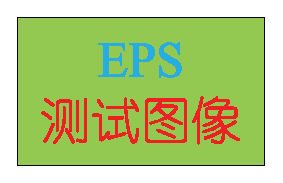
\includegraphics[width=0.3\textwidth]{chap2/testeps}}
%%%  \hspace{1in}
%%%  \subfigure[PDF Figure]{
%%%    \label{fig:epspdf:b} %% label for second subfigure
%%%    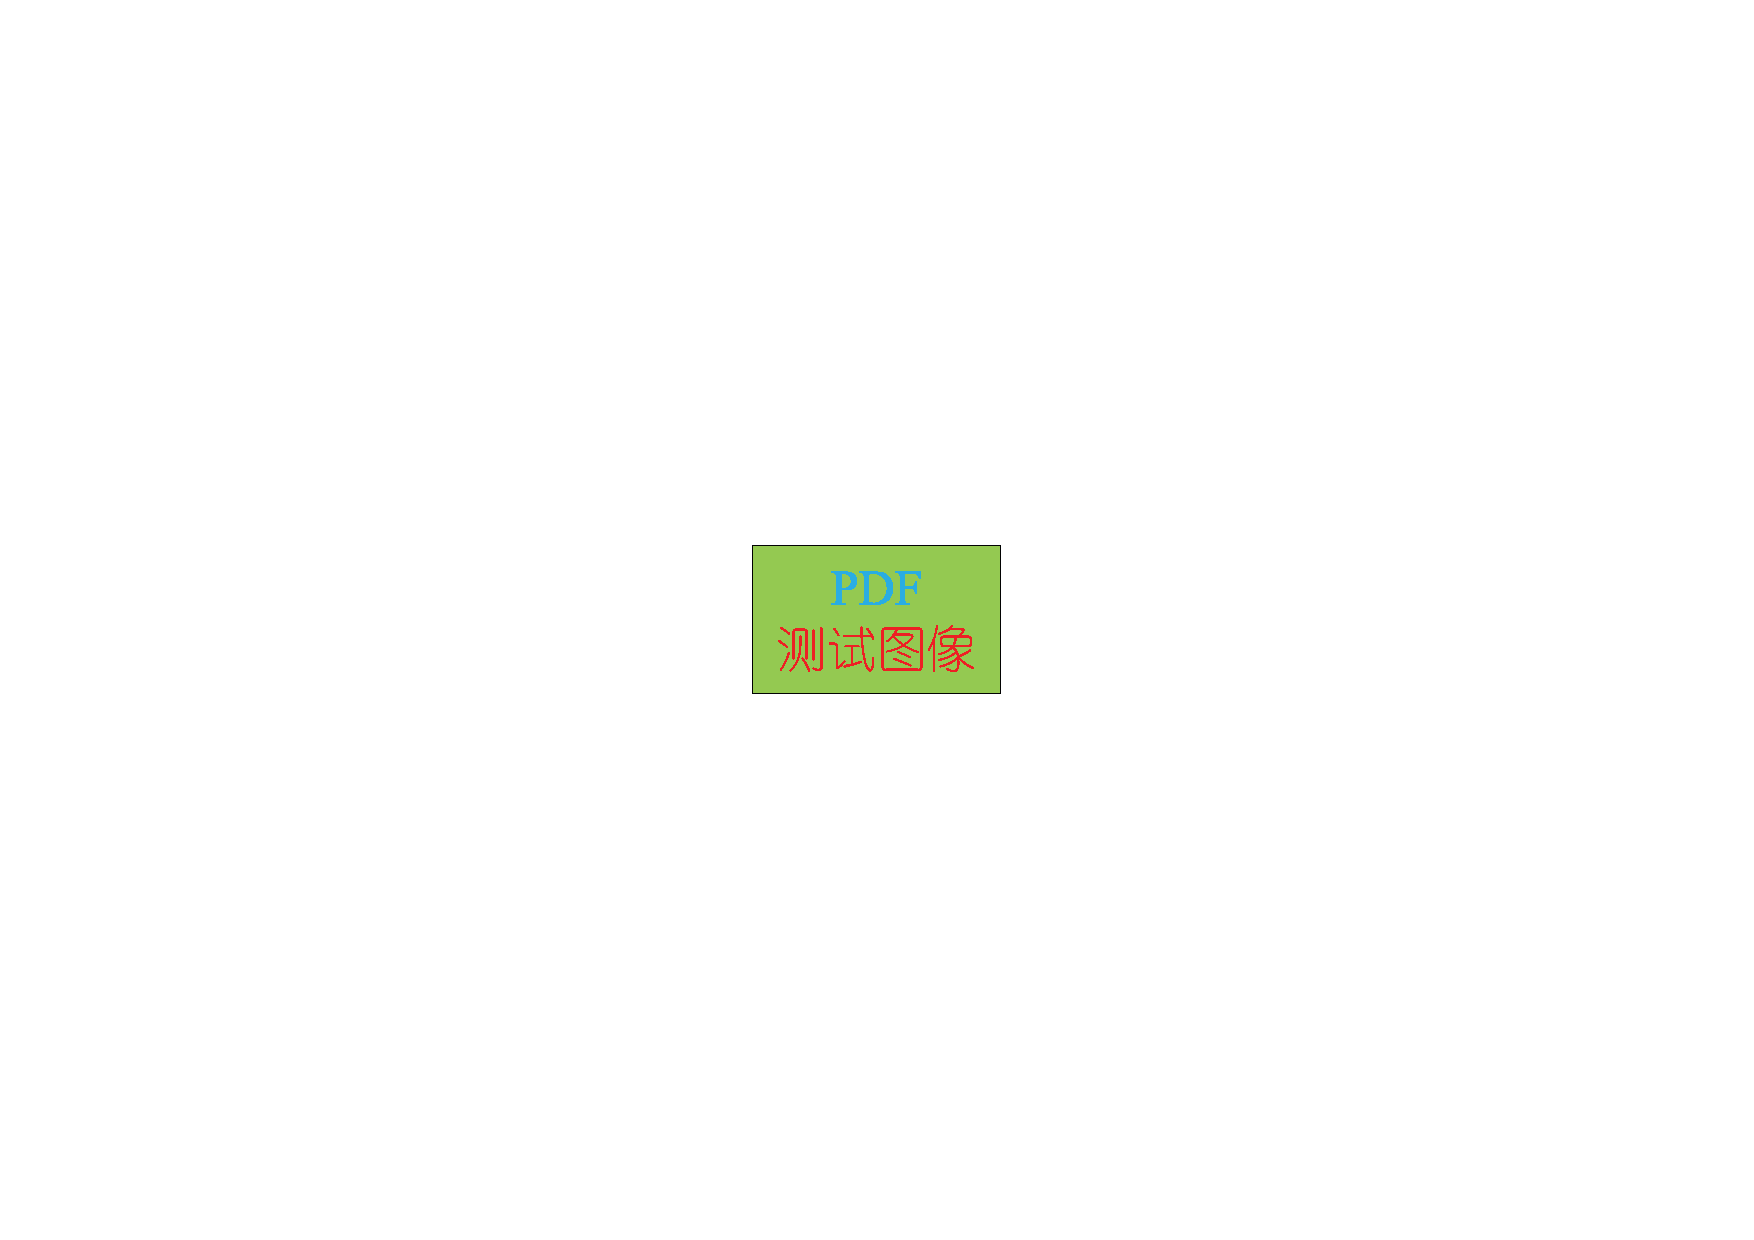
\includegraphics[angle=-90,origin=br,width=0.3\textwidth]{chap2/testpdf.pdf}}
%%%  \bicaption[fig:pdfeps]{插入eps图像和pdf图像}{插入eps和pdf的例子}{Fig}{An EPS and PDF demo}
%%%\end{figure}
%%%
%%%更多关于 \LaTeX 插图的例子可以参考\href{http://www.cs.duke.edu/junhu/Graphics3.pdf}{《\LaTeX 插图指南》}。
%%%
%%%\subsection{长标题的换行}
%%%\label{sec:longcaption}
%%%
%%%图\ref{fig:longcaptionbad}和图\ref{fig:longcaptiongood}都有比较长图标题,通过对比发现,图\ref{fig:longcaptiongood}的换行效果更好一些。
%%%其中使用了minipage环境来限制整个浮动题的宽度。
%%%
%%%\begin{figure}[!htp]
%%% \centering
%%% 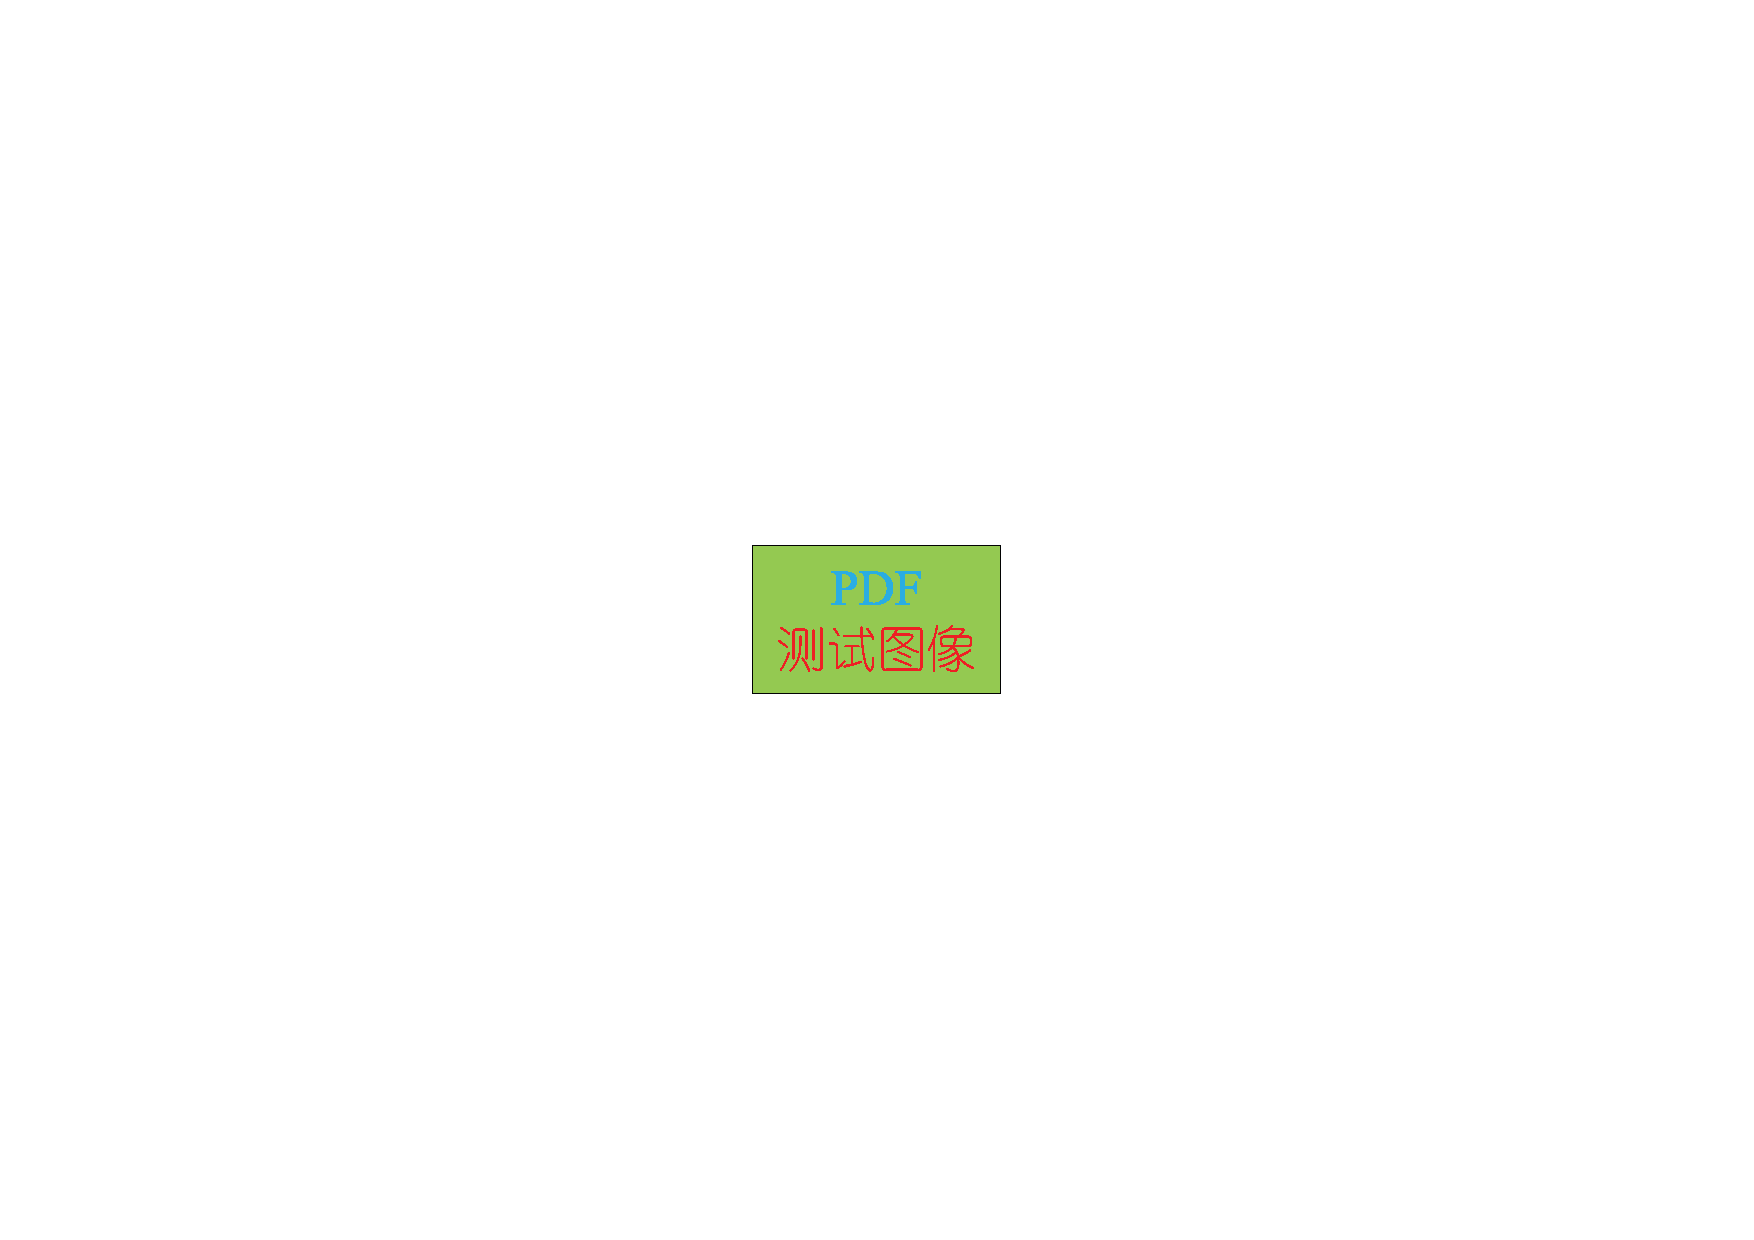
\includegraphics[angle=-90,origin=br,width=4cm]{chap2/testpdf.pdf}
%%% \bicaption[fig:longcaptionbad]{这里将出现在插图索引}{海交通大学是我国历史最悠久的高等学府之一,是教育部直属、教育部与上海市共建的全国重点大学.}{Fig}{Where there is a will, there is a way.}
%%%\end{figure}
%%%
%%%
%%%  \begin{figure}[!hbp]
%%%    \centering
%%%    \begin{minipage}[b]{0.6\textwidth}
%%%      \captionstyle{\centering}
%%%      \centering
%%%      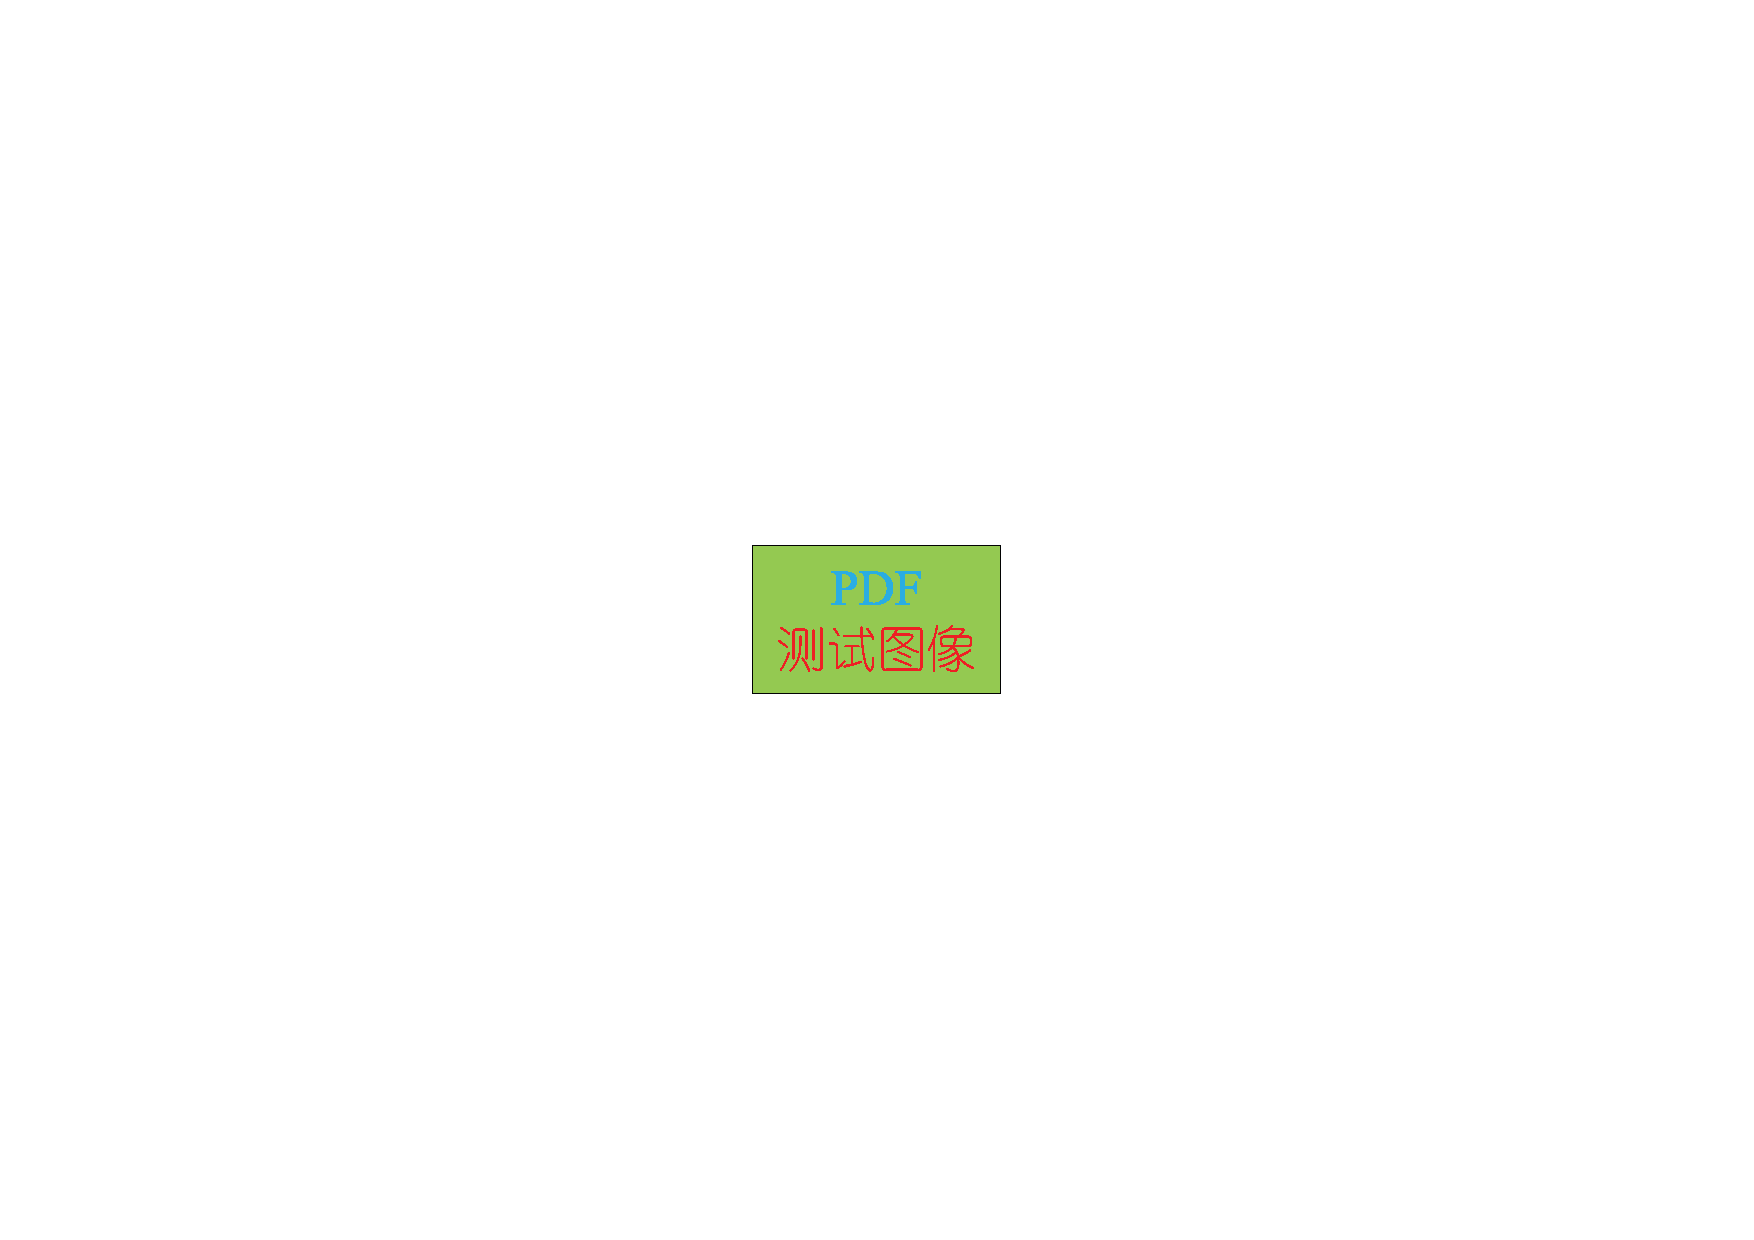
\includegraphics[angle=-90,origin=br,width=4cm]{chap2/testpdf.pdf}
%%%      \bicaption[fig:longcaptiongood]{这里将出现在插图索引}{海交通大学是我国历史最悠久的高等学府之一,是教育部直属、教育部与上海市共建的全国重点大学.}{Fig}{Where there is a will, there is a way.}
%%%    \end{minipage}
%%%  \end{figure}
%%%
%%%
%%%\section{表格的例子}
%%%\label{sec:tab}
%%%
%%%这一节给出的是一些表格的例子,如表\ref{tab:firstone}所示。
%%%
%%%\begin{table}[!hpb]
%%%  \centering
%%%  \bicaption[tab:firstone]{指向一个表格的表目录索引}{一个颇为标准的三线表格\footnotemark[1]}{Table}{A Table}
%%%  \begin{tabular}{@{}llr@{}} \toprule
%%%    \multicolumn{2}{c}{Item} \\ \cmidrule(r){1-2}
%%%    Animal & Description & Price (\$)\\ \midrule
%%%    Gnat & per gram & 13.65 \\
%%%    & each & 0.01 \\
%%%    Gnu & stuffed & 92.50 \\
%%%    Emu & stuffed & 33.33 \\
%%%    Armadillo & frozen & 8.99 \\ \bottomrule
%%%  \end{tabular}
%%%\end{table}
%%%\footnotetext[1]{这个例子来自\href{http://www.ctan.org/tex-archive/macros/latex/contrib/booktabs/booktabs.pdf}{《Publication quality tables in LATEX》}(booktabs 宏包的文档)。这也是一个在表格中使用脚注的例子,请留意与threeparttable实现的效果有何不同。}
%%%
%%%下面一个是一个更复杂的表格,用threeparttable实现带有脚注的表格,如表\ref{tab:footnote}。
%%%
%%%\begin{table}[!htpb]
%%%  \bicaption[tab:footnote]{出现在表目录的标题}{一个带有脚注的表格的例子}{Table}{A Table with footnotes}
%%%  \centering
%%%  \begin{threeparttable}[b]
%%%     \begin{tabular}{ccd{4}cccc}
%%%      \toprule
%%%      \multirow{2}{6mm}{total}&\multicolumn{2}{c}{20\tnote{1}} & \multicolumn{2}{c}{40} &  \multicolumn{2}{c}{60}\\
%%%      \cmidrule(lr){2-3}\cmidrule(lr){4-5}\cmidrule(lr){6-7}
%%%      &www & k & www & k & www & k \\
%%%      \midrule
%%%      &$\underset{(2.12)}{4.22}$ & 120.0140\tnote{2} & 333.15 & 0.0411 & 444.99 & 0.1387 \\
%%%      &168.6123 & 10.86 & 255.37 & 0.0353 & 376.14 & 0.1058 \\
%%%      &6.761    & 0.007 & 235.37 & 0.0267 & 348.66 & 0.1010 \\
%%%      \bottomrule
%%%    \end{tabular}
%%%    \begin{tablenotes}
%%%    \item [1] the first note.% or \item [a]
%%%    \item [2] the second note.% or \item [b]
%%%    \end{tablenotes}
%%%  \end{threeparttable}
%%%\end{table}
%%%
%%%\section{参考文献管理}
%%%
%%%参考文献的管理是这个学位论文模板又一个好玩的地方。
%%%
%%%\subsection{将参考文献的内容与表现分离}
%%%
%%%这个论文模板使用BibTeX处理参考文献,这又是一个``内容''与``表现形式''分离的极好例子
%%%\footnote{当然,你也可以手动编参考文献item,直接插入文档中。但是,有BibTeX帮助,我觉得没有人想用这种麻烦的方法,所以就在脚注中说明了。}。
%%%参考文献的``内容''就是reference文件夹下的chap\textit{xx}.bib,参考文献的元数据(名称、作者、出处等)以一定的格式保存在这些纯文本文件中。
%%%.bib文件也可以理解为参考文献的``数据库'',正文中所有引用的参考文件条目都会从这些文件中``析出''。
%%%控制参考文献条目``表现形式''(格式)的是.bst文件。.bst文件定义了参考文献风格,使用不同的参考文献风格能将同一个参考文献条目输出成不同的格式。
%%%当然,一个文档只能使用一个参考文献风格。
%%%按照教务处的要求,本模板使用的是国标GBT7714风格的参考文献。
%%%
%%%BibTeX的工作过程是这样的:
%%%BibTeX读取.aux(第一次运行latex得到的)看看你引用了什么参考文献条目,
%%%然后到.bib中找相关条目的信息,
%%%最后根据.bst的格式要求将参考文献条目格式化输出,写到.bbl文件中。
%%%在运行latex将.bbl插入文档之前,你可以用文本编辑器打开它,做一些小的修改。
%%%你会发现,.bbl的格式和你自己手动写item很相似,它已经被赋予了一定的``表现形式''。
%%%
%%%.bib数据库中的参考文献条目可以手动编写,也可以在google的学术搜索中找到。
%%%各大数据库\footnote{应该说是国际知名数据库,譬如SCOPUS, IEEE, OSA等,国内数据库在搜索、导出方面一直是差得一塌糊涂。}也支持将参考文献信息导出为.bib,
%%%省时省力。
%%%以Google学术搜索为例:进入\url{http://scholar.google.com},在``学术搜索设置''中,将`` 文献管理软件''设为``显示导入BibTeX''的连接,保存退出。
%%%然后学术搜索找到文献下会有``导出到BibTeX''连接,点击后Firefox会打开新的标签页,出现类似代码\ref{googlescholar}所示的内容
%%%\footnote{展示这些.bib条目使用了listings宏包,因为listings宏包协调中文的能力很糟糕,所以读者在查看模板的这部分源代码时会看到一些非常麻烦的东西。并且,直接将源代码的这部分内容复制到.bib中可能还会出错。我的建议是:这部分内容留意PDF就足够了。}。
%%%请注意,这个条目离``规范''还有一些距离。
%%%
%%%  \begin{lstlisting}[caption={从Google Scholar找到的,但并不规范的.bib条目}, label=googlescholar, float, escapeinside="", numbers=none]
%%%    @phdthesis{"白2008信用风险传染模型和信用衍生品的定价",
%%%      title={{"信用风险传染模型和信用衍生品的定价"}},
%%%      author={"白云芬"},
%%%      year={2008},
%%%      school={"上海交通大学"}
%%%    }
%%%  \end{lstlisting}
%%%
%%%  上面的.bib条目的``名字''\cndash{}``白2008信用风险传染模型和信用衍生品的定价'',包含ASCII以外的字符,BibTeX无法处理;
%%%  条目还缺少了address域,这样编译出来的结果会出现``地址不详'';
%%%  并且,条目还缺少language域,BibTeX需要language域来判断是否是中文参考文献。
%%%  将上面的条目修正(改英文名、增加address和language域),复制到本地的.bib文件中就可以了。
%%%  显然,这里描述的是参考文献的内容,而不是表现形式。
%%%
%%%  \begin{lstlisting}[caption={一个符合规范的.bib条目}, label=itemok, float, escapeinside="", numbers=none]
%%%    @phdthesis{bai2008,
%%%      title={{"信用风险传染模型和信用衍生品的定价"}},
%%%      author={"白云芬"},
%%%      year={2008},
%%%      language={zh},
%%%      address={"上海"},
%%%      school={"上海交通大学"}
%%%    }
%%%  \end{lstlisting}
%%%
%%%由于中英文参考文献处理起来有差异,所以需要在参考文献中标注是否是中文文献。
%%%确切地说,BibTeX并不具有区分中英文参考文献的``智能'',这种智慧的来源是.bst文——它定义了处理参考文献的规则。
%%%GBT7714-2005NLang.bst中规定:.bib中的条目,如果条目的``language''域非空,就被认为是中文文献,否则被认为是英文文献。
%%%例如,刚才的文献,就会被认为是中文参考文献,采取一些针对中文的处理方式。
%%%
%%%最后,这个条目被bibtex处理后,赋予了一定的``表现形式'',在.bbl文件中以下面的样子出现。
%%%你还可以对它进行小的修改,这是一种很折磨人的终极修改方法。
%%%再次运行latex之后,它将被插入到文档中。
%%%
%%%\begin{lstlisting}[caption={.bbl中被格式化之后的条目}, escapeinside="", numbers=none]
%%%\bibitem["白云芬(2008)"]{bai2008}
%%%  \textsc{"白云芬"}.
%%%  \newblock {"信用风险传染模型和信用衍生品的定价"}[D].
%%%  \newblock "上海: 上海交通大学, 2008."
%%%\end{lstlisting}
%%%
%%%再罗嗦两句,
%%%.bst文件书写起来非常繁杂\footnote{可以参考\href{http://ftp.ctex.org/mirrors/CTAN/info/bibtex/tamethebeast/ttb_en.pdf}{《Tame The BeaST》}。},书写符合GBT7714 标准的.bst文件更是一项浩大的工程。
%%%因此,当大家为漂亮、标准的参考文献列表感到满意时,应该对GBT7714-2005NLang.bst的作者充满谢意。
%%%作者在CTeX BBS发的帖子,请看
%%%\href{http://bbs.ctex.org/viewthread.php?tid=33571&highlight=\%B2\%CE\%BF\%BC\%CE\%C4\%CF\%D7\%2BGB}{文后参考文献著录规则 GB/T 7714-2005}。
%%%关于GB/T 7714-2005标准本身,请看\href{http://bbs.ctex.org/viewthread.php?tid=33571&highlight=GB\%2B\%B2\%CE\%BF\%BC\%CE\%C4\%CF\%D7}{这里}。
%%%
%%%再多说两句,.bib是“参考文献的内容”,而控制参考文献表现(格式)的是.bst文件,本模板附带的是GBT7714-2005NLang.bst。
%%%
%%%\subsection{在正文中引用参考文献}
%%%
%%%参考文献可以分章节管理,只需要在主文件中的参考文献中都包含进去就可以,如\verb+\bibliography{chap1,chap2,...}+。
%%%
%%%正文中引用参考文献时,用\verb+\upcite{key1,key2,key3...}+可以产生“上标引用的参考文献”,
%%%如\upcite{Meta_CN,chen2007act,DPMG}。
%%%使用\verb+\cite{key1,key2,key3...}+则可以产生水平引用的参考文献,例如\cite{JohnD,zhubajie,IEEE-1363}。
%%%请看下面的例子,将会穿插使用水平的和上标的参考文献:关于书的\cite{Meta_CN,JohnD,IEEE-1363},关于期刊的\upcite{chen2007act,chen2007ewi},
%%%会议论文\cite{DPMG,kocher99,cnproceed},
%%%硕士学位论文\cite{zhubajie,metamori2004},博士学位论文\upcite{shaheshang,FistSystem01,bai2008},标准文件\cite{IEEE-1363},技术报告\upcite{NPB2},电子文献\cite{xiaoyu2001, CHRISTINE1998},用户手册\cite{RManual}。
%%%
%%%最后总结一些注意事项:
%%%\begin{itemize}
%%%\item 参考文献只有在正文中被引用了,才会在最后的参考文献列表中出现;
%%%\item 参考文献``数据库文件''.bib是纯文本文件,请使用UTF-8编码,不要使用GBK编码;
%%%\item 参考文献条目中通过language域是否为空判断是否是中文文献;
%%%\item 参考文献条目同样有“内容”和“表现形式”之分,这种可控性是BibTeX带来的。
%%%\end{itemize}
%%%
%%%
%%%\subsection{参考文献管理器}
%%%
%%%参考文献数据库.bib虽然是纯文本的,可以用任意的文本编辑器查看,但总有人喜欢一个找一个``可视化''地查看每一条参考文献。
%%%我想\href{http://jabref.sourceforge.net/}{JabRef}应该是个很不错的选择。
%%%这是一个Java写的程序,需要JRE才能运行。
%%%就我测试的情况上看,很幸运,JabRef可以顺利打开GBK编码的.bib文件。
%%%但是,打开UTF--8编码的.bib源文件过程中总会崩溃,原因不得而知。
%%%由于我们的.bib文件使用的是UTF-8编码,所以JabRef暂时不可用。
%%%
%%%提到参考文献管理器,不得不提到另一个广被使用的软件——\href{http://www.endnote.com/}{EndNote}。
%%%在图书馆的宣讲会上,EndNote被吹得神乎其神,但我发现他对.bib的管理很不友好。
%%%EndNote可以导入.bib文件,却不能导出.bib,只能导出.bbl——被格式化的.bib。
%%%原来,JabRef比较``单纯'',不具备格式化参考文献的能力;
%%%而EndNote有那么一点设置参考文献输出格式的能力,然后就把这种能力滥用,这点搞得我很不爽。
%%%看来,EndNote和Word配合得更好一些。
%%%
%%%
%%%\section{用listings插入源代码}
%%%
%%%原先ctexbook文档类和listings宏包配合使用时,代码在换页时会出现莫名其妙的错误,后来经高人指点,顺利解决了。
%%%感兴趣的话,可以看看\href{http://bbs.ctex.org/viewthread.php?tid=53451}{这里}。
%%%这里给使用listings宏包插入源代码的例子,这里是一段C代码。
%%%另外,listings宏包真可谓博大精深,可以实现各种复杂、漂亮的效果,想要进一步学习的同学,可以参考
%%%\href{http://mirror.ctan.org/macros/latex/contrib/listings/listings.pdf}{listings宏包手册}。
%%%
%%%\begin{lstlisting}[language={C}, caption={一段C源代码}]
%%%#include <stdio.h>
%%%#include <unistd.h>
%%%#include <sys/types.h>
%%%#include <sys/wait.h>
%%%
%%%int main() {
%%%  pid_t pid;
%%%
%%%  switch ((pid = fork())) {
%%%  case -1:
%%%    printf("fork failed\n");
%%%    break;
%%%  case 0:
%%%    /* child calls exec */
%%%    execl("/bin/ls", "ls", "-l", (char*)0);
%%%    printf("execl failed\n");
%%%    break;
%%%  default:
%%%    /* parent uses wait to suspend execution until child finishes */
%%%    wait((int*)0);
%%%    printf("is completed\n");
%%%    break;
%%%  }
%%%
%%%  return 0;
%%%}
%%%\end{lstlisting}
%%%
%%%再给一个插入MATLAB代码的例子,感谢daisying站友提供的代码。
%%%
%%%\begin{lstlisting}[language={matlab}, caption={一段MATLAB源代码}]
%%%function paper1
%%%r=0.05;
%%%n=100;
%%%T=1;
%%%X=1;
%%%v0=0.8;
%%%sigma=sqrt(0.08);
%%%deltat=T/n;
%%%for i=1:n
%%%    t(i)=i*deltat;
%%%    w(i)=random('norm',0,t(i),1);
%%%end
%%%for i=1:n
%%%    alpha(i)=0.39;
%%%end
%%%for i=1:n
%%%    temp=0;
%%%    for k=1:i
%%%        temp=temp+alpha(k);
%%%    end
%%%    B(i)=exp(r*t(i));
%%%    BB(i)=B(i)*exp(temp*deltat);
%%%    BBB(i)=exp(-r*(T-t(i)));
%%%end
%%%for i=1:n
%%%    s0(i)=X*BBB(i);
%%%    v(i)=v0*exp((r-0.5*sigma^2)*t(i)+sigma*w(i));
%%%    for j=i+1:n
%%%        D=X*BBB(j);
%%%        d1=(log(v(i)/D)+(r+sigma^2/2)*(t(j)-t(i)))/(sigma*sqrt(t(j)-t(i)));
%%%        d2=d1-(sigma*sqrt(t(j)-t(i)));
%%%        ppp(i,j)=D*exp(-r*(t(j)-t(i)))*(1-cdf('normal',d2,0,1))-v(i)*(1-cdf('n
%%%ormal',d1,0,1));
%%%    end
%%%end
%%%for i=1:n
%%%    s1(i)=0;
%%%    for j=i+1:n
%%%        s1(i)=s1(i)+BB(j)^(-1)*alpha(j)*deltat*(X*BBB(j)-B(j)/B(i)*ppp(i,j));
%%%    end
%%%    s2(i)=0;
%%%    for j=1:n
%%%        s2(i)=s2(i)+alpha(j);
%%%    end
%%%    s2(i)=X*exp(-r*T-s2(i)*deltat);
%%%    s(i)=BB(i)*(s1(i)+s2(i));
%%%end
%%%plot(s)
%%%hold on;
%%%plot(s0);
%%%\end{lstlisting}

%%==================================================
%% chapter03.tex for SJTU Master Thesis
%% Encoding: UTF-8
%%==================================================

\chapter{抗信息泄露的可搜索加密}
\label{chap:searchpattern}

当前基于索引的可搜索加密方案都实现了云服务器中对加密数据进行检索的基本功能,并能获得Adaptive安全。基于正向索引的方案与使用反向索引技术的方案相比:正向索引方案中搜索效率与文档的数目成正比,而反向索引方案中搜索时间与文档大小无关仅为$O(1)$;两者方案都泄漏了大小模式和访问模式,而反向索引方案还泄漏了搜索模式而正向技术没有;但是,可搜索加密技术处于大数据的背景下,搜索时间是方案的一个重要指标,即使正向索引方案泄漏更少的信息,仍不被实际所采纳。

基于反向索引的可搜索加密技术的信息泄漏以curtmola\cite{curtmola2006searchable}中定义的trace --- 包括大小模式(size pattern)、搜索模式(search pattern)和访问模式(access pattern)为标准,即这些方案除了泄漏trace 信息之外,没有泄漏其它任何信息。至今为止,仍没有一个解决方案在实际上能抵御或降低该信息的泄漏。为此,从安全性角度出发,我们对以前方案进行了改进,提出了一个抗信息泄漏的可搜索加密方案。

通过使用史密斯正交化知识构建单词搜索陷门,使我们的方案在获得与通用可搜索方案有相同功能和安全的同时,避免了大小模式的泄漏,并分别仅以概率泄漏搜索模和访问模式,同时没有增加客户的负担和网络负荷。但是,该方案增加了服务器的存储开销和计算开销。

%%在本章中,我们提出了一个抗信息泄漏的可搜索加密方案。该方案在满足
%%以一定概率来泄漏可搜索加密环境中trace 信息泄漏的方案。首先,我们通过对文档进行预处理,从而避免了size pattern 的信息泄漏;然后我们以向量空间的知识对单词进行精心设计降低了search pattern 的泄漏;通过对文档和单词的处理工作同时也减少了access pattern 的泄漏问题;另外,我们方案中客户的计算和通讯开销的量级保持不变;最后,我们证明我们的方案中的信息泄漏比之前方案所泄漏的信息量小。但是,我们的方案显然增加了服务器的存储容量。

%%有如下特征:其搜索效率与文档的数目成正比,仅泄漏大小模式和访问模式没有泄漏搜索模式;而使用逆向索引的可搜索技术特征如下:搜索开销与文档大小无关仅为$O(1)$,泄漏了大小模式、访问模式和搜索模式。但是由于处在大数据的现实环境中,而不被广泛应用。

%实现当前基于逆向索引的可搜索加密的方案大多分别从功能和性能上进行扩展与优化,方案的安全性证明都是以curtmola 方案中trace 信息泄漏为基本前提。至今仍没有一个完整的解决方案从实际上能抵御trace 信息泄漏或以一种新的与trace对等的形式来衡量信息泄漏。为此,从方案的安全性考虑,必须提供一种能解决或者尽量减少trace 信息泄漏的办法。%Liu\cite{liu2014search} 等人虽然证明信息泄漏带来的问题,并使用一种简单的形式来描述如何避免trace的泄漏,但是因通讯和计算开销的增加太大而不能被实际使用。




\section{问题定义}
\label{sec:searchpattern_problem_definition}

在通用的可搜索加密模型\ref{fig:general_system_model}中,信息泄漏包括大小模式、访问模式和搜索模式,大小模式仅指文档的长度,很容易通过填充进行避免。下面我们分析搜索模式和访问模式,了解当前方案中导致该泄信息漏的根本原因。

\subsection{搜索模式泄漏}
\label{sec:searchpattern_problem_definition_search_pattern}
搜索模式是一个二维矩阵,其信息透露了该轮搜索的单词是否在之前已被搜索过。从图\ref{fig:general_system_model}我们可以了解到,搜索模式的泄漏主要来源于陷门生成函数使用的是确定性算法。如我们查询的单词序列是($w_1, w_2, w_1, w_1, w_1$),则请求的搜索陷门分别为($T_{w_1}, T_{w_2}, T_{w_1}, T_{w_1}, T_{w_1}$),这样敌手可以通过用户搜索习惯的统计信息并结合英文单词的频率推断出所查找的单词。另外,即使我们在搜索时的陷门使用概率算法没有泄漏,但是在建立索引时,若安全索引结构中每个单词的在查找表中的内容也是基于确定性的算法,则同样地敌手在查找过程中,通过查找表中匹配的结果来分析和推断出用户的搜索模式。因而,使用确定性的算法建立陷门必然会导致搜索模式的信息泄漏,我们必须设计一种新的算法来避免或以概率揭露用户的搜索模式给敌手。一个典型的搜索模式信息泄漏的情况如表\ref{tab3-1}所示:
 \begin{table}[h]
  \centering
  \begin{tabular}[t]{|c|c|}
  \hline
    文档 &       单词 \\
    \hline
    $w_1$ & $T(w_1)$ \\
    \hline
    $w_2$ & $T(w_2)$ \\
    \hline
    $w_3$ & $T(w_3)$ \\
    \hline
    $w_4$ & $T(w_4)$  \\
    \hline
  \end{tabular}
  \bicaption[tab3-1]{搜索模式信息泄漏示例}{搜索模式信息泄漏示例}
  {Table}{An Example Of Search Pattern Information Leakage}
  \end{table}

从上表可知,对于每个单词而言,他们所产生的陷门信息是确定的,即对同一单词必产生相同的输出陷门。为此,我们必须设计一个对某一个单词,其输出陷门是概率性确定的算法。
%在下面方案中,我们通过充分使用史密斯正交化理论的特点来巧妙地设计概率的单词陷门生成函数。



\subsection{访问模式泄漏}
\label{sec:searchpattern_problem_definition_access_pattern}
在$q$次查询历史的条件下,访问模式是指通过单词搜索得到$q$个密文文档的集合,即通过待查单词,敌手最终能获得查找后的文档结果集,即使不能解密,仍能通过多次的查找访问模式中概率推断出查找单词的搜索模式,若每个单词有唯一的文档ID集,则能完全推断。如已知5 次查询历史的单词为:$(w_1, w_2, w_3, w_2, w_1)$,敌手得到其对应的加密文档结果集,如图\ref{tab3-2} 所示:
\begin{table}[h]
  \centering
  \begin{tabular}[t]{|c|c|}
    \hline
    单词陷门 &       查找结果 \\
    \hline
    $T(w_1)$ & $c_1, c_3, c_4$ \\
    \hline
    $T(w_2)$ & $c_2, c_3, c_5$ \\
    \hline
    $T(w_3)$ & $c_1, c_2, c_5$ \\
    \hline
    $T(w_2)$ & $c_2, c_3, c_5$  \\
    \hline
    $T(w_1)$ & $c_1, c_3, c_4$  \\
    \hline
  \end{tabular}
  \bicaption[tab3-2]{访问模式信息泄漏示例}{访问模式信息泄漏示例}
  {Table}{An Example Of Access Pattern Information Leakage}
\end{table}

从表\ref{tab3-2}可知,对每一个单词,所对应的文档的结果集是唯一确定的。当搜索时,如果服务器发现该次查询在以前某次被查询过,服务器可以直接返回以前查询所记录的结果,而不管上次查询之后文档是否发生变化,这显然破环的方案的完整性,同时可以使用访问模式推断搜索模式。此外,如果访问模式没有被隐藏,即使搜索模式被隐藏了,我们同样可以通过访问模式以很大概率推导出搜索模式的信息。例如:5次查询历史仍为$(w_1, w_2, w_3, w_2, w_1)$,使用概率陷门生成算法后的结果如表\ref{tab3-3}所示:
\begin{table}[h]
  \centering
  \begin{tabular}[t]{|c|c|}
    \hline
    单词陷门 &       查找结果 \\
    \hline
    $T(w_1)$ & $c_1, c_3, c_4$ \\
    \hline
    $T(w_2)$ & $c_2, c_3, c_5$  \\
    \hline
    $T(w_3)$ & $c_1, c_2, c_5$  \\
    \hline
    $T(w_2')$ & $c_2, c_3, c_5$  \\
    \hline
    $T(w_1')$ & $c_1, c_3, c_4$  \\
    \hline
  \end{tabular}
  \bicaption[tab3-3]{改进后的访问模式信息泄漏示例}{改进后的访问模式信息泄漏示例}
  {Table}{An Example Of Improved Access Pattern Information Leakage}
\end{table}

从上表结果可知,我们仍然能通过搜索单词的结果集推断出:$T(w_1)$与$T(w_1')$和$T(w_2)$ 与$T(w_2')$ 是同一单词,虽然这个结果不是绝对的,但是敌手仍能以很大概率推断出多次搜索历史的Search Pattern。因此,仅仅隐藏搜索模式是显然不够的,同时必须在一定程度上隐藏访问模式。
%在这个方案中,我们以条件概率来泄漏方案的访问模式,但是不幸的是,该方式使服务器在存储开销上有所提升。


综上所述,为了完全隐藏方案中的trace信息,构造的方案必须具有以下特点:
\begin{enumerate}
  \item
  对于同一个单词,其对应的搜索陷门每次产生应该完全不相同,即敌手不能通过搜索陷门来推断出用户的搜索模式;并且搜索后,安全搜索的条目应有所变化,使得下次搜索时不能通过安全索引的已匹配项来推断出任何信息(如搜索模式);

  \item
  对于不同的单词,其对应的搜索陷门应该存在相同,即敌手不能通过输出的结果来推断用户的访问模式;同样地,对相同单词的多次搜索结果也应该有所不同;

  \item
  对于所有外包的文档的密文,它们的长度必须相等,以至于服务器在查询时不能通过长度来泄漏trace的大小模式。
\end{enumerate}

而在实际中,要实现具有上述特征的方案,必须查询时更新所有信息,这样的代价是不可取的。既然不可能完全掩盖trace的信息,我们只能尽可能地减少其信息的泄漏,即以条件概率来泄漏trace的信息量。


\subsection{前人的工作}
\label{sec:searchpattern_scheme_related_work}

Liu等人在方案\cite{liu2014search}中,首先证明了在通用的单关键字的可搜索加密方案中,敌手能利用少量的额外信息和用户的搜索模式发现用户搜索潜在的关键字。然后针对该问题,他们提出了一种基于分组的可搜索加密方案,该方案隐藏了搜索模式的泄漏,同时在一定程度上也避免了访问模式的泄漏,并通过实验证明了该方案的安全性。该方案由八个算法组成,其具体思路如下:
\begin{itemize}
  \item \textbf{$K \leftarrow KeyGen(1^\lambda).$}\ 方案使用安全参数$\lambda$,输出密钥$K$;

  \item \textbf{$I \leftarrow BuildIndex(D).$}\ 算法从文档集$D$中提取出单词与文档间索引关系$I$;

  \item \textbf{$(C, SI) \leftarrow Encryption(D,I,K).$}\ 该算法对文档加密和对明文索引$I$加密生成安全索引$SI$,并提交两者至服务器;

  \item \textbf{$S \leftarrow Dividing(k, W, V).$}\ 该算法使用参数$k$、$W$和$V$ (其中$k$表示对单词集分组后每组的元素个数,$W$是文档中所有不同单词的集合,$V$表示额外的知识,被数据所有者和敌手所使用),输出分组的单词集$S$,过程如下:
      \begin{enumerate}
        \item 根据$V$的频率分布,将单词集$W$排序;
        \item 将排序后的单词集分成$|W|/k$组,每组$k$个元素:$S = (S_1, S_2, ...,S_{|W|/k})$;
        \item 将每组的元素$S_i$($1 \leq i \leq |W|/k$)用洗牌算法对其进行重排。
      \end{enumerate}

  \item \textbf{($b, \mathcal{Q}) \leftarrow Query(k, w, K, S).$}\ 用户查询单词$w$,调用算法$Dividing$对单词进行重新分组。然后从分组的集合$S$中,查询得到包含单词$w$的集合$S_q$;对集合$S_q$ 中第$i$ 个单词建立陷门$sq_i$,记$\mathcal{Q} = \{sq_1, ..., sq_k\}$,并记录单词$w$ 在集合中的位置记为$b$和更新额外信息$V$;保存$b$在用户端,并提交请求$\mathcal{Q}$;

  \item \textbf{$R \leftarrow Search(\mathcal{Q}, SI).$}\  服务器收到请求$\mathcal{Q}$后,对每个元素元素$\mathcal{Q}[i]$查询得到结果集$R_i$,并返回结果集$R = \{ R_1, ..., R_k \}$;

  \item \textbf{$R_b \leftarrow Extract(R,b).$}\ 请求者收到结果集后,根据请求单词所在位置$b$,提取出目的结果$R_b$;

  \item \textbf{$D_i \leftarrow Decryption(C_i, K).$}\ 用户使用文档加密密钥$K$解密$R_b$:$D_i \leftarrow SKE.Dec(C_i, K)$($C_i \in R_b$)。

\end{itemize}

该方案的缺陷在于:(1)需要了解并利用额外的知识$V$,在某些情况下,这个限制条件是很难达到的;(2)客户需要存储分组后的单词集合$S$,并且需要维持集合$S$的内容在不同授权用户之间的一致性问题;(3)服务端返回的结果非常大,包括所有请求的单词的结果$R$,导致网络间的通讯量是所需答案信息量的$k$倍,同时也增加了服务端的计算开销,与分组中每组的单词个数$k$ 密切相关。当$k$ 足够大时,计算和存储开销太大,当$k$ 很小时,不容易隐藏用户的搜索模式。因而如何选择常数也成了本方案的关键。并且在该方案中,如果不每次更新集合$S$,如:查询单词$(w_1, w_2, w_1, w_1, w_1)$,请求陷门如下:
\begin{flushleft}
\[
  \begin{cases}
   \mathcal{Q}_1 & \text{= } \{ sq(w_7), sq(w_1), sq(w_{15}) \} \\
   \mathcal{Q}_2 & \text{= } \{ sq(w_2), sq(w_6), sq(w_8)    \} \\
   \mathcal{Q}_3 & \text{= } \{ sq(w_7), sq(w_1), sq(w_{15}) \} \\
   \mathcal{Q}_4 & \text{= } \{ sq(w_7), sq(w_1), sq(w_{15}) \} \\
   \mathcal{Q}_5 & \text{= } \{ sq(w_7), sq(w_1), sq(w_{15}) \}
  \end{cases}
\]
\end{flushleft}

从上例可知,服务器通过对上述多次请求陷门集合进行比对,照样推断出用户的搜索模式。因而,在每次查询时,都必须对单词集进行重新分组,以避免search pattern的泄漏。对上例重新分组后的可能结果如下:
\begin{flushleft}
\[
  \begin{cases}
   \mathcal{Q}_1 & \text{= } \{ sq(w_7), sq(w_1), sq(w_8) \} \\
   \mathcal{Q}_2 & \text{= } \{ sq(w_2), sq(w_6), sq(w_8) \} \\
   \mathcal{Q}_3 & \text{= } \{ sq(w_7), sq(w_1), sq(w_2) \} \\
   \mathcal{Q}_4 & \text{= } \{ sq(w_1), sq(w_7), sq(w_2) \} \\
   \mathcal{Q}_5 & \text{= } \{ sq(w_2), sq(w_1), sq(w_7) \}
  \end{cases}
\]
\end{flushleft}
通过这样的改变,服务器显然不能推断出用户的搜索模式。

Islam等人在方案\cite{islam2012access}中,提出一个新颖的攻击模型,该模型利用泄漏的访问模式和先验知识来推断用户某些敏感的信息。然后针对该攻击,提出了一个避免access pattern泄漏的方案。但是,该方案引入了误报率和增加通讯开销。方案思路如下:
\begin{itemize}
  \item \textbf{建立索引:}在该阶段,用一个$m*n$的二维矩阵$ID$来存储安全索引($m$---单词数目,$n$ --- 文档数目),元素$ID_{i,j}$ 表示单词$w_i$是否在文档$D_j$中,若在为1,否则为0。建立阶段,每行元素通过如下方式构建:对该单词包含在某文档中的位置必置为1,否在在其它非1位置随机选择几个置为1。 然后使用近似算法将$ID$ 转化为安全的矩阵索引;

  \item \textbf{查询结果:}在查找阶段,对安全索引进行查找,返回所有符合条件的结果。
\end{itemize}
显然,在该方案中,引入了一定的误报率,并且要构造如此的近似函数也不是易事;同时,在搜索结果中通过错误的结果增加了传输的通讯开销。


%%\section{系统模型}
%%\label{sec:searchpattern_model}

\section{方案框架}
\label{sec:searchpattern_scheme_framework}


\subsection{方案相关定义}
\label{sec:searchpattern_scheme_related_definition}

%%在我们的方案中,为了减少Trace的信息泄漏,我们使用基于向量空间的史密斯正交化原理来避免搜索模式的信息泄漏。下面介绍一些相关定义和方案中所使用的符号说明。

%%%%%%%%%%%%%%%%%%%%%%%%%%%%%%%%%%%%%%%%%%%%%%%%%%%%%%%%%%%%%%%%%%%%
%\begin{defn}[向量内积(Inner Scalar Product)]
%\label{defn:scale_function}
%如果一个函数$\phi$在$n$维空间上有:
%\begin{center}
%$ \{0, 1\}^n \times \{0, 1\}^n \rightarrow \mathcal{[}0,n\mathcal{]} $,
%%$\phi$ : $x$ $\ast$ $y$ $\rightarrow$ $\sum_{i=1}^{n}(x_i y_i)$ \ \ ($x = (x_1, ..., x_n), y = (y_1, ..., y_n)$, $x_i, y_i$ $\leftarrow$ $\{0,1\}^{n}$ ),
%\end{center}
%则称函数$\phi$是向量的内积函数(简称向量内积)。
%\end{defn}
%%%%%%%%%%%%%%%%%%%%%%%%%%%%%%%%%%%%%%%%%%%%%%%%%%%%%%%%%%%%%%%%%%%%


%%%%%%%%%%%%%%%%%%%%%%%%%%%%%%%%%%%%%%%%%%%%%%%%%%%%%%%%%%%%%%%%%%%%%%
\begin{defn}[正交投影]
\label{defn:scale_function}

在相同空间中,向量$v$在向量$u$上的正交投影$p$,定义为:
\begin{center}
$p_u(v) = \frac{\phi(u,v)}{\phi(u,u)} u$
\end{center}
\end{defn}
$\phi$是一个向量内积函数。

%%%%%%%%%%%%%%%%%%%%%%%%%%%%%%%%%%%%%%%%%%%%%%%%%%%%%%%%%%%%%%%%%%%%%%


%%%%%%%%%%%%%%%%%%%%%%%%%%%%%%%%%%%%%%%%%%%%%%%%%%%%%%%%%%%%%%%%%%%%%%
\begin{thm}[Gram-Schmidt]
\label{thm:gram_schmidt}
如果$(f_i)_{i\in\{0,n\}}$是一个pre-Hilbert向量空间系,$\phi$是一个向量内积函数,则必存在一个正交系$(o_i)_{i\in\{0, l\}}$ 使:
\begin{itemize}
  \item $\phi(o_i, o_j) = \phi(o_i, o_i)\delta_{i,j}$,
  \item $Vect(f_1,..., f_l) = Vect(o_1, ...o_l)$,
  \item 标量积$\phi(f_i,o_i)$严格为正。
\end{itemize}
\end{thm}
%%%%%%%%%%%%%%%%%%%%%%%%%%%%%%%%%%%%%%%%%%%%%%%%%%%%%%%%%%%%%%%%%%%%%%




\begin{tabular}{|| l || l ||}
  \hline
  % after \\: \hline or \cline{col1-col2} \cline{col3-col4} ...
  Notations & Explanations \\
  \hline
  $p$     & 常量,对每个文档块复制$p$份 \\
  $q$     & 常量,对每个单词构造$q$个相关联的向量 \\
  $m$     & 常量,将每个文档分成$m$块 \\
  $T$     & 查找表,存储单词陷门内容 \\
  $A$     & 数组,存储所有单词的文档$ID$信息 \\
  $A_d$   & 数组,存储加密文档的数据块 \\
  $D$     & 集合,所有的文档 \\
  $W(D) $    & 数组,文档集$D$中所有不同的单词集合 \\
  $ID(w)$    & 数组,所有包含单词$w$的文档的$ID$ \\
  $A[i] $    & 数组中第$i$个元素 \\
  \hline
\end{tabular}


%%\begin{itemize}
%%  \item \textbf{p} ---
%%
%%  \item \textbf{q} ---
%%
%%  \item \textbf{} ---
%%
%%  \item \textbf{} ---
%%
%%  \item \textbf{} ---
%%
%%  \item \textbf{} ---
%%
%%\end{itemize}

\subsection{方案框架}
\label{sec:searchpattern_scheme_description}

在不可信的云环境下,我们实现了一个抗信息泄漏的可搜索加密方案。我们的系统模型与通用的系统模型\ref{fig:general_system_model}相同,包括数据拥有者、被授权的用户和云服务提供商。数据拥有者负责数据的初始化和安全索引的构建,用户搜索并解密所需文档,而云服务提供商提供存储外包服务和遵照用户规则对外包数据进行检索并返回结果。方案思想如下:
\begin{enumerate}
  \item 在建立索引阶段,对每个单词的处理如下:将每个单词转换向量;

  \item 在查找阶段,单词查找口令按如下方式生成:将该单词按同样方式生成向量$V$,然后构建向量的法平面,取法平面内的任意向量,由法平面内的任一向量与向量$V$垂直(),可构造出类似的概率算法。
\end{enumerate}

该方案由七个算法组成,如下所示:
\begin{itemize}
  \item \textbf{密钥生成:}数据所有者使用安全参数,生成解密文档和建立索引所需要的密钥;

  \item \textbf{文档加密:}数据拥有者对将上传的文档分块、加密并建立各块之间的联系,对每篇文档生成一个链表,同时使服务器能通过起始块恢复出完整的文档;

  \item \textbf{安全索引建立:}数据所有者提取待上传的文档的关键字信息,对关键字建立安全索引,并建立安全索引与加密文档之间的关联;
 
  \item \textbf{外包:}数据所有者将安全索引和加密文档上传至云服务器;

  \item \textbf{陷门生成:}当被数据拥有者授权的用户想要查找包含某单词的文档时,调用安全陷门生成函数计算单词的陷门,发送给服务器;

  \item \textbf{搜索:}一旦云服务器收到用户所提交的单词查找陷门时,使用单词陷门在安全索引上检索得到文档$ID$,通过文档$ID$查找获得文档首块地址,按首块地址得到文档的所有块,回送给用户;

  \item \textbf{解密:}用户对收到的所有加密文档块进行解密,扔掉无用的块和恢复出完整的文档。
\end{itemize}



\section{方案细节}
\label{sec:searchpattern_scheme}

在已有方案和技术的基础上,我们构造了一个抗信息泄漏的可搜索加密方案,该方案具有如下特征:没有泄漏大小模式,仅以概率泄漏访问模式和搜索模式,并与已有方案有相同的安全级别。

%%%%%%%%%%%%%%%%%%%%%%%%%%%%%%%%%%%%%%%%%%%%%%%%%%%%%%%%%%%%%%%%%%%%%%
\begin{defn}[抗信息泄漏的可搜索加密方案]
\label{defn:resist_trace}
该方案包括七部分:($Setup$,$DEnc$,$BuildSIndex$,$Outsource$,$TrapdrGen$,$Query$,$Dec$),其数学描述如下:
\begin{itemize}
  \item \textbf{$K \leftarrow Setup(1^k)$.}\ 方案中该算法是简单的密钥生成函数。单词加密密钥从$\{0,1\}^k$中随机取样,文档加密密钥调用$SKE.KeyGen(1^k)$生成,生成包括加密文档和建立安全索引的密钥$K$;
将每个文档
  \item \textbf{$A_d \leftarrow DEnc(D, K)$.}\ 该算法使用参数$D$和$K$对文档进行分块,分别加密并存放至数组$A_d$中且维护各块之间的关联;

  \item \textbf{$I \leftarrow BuildSIndex(D, K)$.}\ 索引建立算法使用参数$D$和密钥$K$,提取文档中单词$W(D)$并建立安全索引同时维持单词与文档之间的关系,即通过单词能快速定位到包含单词的文档$ID$;

  \item \textbf{$Outsource(A_d, I)$.} 该过程仅仅将加密的结果$A_d$和$I$外包至远程的服务器;

  \item \textbf{$T_w \leftarrow TrapdrGen(w, K)$.}\ 陷门生成函数是一个概率算法。主要由授权的用户所调用,用于生成查询陷门。在该方案中,算法使用同一单词$w$和$K$,但每次输出不同的陷门$T_w$;

  \item \textbf{$R \leftarrow Query(w, I, A_d)$.}\ 该过程是确定性的查询算法,包括使用单词陷门对安全索引进行查找获得所有文档的首块地址,然后通过该地址对文档信息进行查找获得完整的文档块结果集合$R$,并返回;

  \item \textbf{$PD \leftarrow Dec(R, K)$.}\ 是确定性的解密算法,对收到的$R_i \in R$中的每块调用算法$SKE.Dec$进行解密,并将解密的各块连接起来形成完成的文档$PD$,即为正确的文档。
\end{itemize}
\end{defn}
%%%%%%%%%%%%%%%%%%%%%%%%%%%%%%%%%%%%%%%%%%%%%%%%%%%%%%%%%%%%%%%%%%%%%%

从上述定义可知,$Setup$是简单的密钥生成算法,$Outsource$仅仅将数据外包,这两个算法与其它方案中算法一致,无改进之处。下面分四个过程(加密、陷门生成、查询和解密)对其它算法进行描述。其中,加密包括对文档$D$进行加密和建立查找结构$I$。

\subsection{加密}
\label{sec:searchpattern_scheme_encryption}


首先数据所有者调用密钥生成函数$Setup$生成密钥$K = (K_1, K_2, K_3, K_4, SK_1,$ $..., SK_p)$;用于对文档进行加密和建立安全索引。

\textbf{文档加密($DEnc$)} 首先对所有文档$D=(D_i, ..., D_n)$进行填充,使所有文档具有相同的大小。然后将每个文档$D_i \in D$划分成$m$个大小相同的块$D_i = (B_1 , ... , B_m)$,并在每个文档块的后面加一个代表该块所在文件中位置的标记,如加上标记后的文件块为:$B = (B_1||1, ..., B_m||m)$;紧接着,将标记后的文件块复制$p$份并随机洗牌,然后对每块分别用加密函数$SKE.Enc$和密钥$SK_i$ 进行加密,加密后放入数组$A_d$ 中,并将所有的块用一个链连接起来,第$i$个数据块在数组$A_d$ 结点中的信息如下:
\begin{center}
$A_d[addr_{D}(B[i])] = <SKE.Enc_{SK_i}(B_i||i), addr_{D}(B[i+1])>$,
\end{center}

这里$addr_{D}(B[i])$ --- 表示$B$中第$i$块在数组$A_d$中的地址。若取$p$=2,将每个文档分成三块,则在数组$A_d$中对每个文档分块并加密建立关联后的结构如图\ref{fig:file_block_list}所示:
\begin{figure}[!htp]
  \centering
  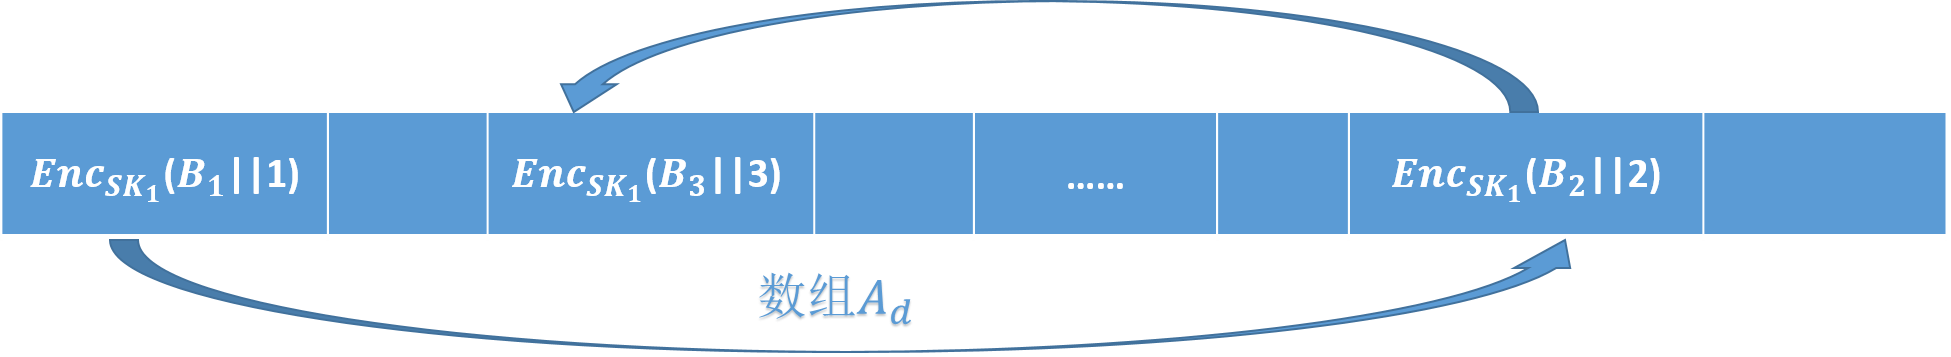
\includegraphics[width=0.95\textwidth]{chap3/file_list}

  \bicaption[fig:file_block_list]{加密后文档块链表}{加密后文档块链表} {Fig}{Document Block List of Encryption}
\end{figure}


\textbf{索引建立($BuildSIndex$)} 首先对所有文档集$D$,提取出$D$中所有不同的单词集合$W(D) = \{w_1, ..., w_{|W(D)|} \}$;然后对每个单词$w_i \in W(D)$,使用伪随机置换函数 $\pi_{K_1}$生成一个置换后的单词集合$PW = \{\pi_{K_1}(w_1), ..., \pi_{K_1}(w_{|W(D)|} \}$。

随后,我们选取$|W(D)|$个$l-2$ 维的标准化正交基(正交基的建立过程可以使用史密斯正交化理论构建
\cite{daniel1976reorthogonalization}):$\{e_1, ..., e_{|W(D)|}\}$ ,$|e_i| = l-2$,$i \in [1, |W(D)|]$;然后将每个置换后的单词与对应的正交基拼接起来,则每个单词$w_i$的结构如下:$\pi_{K_1}(w_i) || e_i$,且每个结构的大小为$l-1$ 维;再分别将集合$[1,q]$中每个数与变化后的单词结构相连接,则最终对每个单词$w_i$形成$q$个$l$ 维的空间向量,对$1 \leq i \leq |W(D)|$ 和$1 \leq j \leq q$,其结构为$f_{w_i,j} = (\pi_{K_1}(w_i) || e_i || j)$。
对每个变量$f_{w_i,j}$,使用伪随机函数$F_{K_2}$生成一个结果放入查找表(look-up)$T$中,在$T$中每个结点存储的内容如下:
\begin{center}
    $T[F_{K_2}(f_{w_i,j})] = <f_{w_i,j}, addr_{ID}(ID(w_i)[1])> \oplus \mathcal{G}(P_{K_3}(f_{w_i,j}))$,
\end{center}
这里$F_{K_2}$和$P_{K_3}$是伪随机函数,$\mathcal{G}$是伪随机生成器,$addr_{ID}(ID(w_i)[1])$是指单词$w_i$所对应的文档$ID$集合在文档$ID$数组$A$中的第一个文档ID所存放的地址。


对每个单词$w_i \in W(D)$,建立文档$ID$的集合$ID(w_i) = \{ID(D_i) | w_i \in D_i \}$,并填充是所有的集合$|W(D)|$大小相等;然后对每个$ID(w_i$建立链表$L_{w_i}$,使之在$ID(w_i)$中每个元素($1 \leq j \leq |ID(w_i)|$)在数组$A_s$ 中的结构如下:
\begin{center}
$A[addr_{ID}(ID(w_i)[j])] = (<ID(w_i)[j], addr_{ID}(ID(w_i)[j+1])> \oplus H(Q_{K_4}(f_{w_i,j}),r_i), r_i)$,
\end{center}
这里$r_i$ --- 随机字符串,$ID(w_i)[j]$ --- 表示集合$ID(w_i)$中的第$j$个元素,$addr_{ID}(ID(w_i)[j])$ --- 表示元素$ID(w_i)[j]$存放在数组$A$中的地址,$Q_{K_4}$ --- 表示伪随机函数,$H$ --- 表示伪随机置换。

如$q = 2$,对包含三个单词的文档,按照上述方式,构建完成后的安全索引结构如下图\ref{fig:resist_secure_index} 所示:
\begin{figure}[!htp]
  \centering
  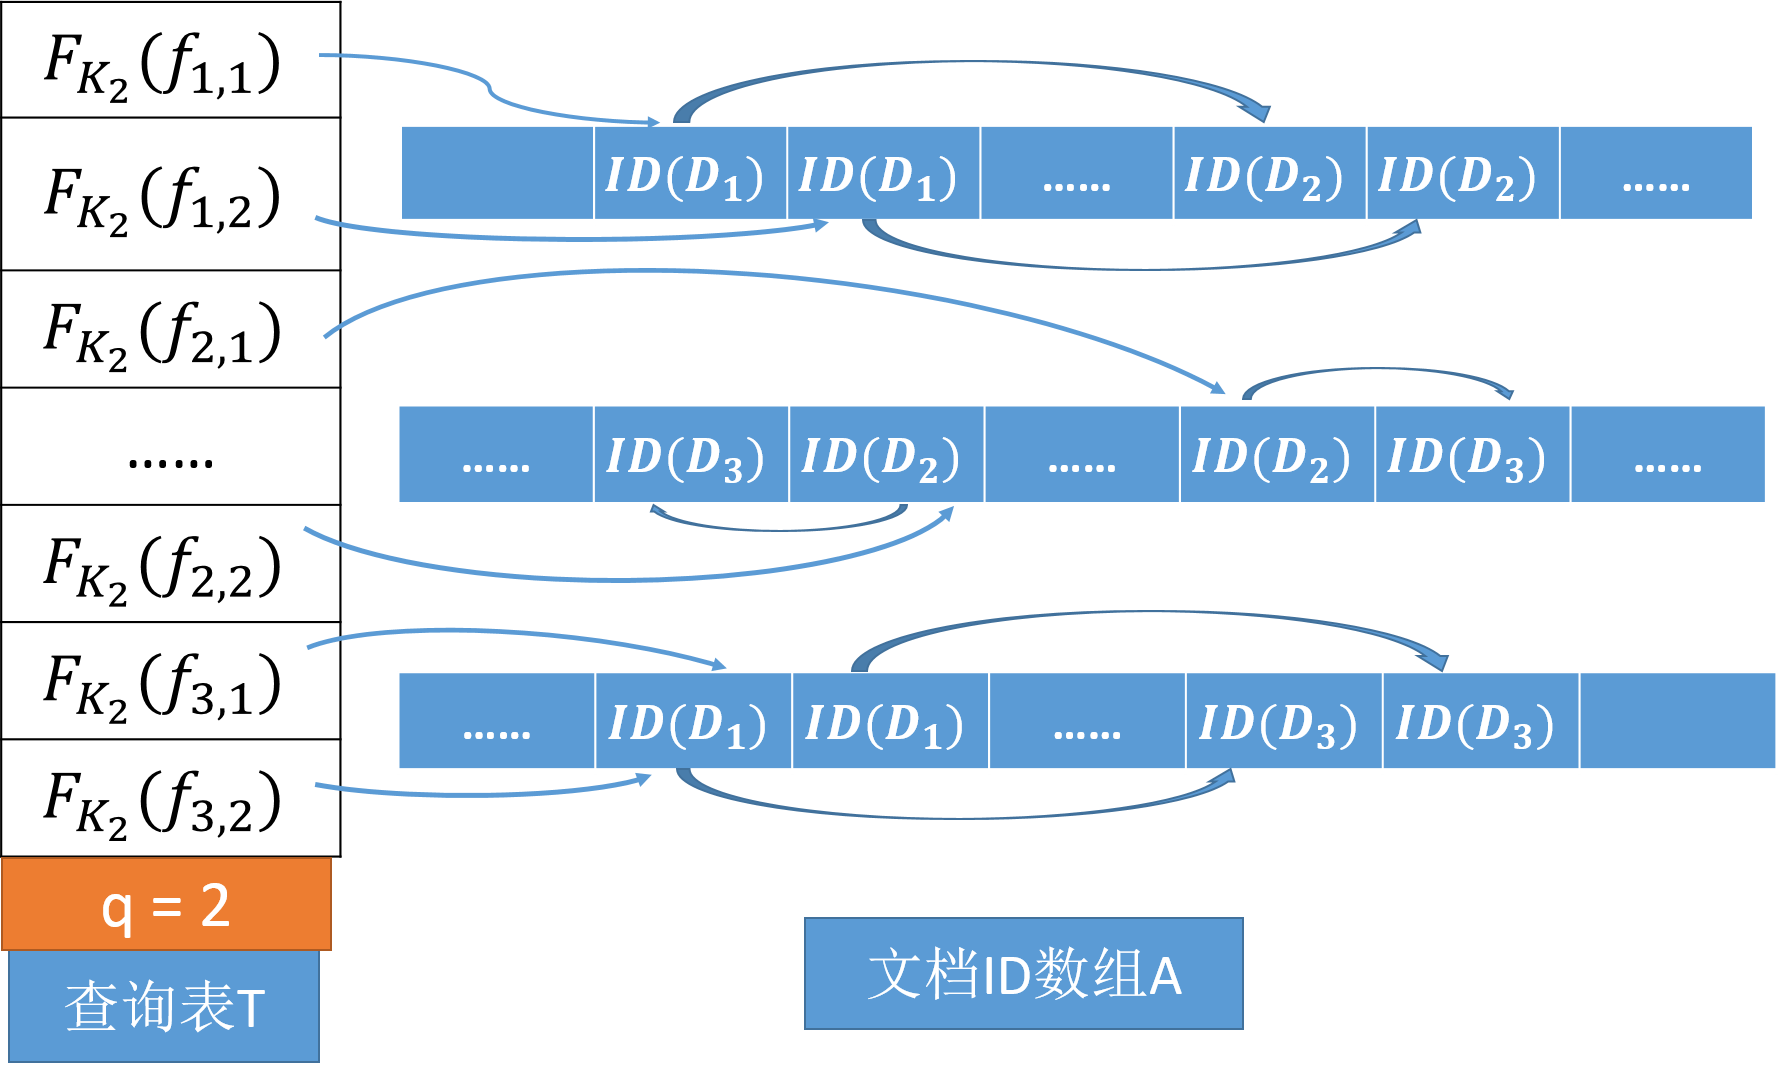
\includegraphics[width=0.95\textwidth]{chap3/resist_secure_index}

  \bicaption[fig:resist_secure_index]{抗泄漏方案的安全索引}{抗泄漏方案的安全索引} {Fig}{Secure Index of Resisting Information Leakage}
\end{figure}

数据拥有者在加密过程中主要使用了两个函数:文档加密函数$DEnc$ \ref{alg:DEnc}和安全索引建立算法$BuildSIndex$ --- 包括两个子算法:$BuildLookup$ \ref{alg:BuildLookup}与$BuildArray$ \ref{alg:BuildArray},其具体实现过程分别如下:

%%
%%  algorithm: DEnc
%%
\begin{algorithm}[!htb]
\caption{$A_d \leftarrow DEnc(D, K)$}
\label{alg:DEnc}
\begin{algorithmic} [1]

\ENSURE ~~\\
  \COMMENT{ \textbf{Initialization}} ~~\\
         allocate enough array: $A_d$ ~~\\
         make each $|D_i|$ equal by filling ~~\\
  \COMMENT{ \textbf{Build List for $D$}} ~~\\
  \STATE divide each $D_i \in D$ into m blocks:$D_i = (B_1, ..., B_m)$
  \STATE add unique location flag to $D_i$, get: $B$ =($B_1||1, ..., B_m||m$)
  \STATE make $p$ copies of $B$, and randomly shuffle for each one 
         \FOR {$1 \leq j \leq p$}
           \FOR { $B_i \in B$}
              \STATE create a node: $A_d[addr_D(B_i)] = < SKE.Enc_{SK_j}(B_i), addr_D(B[i+1]) >$,
                     where $addr_D(B_i)$ is randomly unique address. ~~\\
                     for the last block, having: $addr_D(B_m) = NULL$ ~~\\
           \ENDFOR
         \ENDFOR
  %
  % RETURN VALUE OF THE ALGORITHMS
  %
  \RETURN ${A_d}$;

\end{algorithmic}
\end{algorithm}

%%
%%  algorithm: BuildLookup
%%
\begin{algorithm}[!htb]
\caption{$T \leftarrow BuildLookup(D,K)$}
% algorithm label to be referred in the text
\label{alg:BuildLookup}
\begin{algorithmic} [1]

\ENSURE ~~\\
  \COMMENT{ \textbf{Initialization}} ~~\\
  \STATE allocate enough look-up table $T$ ~~\\
         select orthogonal basis $\{e_1, ..., e_{|W(D)|} \}$ of $l-2$ dimensions ~~\\
         randomly select constant $q$ ~~\\
  \COMMENT{ \textbf{Build Look-up Table $T$}} ~~\\
         \FOR {$w_i \in W(D)$}
           \STATE generate: $t(w_i) = \pi_{K_1}(w_i) || e_i$, $|t(w)| = l-1$
           \FOR {$1 \leq j \leq q$}
             \STATE get: $f_{w_i,j} = t(w_i) || j$ ~~\\
             \STATE for $f_{w_i,j}$, create a node: ~~\\
                    $T[F_{K_2}(f_{w_i,j})] = <f_{w_i,j}, addr_{ID}(ID(w_i)[1])> \oplus \mathcal{G}(P_{K_3}(f_{w_i,j}))$

           \ENDFOR
         \ENDFOR
         \STATE fill remaining blanks to random value.
  %
  % RETURN VALUE OF THE ALGORITHMS
  %
  \RETURN ${T}$;
\end{algorithmic}
\end{algorithm}

%%
%% algorithm: BuildArray
%%
\begin{algorithm}[!htb]
\caption{$A \leftarrow BuildArray(D,K)$}
\label{alg:BuildArray}
\begin{algorithmic} [1]

\ENSURE ~~\\
  \COMMENT{ \textbf{Initialization}} ~~\\
  \STATE get $ID(w_i)$ of $w_i \in W(D)$ ~~\\
         assure all $|ID(w_i)|$ equal ~~\\
         allocate enough array $A$ ~~\\
  \COMMENT{ \textbf{Build Array $A$}} ~~\\
         \FOR {$w_i \in W(D)$}
           \FOR {$1 \leq j \leq |ID(w_i)$}
             \STATE create a node in $A$:  \ \ $A[addr_{ID}(ID(w_i)[j])] = $ ~~\\
                    $<ID(w_i)[j], addr_{ID}(ID(w_i)[j+1])> \oplus \mathcal{H}(Q_{K_4}(f_{w_i,j},r_i), r_i)$ , ~~\\
                    and for last node: $addr_{ID}(ID(w_i)[|ID(w_i)|]) = NULL$.
           \ENDFOR
         \ENDFOR
         \STATE fill remaining entries of $A$ to random value
  %
  % RETURN VALUE OF THE ALGORITHMS
  %
  \RETURN ${A}$;

\end{algorithmic}
\end{algorithm}


\subsection{陷门生成}
\label{sec:searchpattern_trapdoor_generator}

当授权的用户使用单词$w$查询时,首先调用函数$BuildLookup$得到该单词对应的$l-1$维的向量$t(w)$,然后从集合$[1,q]$中随机选取一个数$N$,并将两者连接起来形成一个$l$维的向量$f_{w,N} = (t(w)||N)$;对向量$f_{w,N}$,构建其$l$维的法平面方程$M$ \cite{schwarzenberger1961vector},满足:
\begin{center}
$M(x_1, x_2, ..., x_l) = 0$ ($x_i$为第$i$维空间的标量值),
\end{center}
在法平面M上,我们随机选择一个与$f_{w,N}$垂直的向量$V_{f_{w,N}}$,计算其陷门$T_w$,包括:$T_w = (F_{K_2}(f_{w,N}), P_{K_3}(f_{w,N}), Q_{K_4}(f_{w,N}), V_{f{w,N}} )$,然后将陷门提交给云服务端进行搜索。具体的描述如算法 \ref{alg:TrapdrGen}。

\begin{algorithm}[!htb]
\caption{$T_w \leftarrow TrapdrGen(w,K)$}
\label{alg:TrapdrGen}
\begin{algorithmic} [1]

\ENSURE ~~\\
  \COMMENT{ \textbf{Initialization}} ~~\\
  \STATE randomly select number $N$ from set $[1,q]$ ~~\\
         get $e_i$ following algorithm $BuildSI$ ~~\\

         \COMMENT{ \textbf{Build Array $A$}} ~~\\
         \FOR {$w_i \in W(D)$}
           \FOR {$1 \leq j \leq |ID(w_i)$}
             \STATE create a node in $A$:
                    $A[ID(w_i)[j]] = <ID(w_i)[j], addr_{ID}(ID(w_i)[j+1])> \oplus \mathcal{H}(Q_{K_4}(f_{w_i,j},r_i), r_i)$ ~~\\
                    and for last node: $addr_{ID}(ID(w_i)[|ID(w_i)|]) = NULL$
           \ENDFOR
         \ENDFOR
         \STATE fill remaining entries in $A$ to random value
  %
  % RETURN VALUE OF THE ALGORITHMS
  %
  \RETURN ${A}$;
\end{algorithmic}
\end{algorithm}



\subsection{查询}
\label{sec:searchpattern_scheme_search}
%在加密阶段,所有待外包数据都已经通过加密建立安全结构并存储到云服务器上。
一旦收到授权用户发送过来的请求陷门后,云服务器将进行查询并返回结果给请求者,过程如下:
\begin{enumerate}
  \item 搜索查找表$T$:解析陷门$T_w$,在look-up中查找获得文档$ID$的入口地址;

  \item 查找数组$A$:通过文档$ID$首地址得到所有文档数据块的首地址;

  \item 查找数组$A_d$:逐个对每个文档数据块的首地址遍历直至完成,最终得到所有的文档数据块集合;

  \item 返回:将查找得到的所有结果返回给请求者。
\end{enumerate}
算法\ref{alg:Query}使用伪代码描述了Query的具体实现。

\begin{algorithm}[!htb]
\caption{$R \leftarrow Query(T_w, I, A_d)$}
\label{alg:Query}
\begin{algorithmic} [1]
\ENSURE ~~\\
  \COMMENT{ \textbf{Visit Look-up Table $T$}} ~~\\
  \STATE parse $T_w$ as: $T_w = (t_1, t_2, t_3, t_4)$ ~~\\
         set: $T[t_1] \oplus \mathcal{G}(t_2) = (a_1, a_2)$ ~~\\
  \COMMENT{ \textbf{Visit Array $A$} } ~~\\
  \IF {$a_1 . t_4 == 0$}
    \STATE init set: $ID = \varnothing $
    \STATE get: $(id, a_2) = A[a_2][1] \oplus \mathcal{H}(t_3,a[a_2][2]))$
    \STATE put $id$ into set $ID$
    \IF {$a_2 \neq NULL$}
      \STATE goto: 4
    \ENDIF
    \STATE init set: $R = \varnothing$ ~~\\
    \COMMENT{ \textbf{Visit Array $A_d$} } ~~\\
    \FOR {$1 \leq k \leq |ID|$}
      \STATE get block set: $R_k$ by traversing $ID[k]$ in $A_d$
      \STATE put $R_k$ into $R$
    \ENDFOR
  \ELSE
    \STATE exit;
  \ENDIF

  \RETURN ${R}$;
\end{algorithmic}
\end{algorithm}



\subsection{解密}
\label{sec:searchpattern_scheme_decryption}

若授权用户收到远程服务器回送的响应结果$R$后,对其进行解密,并逐步将各个数据块连接起来丢弃无用的数据块,形成完整的文档,得到用户所需求的答案$PD$。解密算法$Dec$ \ref{alg:dec}描述如下:
\begin{algorithm}[!htb]
\caption{$PD \leftarrow Dec(R, K)$}
\label{alg:dec}
\begin{algorithmic} [1]
\ENSURE ~~\\
  \STATE init: $PD = \varnothing $ ~~\\
  \COMMENT{ \textbf{Analyze each set $R_i$ in $R$}} ~~\\
  \FOR {$1 \leq i \leq |R| $}
    \STATE get corresponding $SK_N$ of $f_{w,N}$
    \FOR {$1 \leq j \leq |R[i]|$}
      \STATE decrypt: $ b_j = SKE.Dec_{SK_N}(ED[i][j])$
    \ENDFOR
    \STATE sort: $p_1, p_2, ..., p_m$ in actual block sort
    \STATE get document: $D_j = p_j[1]||p_2[1]||...||p_m[1]$
    \STATE throw dummy strings of $D_j$, put $D_j$ to $PD$
  \ENDFOR
  \RETURN ${PD}$;
\end{algorithmic}
\end{algorithm}





\section{安全性证明}
\label{sec:searchpattern_security_analysis}

基于系统模型\ref{fig:general_system_model},我们选择常用的证明模型即IND-CKA(Choosen Keyword Attatck),对查询各阶段的过程有所修改,游戏过程模拟如图\ref{fig:searchpattern_attack_model}所示。然后证明敌手在多项式时间内仅能以1/2+$negl(k)$的概率猜出游戏答案。
\begin{figure}[!htp]
  \centering
  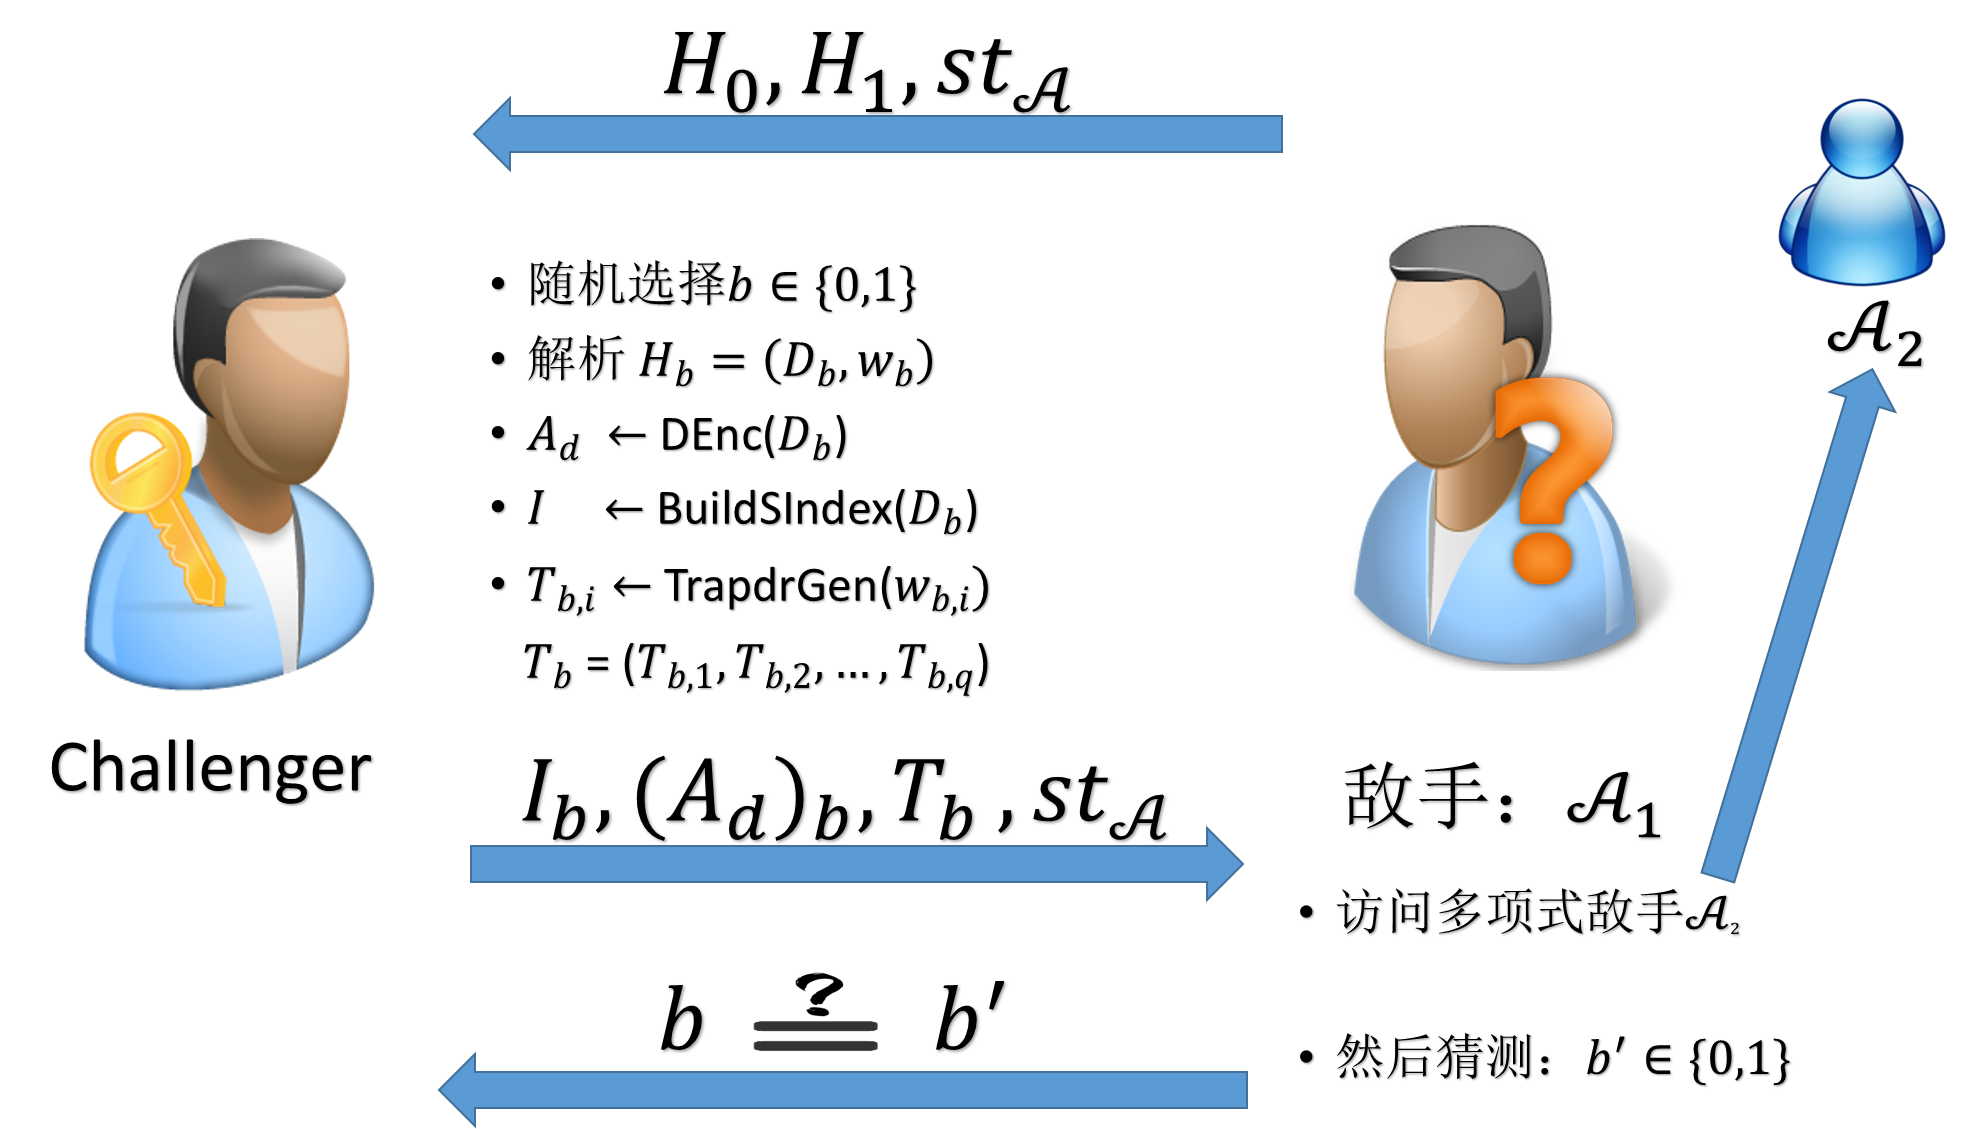
\includegraphics[width=0.9\textwidth,scale=0.8]{chap3/searchpattern_attack_model}
  \bicaption[fig:searchpattern_attack_model]{修改后的方案游戏模型}{修改后的方案游戏模型}{Fig}{New Security Game Model}
\end{figure}

\begin{thm}[$IND\_CKA$ Security]
\label{thm:ind_cka_security_proof}

如果方案中所使用的函数$F$、$P$和$Q$是伪随机函数,$H$和$\phi$是伪随机置换,$\mathcal{G}$是伪随机生成器,并且$SKE$是$PCPA$安全的,则该方案是non-adaptive不可区分安全的。

\begin{proof}
该部分将使用Curtmola方案中提出的Non-adaptive不可区分游戏模型对方案的安全性进行证明。

在游戏过程中,首先敌手$\mathcal{A}_1$发送的历史记录$H_0$和$H_1$,满足$|H_0| = |H_1|$即$|D0| = |D1|$ 且$|w0| = |w1|$, 然后挑战者(Challenger)在过程中随机选择参数b,敌手$\mathcal{A}_1$收到记录后能访问多项式敌手$\mathcal{A}_2$,但在猜测过程中,仅能使用挑战者获得的知识。因而,我们仅仅需要判断敌手对挑战者发起的内容在多项式时间不可区分,从如下几个方面分析:

\begin{itemize}
  \item \textbf{$Setup$:}挑战者$C$随机生成密钥$K$;

  \item \textbf{$DEnc$:}当$C$收到敌手$\mathcal{A}_1$发送过来的历史信息$H_0$和$H_1$后,随机选择参数$b$,然后解析历史$H_b$并对文档加密生成$(A_d)_b$,并送至敌手;

  \item \textbf{$BuildSIndex$:}同样地挑战者收到挑战的历史记录后,对$D_b$建立安全索引$I_b$;

  \item \textbf{$TrapdrGen$:}  挑战者$C$对$w_b$中每个单词,计算对应的陷门,并送至敌手$\mathcal{A}_1$。
\end{itemize}

在上述所有过程中,挑战者仅仅使用了安全的伪随机过程和$PCPA$安全的对称加密方案SKE,它们仅都在多项式时间内以不大于1/2+$negl(k)$的概率进行区分。因此,当敌手收到$C$发送过来的信息后,即使敌手$\mathcal{A}_1$ 有能力访问算法$\mathcal{A}_2$,仍不能猜中$b' = b$ 的概率大于1/2。所以,我们的方案是non-adaptive不可区分安全的。

另外,我们的方案在搜索时,一个单词对应有$q$个不同的单词陷门,并且同一个单词陷门访问文件块时有$p$ 种情况和相同文档中一块指向下一对应块的连接是随意的(每个文件块包含$p$份),故敌手能推断出搜索模式的概率仅为$q*2^p$。因不同的单词同样含有相同的文档,故能推断出搜索模式的概率小于$q*2^p$。

\end{proof}
\end{thm}



%%%%%%%%%%%%%%%%%%%%%%%%%%%%%%%%%%%%%%%%%%%%%%%%%%%%%%%%
%%
%%    性能分析
%%
%%%%%%%%%%%%%%%%%%%%%%%%%%%%%%%%%%%%%%%%%%%%%%%%%%%%%%%%
\section{性能分析}
\label{sec:searchpattern_capability}
到此,我们已经完成了整个方案的功能,不仅能避免size pattern的泄漏,以概率泄漏搜索模式和访问模式,同时也通过严格的分析证明了我们方案在我们的模型下是安全的。下面我们从三个方面对我们方案的性能进行分析 --- 存储开销、计算开销和传输开销。

\subsection{存储开销}
\label{sec:searchpattern_capability_storage}

为了减少更多的信息泄漏,方案不得不引入额外的存储开销。下面我们从两个方面分析方案的存储性能:
\begin{enumerate}
  \item \textbf{索引结构:}在方案中,我们使用查询表$T$和数组$A$来存储安全索引。在建立查询表过程\ref{alg:BuildLookup}中,对每个单词存储p份,因而$T$的存储空间大小为:$W(D) * q * |T[i]|$ ($T[i]$ --- 表示查询表中每个结点所需要的大小)。在文档ID数组的建立过程
      \ref{alg:BuildArray} 中,对每个单词$w$,存储被文档包含的ID数组,并且通过填充使每个ID数组大小保持相等,因而数组$A$的存储空间大小至少为:$W(D) * ID(w_i) * A[i]$($w_i \in W(D)$,$A[i]$ --- 表示数组每个结点所占用空间)。

  \item \textbf{文档结构:}在加密文档过程\ref{alg:DEnc}中,首先对每个文档进行填充使大小为文档的最大大小并分块,并对每块复制$p$份,因而文档块数组$A_d$的大小至少是:$|D_i| * p$。

\end{enumerate}


\subsection{计算开销}
\label{sec:searchpattern_capability_computing}

我们从客户加密、陷门生成和服务端查询三个方面对方案的计算性能进行分析。
\begin{enumerate}
  \item \textbf{加密文档:}在数据所有者外包数据之前,首先对文档进行加密,涉及到建立索引和文档加密。在文档加密阶段,客户的计算开销花费在对数据分块是调用函数SKE.Enc进行简单的加密处理,计算时间为:$|D| * m * T(SKE.Enc)$($T(SKE.Enc)$ --- 表示算法SKE.Enc加密所使用的时间)。索引建立的时间主要包括生成斯密斯正交基和建立安全索引,其计算时间开销为:$T(s) * |W(D)| + |W(D)| * q * ID(w_i)$ ($w_i \in W(D)$, $T(s)$ --- 表示生成正交基所花费的时间)。

  \item \textbf{陷门计算:}在陷门生成算法计算过程\ref{alg:TrapdrGen} 中,首先需要获得待查寻单词$w$的一个正交基(计算过程与算法BuildLookup相同),然后基于该向量构建该向量的法平面,因而客户端的计算开销为:$T(s) + T(M)$,这里$T(s)$和$T(M$分别表示生成单词$w$的基和该基向量的法平面所需要的时间。

  \item \textbf{文档查询:}在算法Query\ref{alg:Query}过程中,服务器需要分别遍历安全索引和文档块数组,这里假设在数据$A$和$A_d$中单步的计算开销为$O(1)$,则总时间计算开销为:$|ID(w_i)| * m$ ($w_i \in W(D)$,$m$ --- 表示每个单词所查找到的所有文件块总大小)。
\end{enumerate}

\subsection{传输开销}
\label{sec:searchpattern_capability_transmission}

传输开销主要发生在客户与服务器之间的通讯阶段,因而,我们可以从上传文档、发送搜索陷门和返回检索结果这三个方面来分析网络的负荷。

\begin{enumerate}
  \item \textbf{文档上传:}在文档上传阶段,客户上传至服务端的信息包括索引结构$I$ 和加密文档结构,因而该次通讯开销的总大小为:$|A| + |T| + |A_d|$。

  \item \textbf{搜索陷门提交:}在该阶段,用户上传的陷门内容仅仅包括待查单词的几个伪随机函数,因而我们可以简单地将通讯时间看作为$O(1)$,与其它方案的开销保持在同一个级别。

  \item \textbf{检索结果返回:}在服务器返回符合搜索条件的结果至客户过程中,传输的信息量记为查询过程所得的结果大小,因而传输开销的大小同样为:$ID(w_i)| * m \ (m \approx |D_i|)$ 。由于在每次用户查询过程中,都需要计算和传输该数据,因而应该尽可能地减小其大小。

\end{enumerate}





%%\section{基于可信第三方的方案}
%%\label{sec:searchpattern_trusted_third_party}
%%
%%这里,简单介绍一个如何使用可信第三方来真正确保trace信息的泄漏。使用可信第三方的系统模型如图
%%\ref{fig:searchpattern_trusted_third_party}所示:
%%\begin{figure}[!htp]
%%  \centering
%%  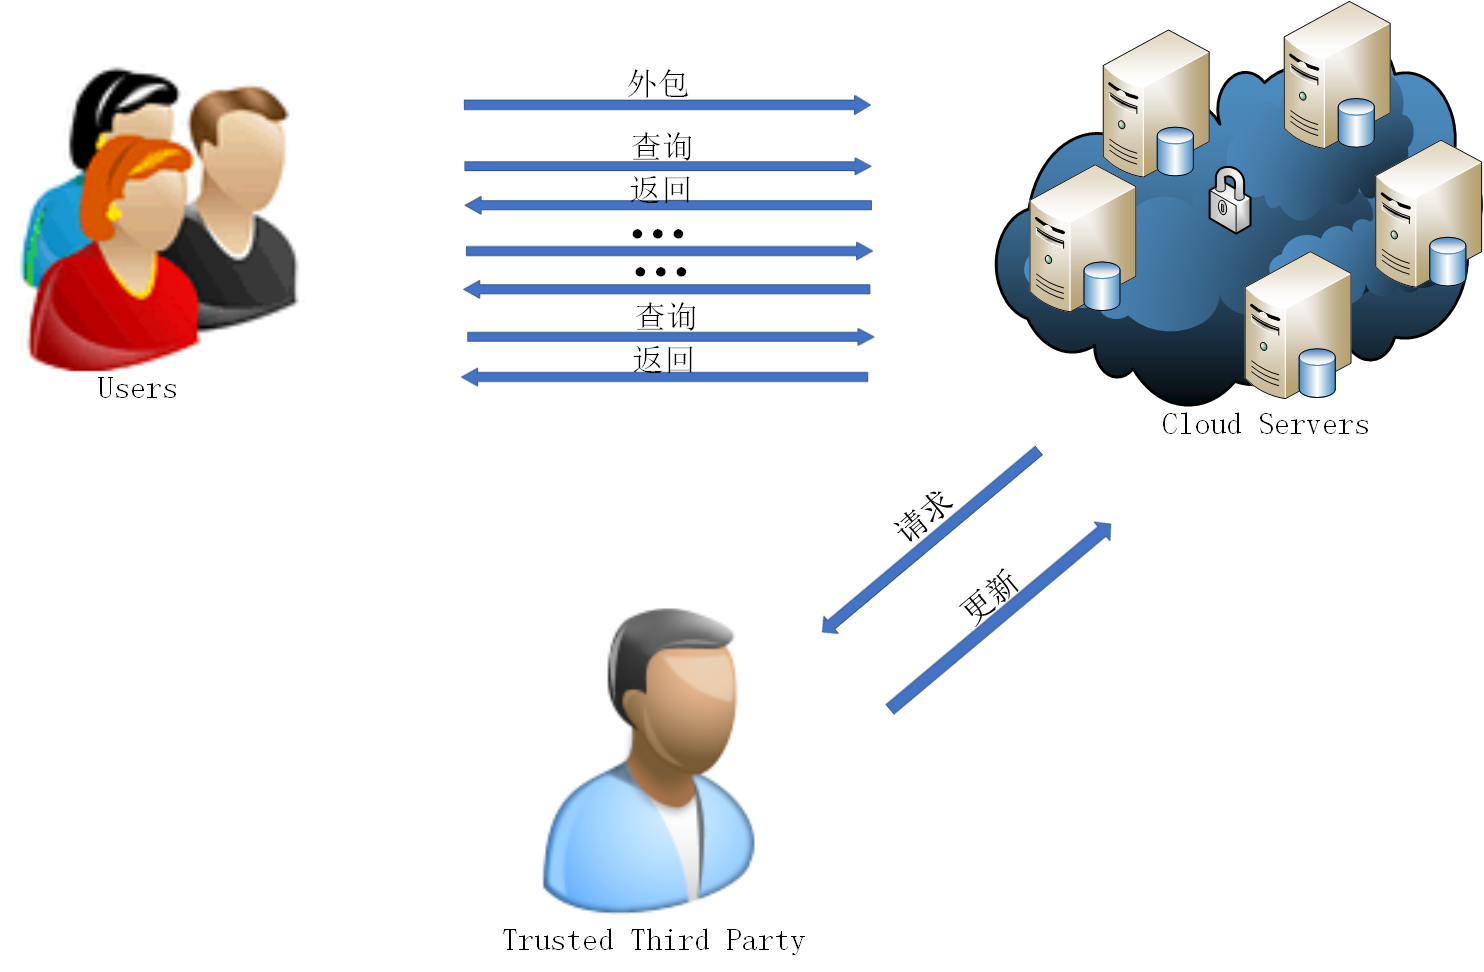
\includegraphics[width=0.9\textwidth,scale=0.8]{chap3/searchpattern_trusted_third_party}
%%  \bicaption[fig:searchpattern_trusted_third_party]{基于可信三方的系统模型}{基于可信三方的系统模型} {Fig}{The System Model Based on Trusted Third Party}
%%\end{figure}
%%
%%在该模型中,我们设计的方案与上述可搜索加密算法相比,主要在以下几个过程上有所不同:
%%\begin{itemize}
%%  \item \textbf{安全索引的存储:}由可信第三方存放安全索引;
%%
%%  \item \textbf{陷门生成:}授权用户提交陷门至可信第三方;
%%
%%  \item \textbf{结果查找:}可信第三方将所需的文档信息发给给服务器,服务器之间返回结果给请求者。
%%\end{itemize}

%%\section{基于三方方案的构造}
%%\label{sec:searchpattern_how_build}

%%\section{应用}
%%\label{sec:searchpattern_application}



%%==================================================
%% chapter03.tex for SJTU Master Thesis
%% Encoding: UTF-8
%%==================================================

%%%%%%%%%%%%%%%%%%%%%%%%%%%%%%%%%%%%%%%%%%%%%%%%%%%%%
%%
%%   同义词对称可搜索加密
%%
%%%%%%%%%%%%%%%%%%%%%%%%%%%%%%%%%%%%%%%%%%%%%%%%%%%%%
\chapter{同义词对称可搜索加密}
\label{chap:synonym}

到目前为止,对称可搜索加密技术已得到广泛的研究,各种复杂的条件搜索加密技术也被深入的研究并取得了实质性的成果。然而在复杂的多变的云计算环境下,我们需要研究的知识点范畴广和面对的用户群里基数大。为此,我们不得不进一步挖掘出一些尚未提出并具有实际意义的问题。在前人的工作指导下,本文解决了相似搜索的另一个场景 --- 同义词搜索。

在本章,我们提出了一个支持同义词搜索并具有强安全性的对称可搜索加密方案。为此,我们首先定义了方案的系统模型和攻击模型;然后定义其算法框架;针对方案框架的各个算法,逐个给出它们的详细实现细节;最后我们对该方案进行了严格的安全性证明和性能分析。



%%%%%%%%%%%%%%%%%%%%%%%%%%%%%%%%%%%%%%%%%%%%%%%%%%%%%
%%
%%   方案模型
%%
%%%%%%%%%%%%%%%%%%%%%%%%%%%%%%%%%%%%%%%%%%%%%%%%%%%%%
\section{方案模型}
\label{sec:synonym_model}

在该小节,我们从已有的方案中抽象出将研究的问题;然后针对我们的问题,提出了相应的系统模型和有效的攻击模型;为了实现方案的详细细节,我们引入一些相关的符号及其描述,同时定义了方案的信息泄漏;最后,我们简略地描述了方案的基本框架。

%%在该小节,我们从已有的方案中抽象出将研究的问题;然后针对我们的问题,提出了相应的系统模型;并针对该系统模型,我们提出了有效的攻击模型;为了实现方案的详细细节,我们引入一些相关的符号及其描述,同时定义了我们方案中的信息泄漏;最后,我们简略地描述了我们方案的基本框架。

\subsection{问题提出}
\label{sec:synonym_problem}

%生活在网络高速发达的时代,数据的产量以指数的量级增长,大数据的时代已到来,为解决人们难以应付的难题,可搜索加密方案被提出并解决了大数据中存储和计算的问题。然而,在网络竞争时代,

可搜索加密技术解决了外包数据的安全和高效搜索的难题。然而,在互联网快速发展的时代下,人们在工作中的强度日益增加,致使人们的记忆力也随着超载工作量的过度消耗而呈现下降趋势。由于人们记忆能力的周期的缩短和人员频繁的变换,使得一段时间之后,他们对之前使用过的文档及其内容的记忆已模糊不清甚至完全遗忘。此情景的一个典型的示例如图\ref{fig:synonym_problem}所示。首先,使用云计算平台服务的数据所有者将文档外包至不可信的云端;一段时间后,数据所有者想要查找包含“文件”含义的关键字的文档时,其可能因忘记不知道文档中到底包含“paper” 还是“document”?为此,用户不得不逐个尝试所有具有该含义的单词,直至找到所需的答案为止。在按计算收费的时代,这显然是不合理的,同时也增加了网络带宽和用户的响应时间。%为解决此场景引出的问题,该章提出了一个新的解决方案 --- 同义词对称可搜索加密技术。
\begin{figure}[!htp]
 \centering
 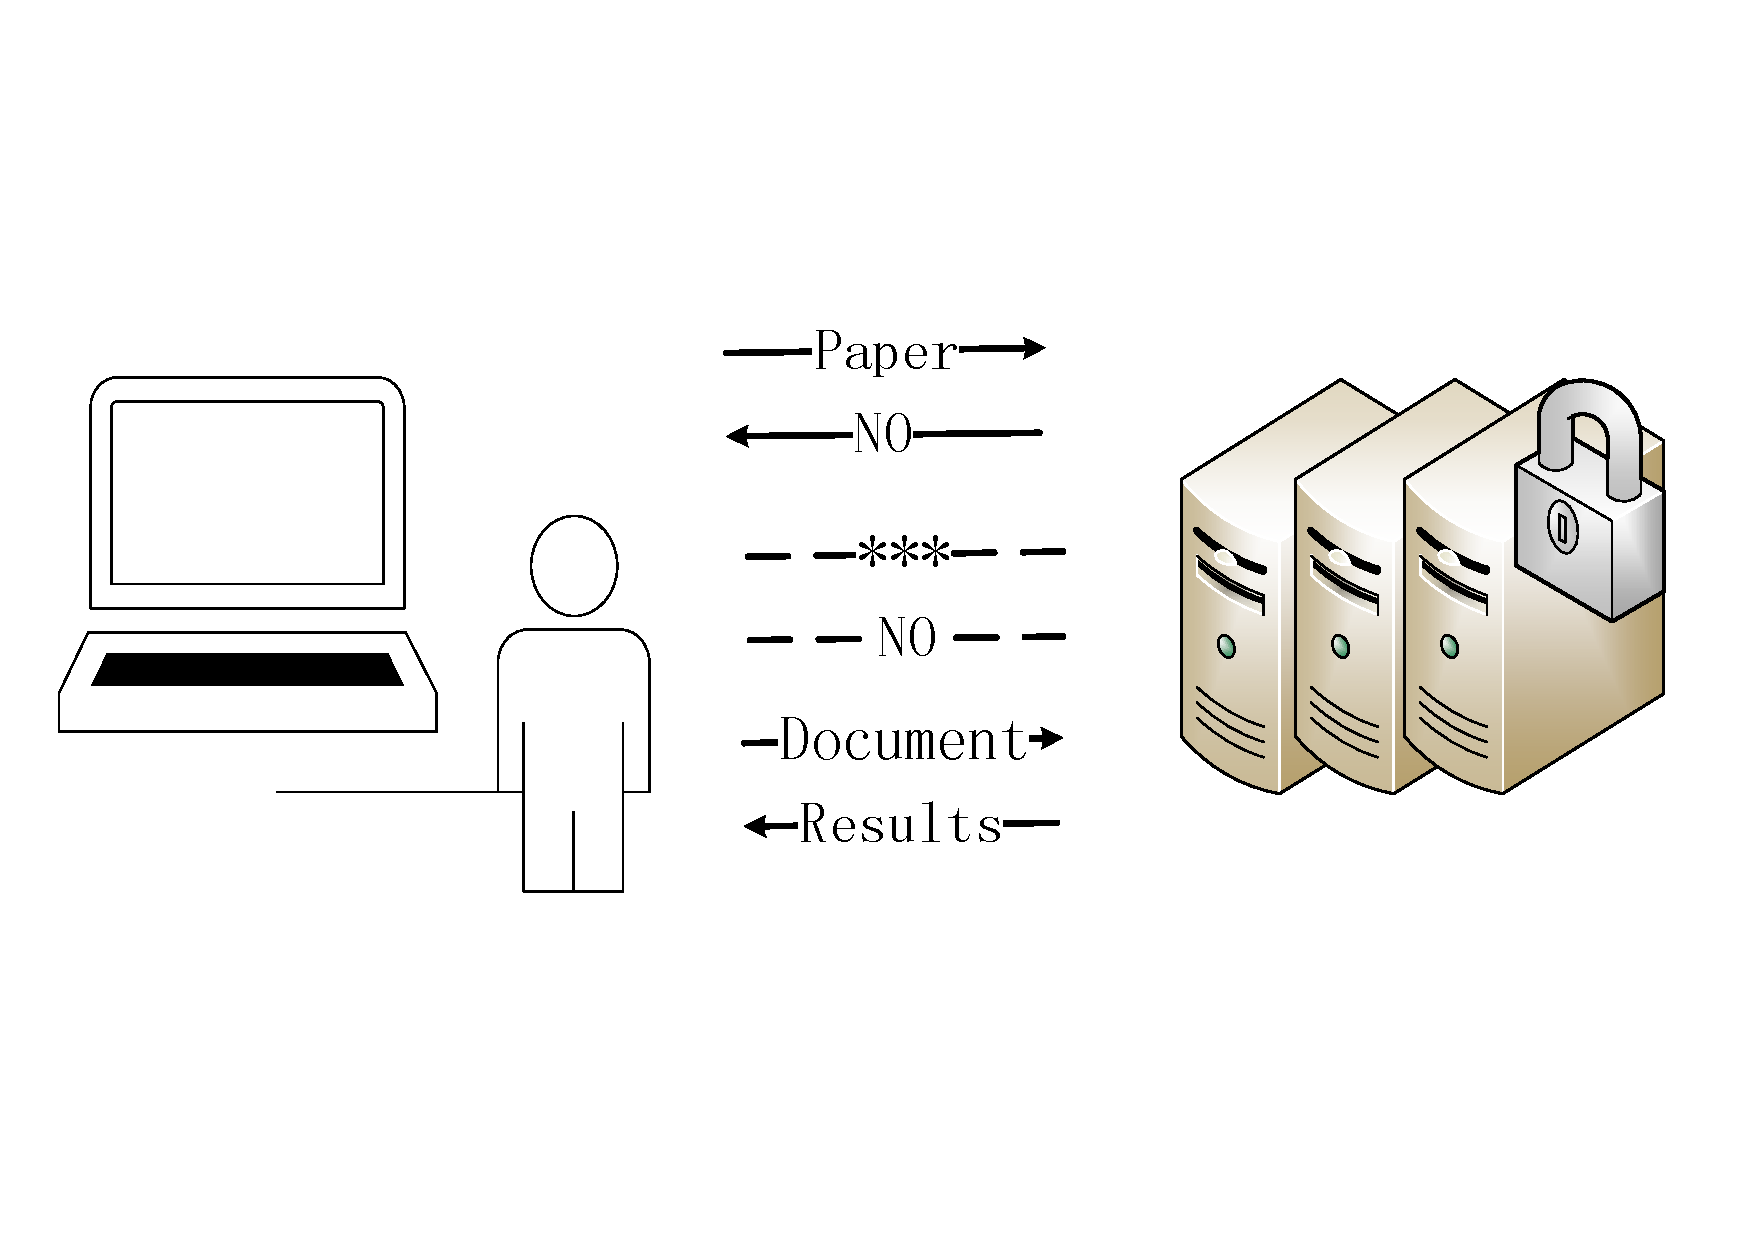
\includegraphics[angle=0,origin=br,width=15cm]{chap4/problem.pdf}
 \bicaption[fig:synonym_problem]{同义词可搜索加密方案的示例}{同义词可搜索加密方案的示例}{Fig}{An Example of the Synonym Search}
\end{figure}



\subsection{系统模型}
\label{sec:synonym_model_system_model}

在我们的方案中,支持同义词搜索的系统模型(如下图\ref{fig:synonym_system_model}所示)包括三部分 --- 数据所有者(Owner),授权用户(Users)和云服务提供商(Provider)。这三部分在系统中分别承担不同的角色。数据拥有者是数据的源头和拥有系统的抉择权,授权用户是系统中最频繁的访问者,而云服务提供商是系统的服务提供者和数据的响应者。
\begin{figure}[!htp]
 \centering
 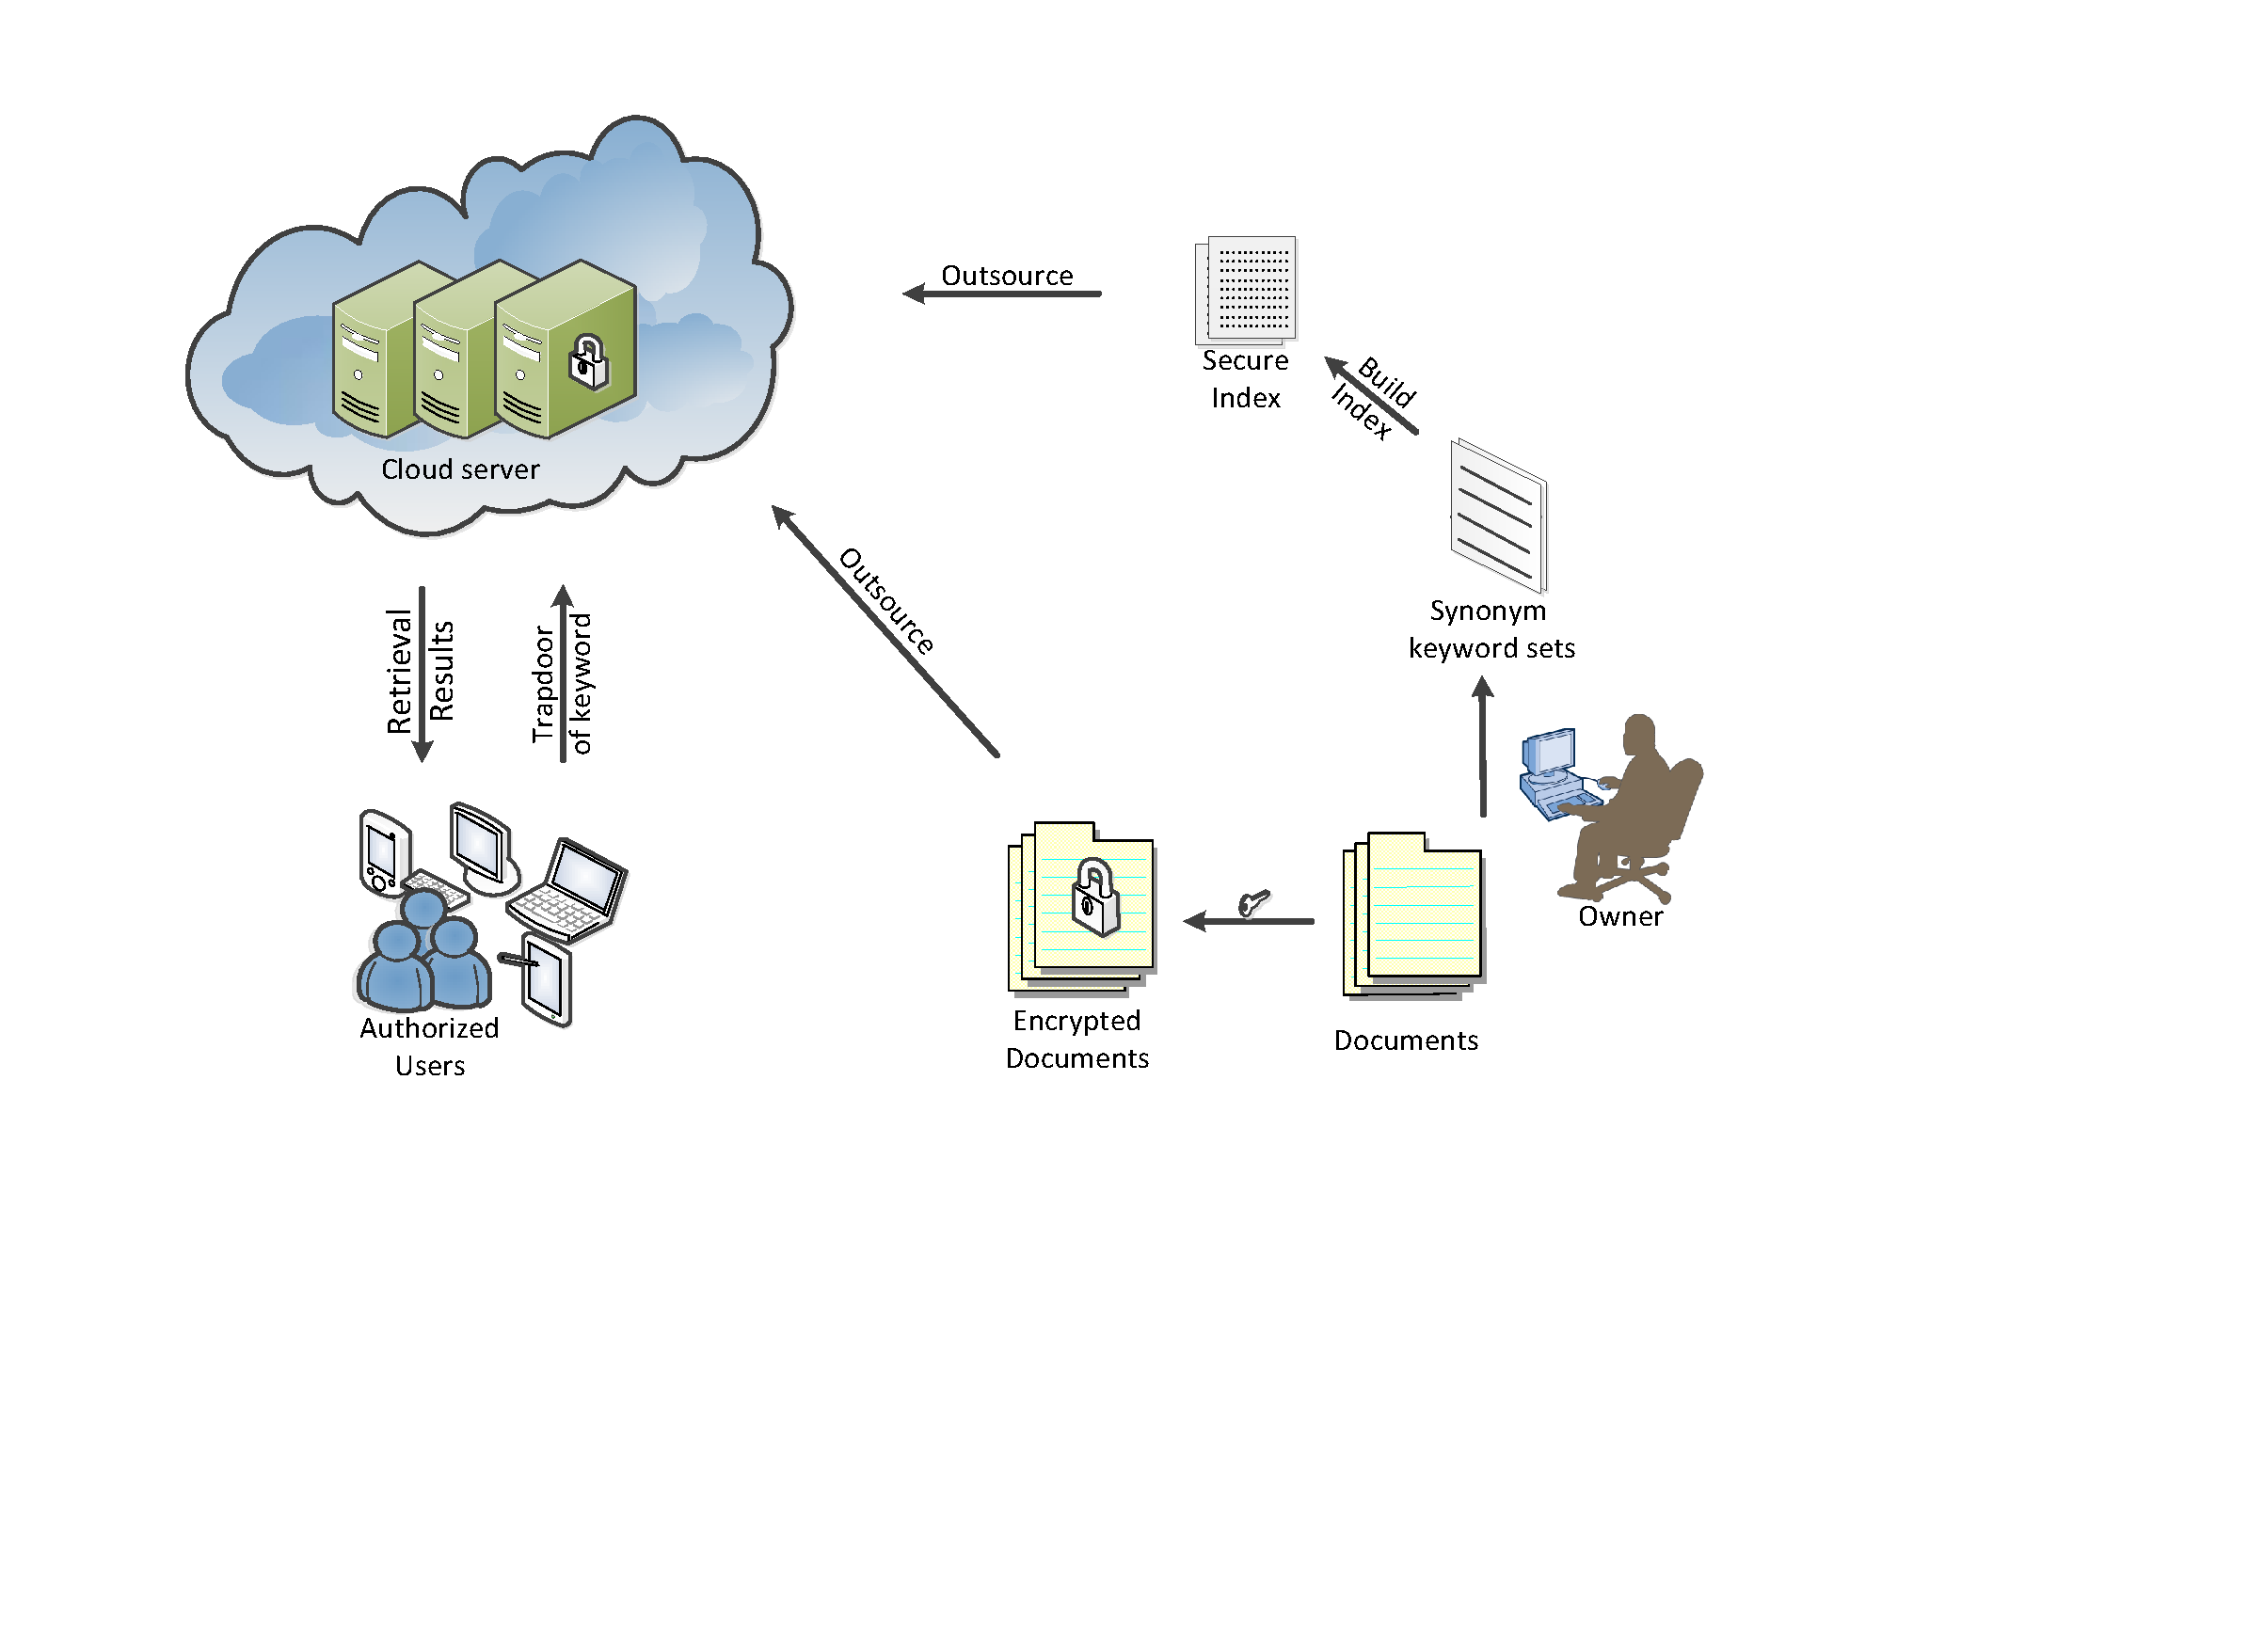
\includegraphics[angle=0,origin=br,width=15cm]{chap4/system_model.pdf}
 \bicaption[fig:synonym_system_model]{同义词可搜索加密系统模型}{同义词可搜索加密系统模型}{Fig}{The System Model of Synonym Search}
\end{figure}


\begin{enumerate}
  \item
  \textbf{数据所有者:} 数据所有者是系统的主体,拥有系统中最核心的部分---数据。数据拥有者往往由一个公司、组织或团体组成。同时,数据拥有者需要考虑系统的性能、功能和其它各种因素。一般情况下,当数据拥有者想利用外包端的便利服务时,需先购买云服务,将所有的数据首先加密,然后存储到云服务提供商。



  \item
  \textbf{用户:} 用户是系统的使用者,往往是系统中最大的人群(包括数据所有者)。用户往往不考虑系统的任何细节,只希望利用系统提供的便利和安全性。通常情况下,如果一个用户想要使用系统的查询功能,首先他必须征求数据拥有者的允许---即获得请求数据的安全密钥,成为合法的请求者;然后利用安全密钥生成单词陷门,并提交任务给云端;最后,在收到响应结果后,对其进行解密,获得所需的文档。在我们系统中,返回的结果包括所有包括该单词和与它有相同含义的单词的文档。



  \item
  \textbf{云服务提供商:} 云服务提供商是系统的客体 --- 系统功能服务者,用于对外包数据进行存储和计算,是系统必不可少的一部分。通常情况下,首先接收数据所有者提交至云端的加密数据和索引,并提供对数据的计算和备份工作。当收到用户提交的查询请求时,然后利用强大的计算能力对数据进行查询操作,并将匹配的结果返回给请求者,若不存在则返回空。
\end{enumerate}

在同义词可搜索加密方案中,云服务提供商返回的结果集包括两部分:(1)包含待查单词的文档;(2)包含与待查单词有相同含义的单词的文档。即返回的信息可描述为:$ED = \{ ED_i | w \in D_i, w \in S_w \}$。并且证明我们方案具有non-adaptive安全。

%%在我们的系统中,若云服务提供商是安全并且诚实的,因而我们系统中外包的数据是安全的 --- 数据使用安全函数加密。但是,在通常情况下,云服务提供商虽然表面上遵照系统协定提供安全的云服务,而本身又是“honest-but-curious” ---- 因对数据好奇而暗地里偷偷地分析用户查询的数据,然后根据其他知识(例如单词的统计信息)来推断用户所搜索的真实单词,这足以说明我们方案仍存在一定的信息泄漏。为此,我们必须精确量化出系统信息泄漏的大小,通常将云服务器视为具有最强计算能力的敌手,能分析出的数据即为系统的信息泄漏量。

\subsection{攻击模型}
\label{sec:synonym_model_attack_model}

在我们的系统中,若云服务提供商是安全并且诚实的,因而我们系统中外包的数据是安全的 --- 仅使用了安全的伪随机函数和$SKE.Enc$对数据加密。不幸的是,通常来说云服务提供商是“honest-but-curious” --- 即遵照系统所定义的协定进行操作,同时因对数据好奇而暗地里偷偷地分析用户查询的数据,然后根据一些其他知识(例如单词的统计信息)来推断用户所搜索的真实单词,这足以说明以上方案仍存在一定的信息泄漏。为此,我们必须精确地量化出系统信息泄漏的大小,通常将云服务器视为具有最强计算能力的敌手,能分析出的数据即为系统的信息泄漏量。为了衡量我们所定义信息泄漏的正确性,引入了安全的分析模型,以证明方案除了泄漏必不可少的信息之外,不泄露其他任何的信息。为了证明方案具备Non-adaptive安全,假设$\mathcal{A}$ 是多项式的敌手,$\mathcal{S}$是模拟者,方案的攻击模型如下:


%%在我们的方案中,如果云服务提供商是绝对安全并且诚实的,则我们系统中外包的数据必是安全的 --- 仅使用伪随机函数和$SKE.Enc$对数据加密。不幸的是,通常来说云服务提供商是“honest-but-curious” --- 即遵照系统所定义的协定进行操作,同时因对数据好奇而暗地里偷偷地分析用户查询的数据,然后根据一些其他知识(例如统计信息)来推断我们查询的内容,这致使我们的数据仍处理一定的风险。为此,我们必须清楚地了解到云服务到底能分析出多少信息。为了分析我们系统泄漏信息量的大小,我们通常将云服务作为敌手,在他们有最强的计算能力的亲情况下,分析出的数据即为我们系统的信息泄漏量。为了衡量我们所定义信息泄漏的正确性,引入了安全的分析模型,以证明方案除了泄漏我们所定义的信息之外,不泄露其他任何的信息。这里我们定义我们方案具有Non-adaptive安全,假设$\mathcal{A}$是多项式的敌手,$\mathcal{S}$是模拟者,方案的攻击模型如下:

\begin{center}
\begin{tabular}{ l l }
    $\textbf{Real}_{SSE,\mathcal{A}}(k)$  &  $\textbf{Sim}_{SSE,\mathcal{A},\mathcal{S}}$    \\
    \quad $K \leftarrow SSGen(1^k)$ & \quad $(H,st_\mathcal{A}) \leftarrow \mathcal{A}(1^k)$ \\
    \quad $(st_\mathcal{A},H) \leftarrow \mathcal{A}(1^k)$ &\quad $V^* \leftarrow S(\tau (H))$\\
    \quad parse $H$ as $(D,w)$          &   \quad output $V^*$ and $st_\mathcal{A}$     \\
    \quad $(SI,KED) \leftarrow SSEnc(D,K,SD)$            &   \\
    \quad for $1 \leq i \leq q $                 &   \\
    \quad \quad $T_{w_i} \leftarrow SSTrapdoor(w_i,K)$    &   \\
    \quad let $T_w = (T_{w_i}, ..., T_{w_q})$              &    \\
    \quad output $V = (SI,KED,T_w)$ and $st_\mathcal{A}$    &
\end{tabular}
\end{center}



\subsection{相关定义}
\label{sec:synonym_model_related_definition}

%%在这里,我们定义了一些与方案相关的符号,如下(Note:X --- 代表是一个数据结构,包括链表、数组或文档等等;n --- 任意大小):
\begin{itemize}
%  \item
%  $|X|$ --- 结构X的长度,即X中单词的个数。

  \item
  $ [n] $ --- 表示$n$个元素的集合,等价于 $\{ 1, ..., n \}$。

  %\item
%  {$ max(|S|) $} --- 如果S是集合,则它代表集合S的元素数目|S|;若S是集合的集合,则它表示集合S 中所有元素的最大数目,即$max\{|S_i|$ | $S_i \in S\}$。

  \item
  $D$ --- 所有待外包的文档的集合,$n$个文档的集合 $D$ = ($ D_1, D_2, ..., D_n $)。

  \item
  $ID(D)$ --- 文档$D$的ID信息,可以用数字表示也哈希值来唯一表示。

  \item
  $ED$ --- 加密文档的结合,$n$个密文文档的集合 $ED$ = ($ ED_1, ED_2, ..., ED_n $)。

  \item
  $KED$ --- 所有加密文档键值对$<$ $ID(D_i)$, $ED_i$ $>$的集合($ ED_i \in ED $)。

  \item
  $W(X)$ --- 结构$X$中所有不同单词所组成的集合,表示为:$W(X) = (w_1, w_2, ..., w_{|W(X)|})$。

  \item
  $D_w,SD_w$ --- $D_w$是仅包括单词$w$的所有文档的集合;$SD_w$是包括单词$w$和其同义词的文档的集合。

  \item
  {$SD$}--- 同义词字典的集合,它必须包含集合$W(D)$中的所有单词。根据所定义环境的不同,集合中元素也不相同。$m$个元素的集合$SD$,表示为:$SD$ = ($ w_1, ..., w_m $)。

  \item
  $ S_w $ --- 单词$w$的所有同义词的集合,描述为:$ S_w = (w_1, w_2, ..., w_{|S_w|}) $。

   \item
  $ SID_w $ --- 包含单词$w$的文档的ID集合,定义$ SID_w = \{ID(D_i) $ $|$ $ w \in D_i\}$, $SID$ = $\{SID_w$ | $w_i \in W(D) \} $。

  \item
  ${SI}$ --- 安全索引结构,由数据拥有者生成,并存储在云服务端。在我们系统中使用数组和查询表来维护。

  \item
  $ T_w $ --- 单词$w$的陷门信息。它使用伪随机函数生成,用于在搜索过程中作文查询口令。

  \item
  $ ESD_w $ --- 用户在查询后,由服务器返回的加密的文件集合。


%%  \item
%%  $F(K,*)$ --- 如果我们定义函数$F$为: $ \{0, 1\}^k * \{0,1\}^n \rightarrow \{0, 1\}^m $,且在多项式时间内,函数F是可计算的和对于一个具有多项式访问oracle的敌手A,有: $|Pr[A^{f_k(.)} = 1 : K \leftarrow \{0,1\}] - Pr[A^{g(.)} = 1: g \leftarrow Func[n,m]]| \leq negl(k)$,则称函数F 为伪随机函数(PRF),若函数F是双射,我们称它为伪随机置换(PRP)。
%%
%%  \item
%%  ${ SKE = (Gen, Enc, Dec) }$ --- 定义SKE是私钥加密方案。在标准SKE中,Gen是伪随机函数, 用于生成密钥K;Enc用于将给定的值进行加密;而Dec则用于解密。对于任意给定的两个密文,我们不能判断是否被同一个密钥加密。
\end{itemize}

%
% Definition: Synonym Function
%
\textbf{同义词函数(Synonym Function)} 对于任意给定的两个单词$w_1$和$w_2$,定义:
\begin{equation}
SF(w_1, w_2) =
\begin{cases}
1 & \text{ if ${w_1}$ and ${w_2}$ is synonym}
\\
0 & \text{ otherwise }
\end{cases}
\end{equation}
在上述公式中,如果输出结果为1,则称单词$w_1$和$w_2$相似,称函数$SF$为相似判断函数(简称相似函数)。

%
% Synonym dictionary
%
%%\textbf{同义词集合(Synonym Sets)} 对于给定的单词w ($ w \in SW$),定义同义词集合为:$ SWS = \{S_{w_i}$ $|$ $ w_i\in S_w \} $。在我们的系统中对于$SW$,我们取英文字典中的所有单词,其原因是:如仅包含单词W(D),若我们查询单词“document”时,而文中不包括“document”仅包含“paper”,则输入则无效,这将大大降低方案的可用性。在实际中,我们可以根据环境的不同来定义SW,甚至我们能动态地根据环境信息搜索建立SW集合。



%
% Definition: Information Leakage
%
\textbf{信息泄漏} 在我们的方案中,我们主要分析我们所定义场景下的信息泄漏情况,我们定义该方案信息泄漏包括文档大小、访问模式和搜索模式。这里我们不考虑文档大小,仅从搜索模式和访问模式信息泄露进行分析。

\textbf{查询历史:} 具体定义请参见\ref{defn:attack_history}。

\textbf{搜索模式:} 给定文档集$D$和$q$次查询历史$H$,定义搜索模式如下:\\
 $\sigma(H) = \begin{bmatrix}
 &x_{1,1}  &x_{1,2}  &...  &x_{1,q} \\
 &x_{2,1}  &x_{2,2}  &...  &x_{2,q} \\
 & . & .   &...      &. \\
 & . & .   &...      &. \\
 & . & .   &...      &. \\
 &x_{q,1}  &x_{q,2}  &...  &x_{q,q} \\
\end{bmatrix}$,其中$x_{i,j}$可能取值0、1、2。若$x_{i,j}$为0 --- 表示$w_i$和$w_j$为不相等且没有相同的同义词集合$S_w$;取值1 --- 表示$w_i$和$w_j$不相等但是有相同的同义字集合;取值2 --- 表示$w_i$ 和$w_j$ 为相同的单词。

\textbf{访问模式:} 对于给定文档集$D$和$q$次查询历史$H$,定义访问模式 $\partial(H) = (SD(w_1), SD(w_2), ... SD(_q))$,$SD(w_i)$ = $\{D(w_j)$ | $w_j \in S_w$ $\}$。

\textbf{Trace:} 对于给定大小为$n$的文档集$D$和$q$次查询历史$H$,定义其Trace信息为元组:$\tau(H) = (|D_1|, ..., |D_n|, \sigma(H), \partial(H))$。


\subsection{方案描述}
\label{sec:synonym_model_scheme_description}
%在我们的方案中,主要解决对称可搜索加密环境下同义词搜索(SSSE)的场景,即输入单词w,即返回包含单词w 的文档,同时返回包括和单词w有相同函数的文档的问题。下面简单描述我们的方案。\\

下面我们简单地描述我们方案:\\
%
% Definition: Synonym Searchable Encryption
%
\textbf{Synonym Searchable Encryption(SSSE):} 方案包括由5个基本的算法组成,定义:$SSSE$ =($SSKeyGen, SSEnc, SSTrapdoor, SSSearch, SSDec$)。
\begin{description}
  \item[$\{K\} \leftarrow SSKeyGen(1^k)$:]是一个概率密钥生成算法,输入安全参数$k$和输出密钥$K$。
  \item[$\{SI, KED\} \leftarrow SSEnc(D, K)$:]是方案中主要的加密模块,输入参数文档集合$D$和密钥$K$,输出安全索引$SI$和加密文档$KED$。主要包括文档加密函数($SSDEnc$)和安全索引建立函数($SSBuildSI$)。
  \item[$\{T_w\} \leftarrow SSTrapdoor(w, K)$:]是一个确定性的算法(可能是概率算法)。对于一个给定的单词$w$,在密钥$K$下,生成陷门${T_w}$。
  \item[$\{ESD_w\} \leftarrow SSSearch(T_w, SI, KED)$:]是一个确定性算法。输入待查询单词$w$的陷门$T_w$、$SI$ 和$KED$,查询并输出同义词结果集${ESD_w}$。
  \item[$\{PSD_w\} \leftarrow SSDec(ESD_w, K)$:]是一个确定性的算法,用于解密。使用返回的结果集${ESD_w}$和加密密钥$K$,并输出解密的文档${PSD_w}$。
\end{description}


%%%%%%%%%%%%%%%%%%%%%%%%%%%%%%%%%%%%%%%%%%%%%%%%%%%%%
%%
%%   算法框架与方案细节
%%
%%%%%%%%%%%%%%%%%%%%%%%%%%%%%%%%%%%%%%%%%%%%%%%%%%%%%
\section{算法框架及细节}
\label{sec:synonym_scheme}

在描述我们的方案之前,仅仅考虑一个简单的情况 --- $SD$中每个单词仅存在一个含义。基于这样的假设,我们设计了一个支持同义词搜索的解决方案并描述方案中各算法的详细实现流程。然后我们阐述了如何将我们方案应用于一词多义的情形并分析我们方案的优势。在详细描述我们方案之前,我们重新回顾同义词字典和同义词集合的概念。

\textbf{关于$SD$的扩展:} 为了使该方案更具通用性,方案中定义同义词字典$SD$为按字典排序的所有的单词集合。它不仅包括$W(D)$中的所有单词,而且包含与文档中单词有相同含义的所有单词。考虑此情况的原因在于:如果我们外包有单词“Paper”但不包含单词“Document”的文档集合$D$至远程服务器;一段时间后,授权用户键入单词“Document”去查找,由于键入没有命中,服务器不得不返回无效的结果集。此时,用户不得不逐个地尝试所有具有相同含义的单词,找到所要查询的文档未知。这将大大降低方案的灵活性和可通用性。另外,用户通常希望在不同的环境下有不同的同义词集合,通常我们可能根据某领域内用户的查找知识来动态建立同义词字典。例如,在医疗行业,同义词字典的集合与其它领域可能有所不同,我们可以根据客户的要求来建立$SD$。 这样定制的同义词集合将使我们方案的查询性能更好和返回的结果集更有意义。

\textbf{同义词集合的构建:}通常情况下,同义词集合仅仅考虑文档中所有不同单词集合$W(D)$,而忽略了其它单词。在我们构建的方案中,基于同义词字典,建立同义词集合如下:
\begin{enumerate}
  \item
  对每个单词$w \in W(D)$,初始化单词的同义词集合$S_w = \{w\}$;
  \item
  然后对每个单词 $w_i \in \{SD \setminus w\}$,计算$SF(w, w_i)$,如果结果为1,则插入单词$w_i$ 至集合$S_w$,否则跳过它;
  \item
  最后定义文档的同义词集合$SWS = \{S_w | w \in W(D) \}$。
\end{enumerate}



\subsection{\textbf{框架详细描述}}
\label{sec:synonym_scheme_description}

\textbf{同义词对称可搜索加密:} 定义同义词对称可搜索加密方案由五个算法组成即 $PSSSE = (SSKeyGen, SSEnc, SSTrapdoor, SSSearch, SSDec)$。$SSKeyGen$用于生成密钥;$SSEnc$算法由三个子算法($SSInitSets$ --- 用于初始化文档集合,$SSDEnc$ --- 加密文档,$SSBuildSI$ --- 对文档建立安全索引)组成;$SSTrapdoor$ 生成单词的陷门;$SSSearch$通过陷门查找结果集;$SSDec$仅仅是个简单的解密过程。


%%%In the detailed algorithms definition, we will make full use of the functions $F$, $G$, $P$, $\mathcal{H}$, $\mathcal{G}$, where $F$, $G$ and $P$ are pseudo-random function, $\mathcal{H}$ is the pseudo-random permutation, and $\mathcal{G}$ is pseudo-random generator. To the store the secure index, we use search table $A_t$ and array $A_s$ where $A_t$ is search table of keyword trapdoor in secure index, and $A_s$ is array including all nodes of document ID in $SI$. We define: $SIZE(A_t)$ and $SIZE(A_s)$ are the size of padding additional entries, $max(|SID|)$ and $max(|SWS|)$ are respectively the maximum size of any one element in $SID$ and $SWS$, e.g. $max(|SID|) = (|SID_w|$  $|$  $SID_w \in SID$), where $|SID_{w_i}| \leq |SID_w|$ for any $w_i \in W(D), SID_{w_i} \in SID $. A detailed description of our solution is in Figure \ref{fig:core_algorithm} (Note: in this solution, we only consider each keyword as one meaning, and we will introduce how to dispose of the context of multi-meanings of keyword in the subsequent subsection.)

在详细地描述我们的方案之前,这里首先定义一些将被使用的函数和数据结构,如下:
\begin{itemize}
  \item
  函数$F$、$G$和$P$是伪随机函数;

  \item
  $\mathcal{H}$是伪随机置换;

  \item
  $\mathcal{G}$是伪随机生成器;

  \item
  $A_t$是一个足够大的查询表,用于存储到此的陷门内容,通过此可以找到包含文档$ID$的信息。$SIZE(A_t)$ 表示查询表实际所使用的大小,即未填充时所使用的大小;

  \item
  $A_s$是一个足够大的数组,用户存储文档ID的内容,用户检索到加密文档。$SIZE(A_s)$表示存储文档$ID$ 实际所使用的空间大小。
\end{itemize}

PSSSE方案的各个算法具体实现如下:
%\fbox{
%  \parbox{1.0\textwidth} {
  %
  % insert a long text in here....
  %
    \begin{enumerate}
      %
      % 1. SSKeyGen
      %
      \item
      \textbf{$ \{ K \} \leftarrow SSKeyGen(1^{k}): $} \\
       该算法从集合$ {\{0,1\}}^{k} $中随机选取密钥${ K_1, K_2, K_3 }$,并且调用$SKE.Gen$生成${ SK \leftarrow SKE.Gen(1^{k}) }$,输出$K$ = ($K_1$, $K_2$, $K_3$, $SK$)。

      %
      % 2. SSEnc
      %
      \item
      \textbf{$\{ SI, KED \} \leftarrow SSEnc(D, K):$ } \\
      该算法包括三个子算法$(SSInitSets, SSDEnc, SSBuildSI)$。$SSInitSets$用户初始化操作,$SSDEnc$用于加密文档,$SSBuildSI$用于建立安全索引。它们按如下的顺序执行($SD$在前面被建立):

      \begin{enumerate}
      %
      % SSInitSets
      %
      \item
      \textbf{$ (SWS, SID) \leftarrow SSInitSets(D, SD). $}

      \begin{itemize}
        \item ${ W(D) \leftarrow D }$,遍历文档集$D$,提取出所有不同的单词组成集合:$W(D) = \{w_1, ..., w_{|W(D)|} \}$。

        \item 对每一个单词$ w \in W(D) $,浏览文档$D$构建包含单词$w$的文档的ID集合:$SID_w = \{ID(D_i)$ $|$ $w \in D_i \})$,定义: $SID = \{ SID_{w}$ $|$ $w \in W(D) \}$, 并且确保每个集合的大小与最大集合大小相等。若小于最大集合则使用随机生成的唯一的字符串填充。

        \item 对每个单词$w \in W(D)$,按照上述同义词集合构建过程构建文档的同义词集合。如何集合大小不相等,则通过填入随机的值使得每个集合的大小相等,生成新的集合$SWS$。

      \end{itemize}

      %
      % SSDEnc
      %
      \item
      $ (KED) \leftarrow SSDEnc(SK, D). $ \\
      对每个文档$D_i \in D$,加密生成$ED_i \leftarrow SKE.Enc(SK, D_i)$。然后对每个$ED_i$,设置:$KED_i = <ID(D_i), ED_i>$,并定义$KED = \{ KED_i | i \in [|D|]\}$。

      %
      % SSBuildSI
      %
      \item
      ${ (SI) \leftarrow SSBuildSI(K, SWS, SID). }$ \\
      该算法用于建立方案的核心检索结构 --- 安全索引$SI$,加速查找过程。详细实现细节,请参考算法 \ref{alg:SSBuildSI}。
      % \ref{alg:SSBuildSI}
      \end{enumerate}
      最后,将安全索引$SI$和加密文档内容$KED$外包到远程服务器。


      %
      % 3. SSTrapdoor
      %
      \item
      \textbf{ $ \{ T_w \} \leftarrow SSTrapdoor(w, K): $ }\\
      授权用户使用陷门生成函数输出单词$w$的陷门内容如下:$ T_w =$ $($ $F_{K_1}(w)$, $G_{K_2}(w)$, $P_{K_3}(w)$ $)$,并将请求送至服务器。


      %
      % 4. SSSearch
      %
      \item
      \textbf{$ \{ ESD_w \} \leftarrow SSSearch(T_w, SI, ED): $} \\
      一旦服务器收到远程请求者的陷门,便开始查找安全索引和加密文档,并返回匹配的答案给请求者。具体的实现过程在算法\ref{alg:SSSearchESR}中描述。


      %
      % 5. SSDec
      %
      \item
      \textbf{${ \{PSD_w\} \leftarrow SSDec(SK, ESD_w): }$} \\
      该算法仅涉及到简单的解密过程,最终得到用户需要的解密文档:$PSD_w$ = $\{ SKE.Dec_{SK}(ED_i)  $ $|$ $ ED_i \in ESD_w \} $。

    \end{enumerate}
%  }
% }

%%%%%%%%%%%%%%%%%%%%%%%%%%%%%%%%%%%%%%%%%
%%%
%%%  算法描述
%%%
%%%%%%%%%%%%%%%%%%%%%%%%%%%%%%%%%%%%%%%%%
\subsection{\textbf{算法描述}}
\label{sec:synonym_sheme_algorithm}

\textbf{安全索引建立算法(SSBuildSI):}是一个确定性的算法,在数据被外包之前,由数据拥有者建立。当数据所有者想要使用外包服务时,首先他必须对外包的数据建立索引,并将其存储到数组$A_s$和查询表$A_t$中,同时维持索引之间的联系以及文档$ID$与密文文档的联系。算法\ref{alg:SSBuildSI}实现如下:
%%%%%%%%%%%%%%%%%%%%%%%%%%%%%%%%%%%%%%%%%%%%%%%%%%%%%%%%%%%%%%%%
%%%%%
%%%%%% BEGIN algorithm 1
%%%%%
%%%%% Usage about Reference of Algorithm
%%%%%  Eg: \ref{algorithmLableName}
%%%%%
%%%%%%%%%%%%%%%%%%%%%%%%%%%%%%%%%%%%%%%%%%%%%%%%%%%%%%%%%%%%%%%%
%%%%%
%%%%% Begin algorithms
%%%%%
%%%%\begin{algorithm}[!htb]
%%%%
%%%%%
%%%%% The title of algorithm
%%%%\caption{ $SSBuildSI(K,SD,SWS,SID)$ }
%%%%
%%%%% algorithm label to be referred in the text
%%%%\label{alg:SSBuildSI}
%%%%
%%%%
%%%%\begin{algorithmic} [1]
%%%%
%%%%\REQUIRE ~~\\
%%%%
%%%%  \textbf{${K}$ :}   加密密钥    \\
%%%%  \textbf{${SD}$ :}  同义词字典  \\
%%%%  \textbf{${SWS}$ :} 同义词集合  \\
%%%%  \textbf{${SID}$ :} 文档ID集合  \\
%%%%
%%%%  % \begin{eqnarray*}
%%%%%        \textbf{${K}$ } & : & 加密密钥  \\
%%%%%        \textbf{${SD}$ } & : & 同义词字典  \\
%%%%%        \textbf{${SWS}$ } & : & 同义词集合       \\
%%%%%        \textbf{${SID}$ } & : & 文档ID集合
%%%%%    \end{eqnarray*}
%%%%
%%%%\ENSURE ~~\\
%%%%
%%%%\WHILE{$ w \in W(SD) $}
%%%%
%%%%  \STATE obtain $S_w$ of $w$ from $SWS$ %search synonym set in $SWS$, and get {$ S_w $ }
%%%%
%%%%  \IF {$S_w = \varnothing$ or is visited}
%%%%  \STATE continue;
%%%%  \ENDIF
%%%%
%%%%  \WHILE { $ w_i \in S_w   $  }
%%%%
%%%%  \STATE get {$ SID_{w_i} $} from $SID$.
%%%%
%%%%%  \STATE create a list {$ L_{w_i} $} for each {$ SID_{w_i} $} as follows
%%%%
%%%%  \COMMENT{\textbf{build a list $L_{w_i}$ for $SID_{w_i}$ that is stored in array $A_s$}}
%%%%
%%%%  \WHILE {$ 1 \leq j \leq |SID_{w_i}| $} %|ID(D_j) \in SID_{w_i}
%%%%
%%%%    \STATE
%%%%    let $ID(D_{i,j}$ be the $j^{th}$ ID in $SID_{w_i}$
%%%%
%%%%    \STATE
%%%%    create a node: ~~\\
%%%%    \begin{center}
%%%%    $A_s[N_{i,j}] = (<ID(D_{i,j}) || addr_{ID}(N_{i,j+1})>\oplus \mathcal{H}(P_{K_3}(w_i),r_i), r_i)$
%%%%    \end{center}
%%%%    where $addr_{ID}(N_{i,j+1})$ that is randomly and uniquely generated is the address of $ID(D_{i,j+1})$
%%%%
%%%%    \STATE
%%%%    for the last node in $L_{w_i}$, set the address of next node is $0$:
%%%%    \begin{center}
%%%%    $A_s[N_{i,|SID_{w_i}|}]=(<ID(D_{i,j}) || 0)>\oplus \mathcal{H}(P_{K_3}(w_i),r_{|SID_{w_i}|}), r_{|SID_{w_i}|})$
%%%%    \end{center}
%%%%
%%%%  \ENDWHILE
%%%%
%%%%  \STATE
%%%%    fill the remaining ($|A_s| - \sum_{w \in W(D)}(|S_w|) $) elements to random strings of the same length.
%%%%
%%%%  \COMMENT{\textbf{build a circled list for $S_{w_i}$ in $A_t$}}
%%%%
%%%%  \STATE for $w_i$, create a node,~~\\
%%%%   \begin{center}
%%%%   $A_t[F_{K_1}(w_{i})] = <addr_{ID}(N_{i,1}),addr(w_{i+1}),G_{K_2}(w_{i+1})> \oplus \mathcal{G}(G_{K_2}(w_{i}))$
%%%%   \end{center}
%%%%   where {$ addr_{ID}(N_{i,1}) $} is the first address of the $SID_{w_i}$ of keyword $w_i$ in $ A_s $, and $ addr(w_{i+1}) $ is the next synonym address of keyword $w_i$.
%%%%
%%%%   \STATE
%%%%   for the last one in $S_w$, set:
%%%%   \begin{center}
%%%%   $ A_t[F_{K_1}( w_{|S_w|} )] =  <addr_{ID}(N_{|S_w|,1}), addr(w_{1}), G_{K_2}(w_{1}))> \oplus \mathcal{G}(G_{K_2}( w_{|S_w|}))$.
%%%%   \end{center}
%%%%
%%%%  \STATE
%%%%  At last, each synonym set $S_{w}$ forms a circled list.
%%%%
%%%%  \ENDWHILE
%%%%
%%%%  \STATE
%%%%   The remaining entries of $A_t$ are filled in the random strings.
%%%%
%%%%\ENDWHILE
%%%%
%%%%\STATE set: ${ SI = (A_t, A_s) }$
%%%%
%%%%%
%%%%% Return value of the algorithms
%%%%%
%%%%\RETURN ${SI}$;
%%%%
%%%%% END algorithmic
%%%%\end{algorithmic}
%%%%
%%%%%
%%%%% End algorithms
%%%%%
%%%%\end{algorithm}
%%%%%%%%%%%%%%%%%%%%%%%%%%%%%%%%%%%%%%%%%%%%%%%%%%%%%%%%%%%%%%%%
%%%%%%
%%%%%%
%%%%%% END algorithm 1
%%%%%%
%%%%%%
%%%%%%%%%%%%%%%%%%%%%%%%%%%%%%%%%%%%%%%%%%%%%%%%%%%%%%%%%%%%%%%%


%%%%%%%%%%%%%%%%%%%%%%%%%%%%%%%%%%%%%%%%%%%%%%%%%%%%%%%%%%%%
%
% Begin algorithms
%
\begin{algorithm}[!htb]

%
% The title of algorithm
\caption{ $SSBuildSI$ }

% algorithm label to be referred in the text
\label{alg:SSBuildSI}


\begin{algorithmic} [1]

\REQUIRE ~~\\

  \textbf{${K}$ :}   加密密钥    \\
  \textbf{${SD}$ :}  同义词字典  \\
  \textbf{${SWS}$ :} 同义词集合  \\
  \textbf{${SID}$ :} 文档ID集合  \\

\ENSURE ~~\\

\STATE get: $A_s \leftarrow SSBuildArray(K, SD, SWS, SID)$ (refer to \ref{alg:SSBuildArray}).

\STATE get: $A_t \leftarrow SSBuildLookup(K, SD, SWS, SID)$ (refer to \ref{alg:SSBuildLookup}).

\STATE set: ${ SI = (A_t, A_s) }$

%
% Return value of the algorithms
%
\RETURN ${SI}$;

% END algorithmic
\end{algorithmic}

%
% End algorithms
%
\end{algorithm}
%%%%%%%%%%%%%%%%%%%%%%%%%%%%%%%%%%%%%%%%%%%%%%%%%%%%%%%%%%%%
%%
%%
%% END algorithm 1
%%
%%
%%%%%%%%%%%%%%%%%%%%%%%%%%%%%%%%%%%%%%%%%%%%%%%%%%%%%%%%%%%%


\begin{algorithm}[!htb]
\caption{ $SSBuildArray$ }
\label{alg:SSBuildArray}
\begin{algorithmic} [1]

\ENSURE ~~\\

\WHILE{$ w \in W(SD) $}

  \STATE obtain $S_w$ of $w$ from $SWS$

  \IF {$S_w = \varnothing$ or is visited}
    \STATE continue;
  \ENDIF

  \WHILE { $ w_i \in S_w   $  }

    \STATE get {$ SID_{w_i} $} from $SID$.

    \COMMENT{\textbf{build a list $L_{w_i}$ for $SID_{w_i}$ that is stored in array $A_s$}}

    \WHILE {$ 1 \leq j \leq |SID_{w_i}| $} %|ID(D_j) \in SID_{w_i}

      \STATE let $ID(D_{i,j}$ be the $j^{th}$ ID in $SID_{w_i}$

      \STATE create a node: ~~\\
      \begin{center}
      $A_s[N_{i,j}] = (<ID(D_{i,j}) || addr_{ID}(N_{i,j+1})>\oplus \mathcal{H}(P_{K_3}(w_i),r_i), r_i)$
      \end{center}
      where $addr_{ID}(N_{i,j+1})$ that is randomly and uniquely generated is the address of $ID(D_{i,j+1})$

      \STATE for the last node in $L_{w_i}$, set the address of next node is $NULL$:
      \begin{center}
      $A_s[N_{i,|SID_{w_i}|}]=(<ID(D_{i,j}) || NULL)>\oplus \mathcal{H}(P_{K_3}(w_i),r_{|SID_{w_i}|}), r_{|SID_{w_i}|})$
      \end{center}

    \ENDWHILE

    \STATE fill the remaining ($|A_s| - \sum_{w \in W(D)}(|S_w|) $) elements to random strings of the same length.

  \ENDWHILE

\ENDWHILE

\RETURN ${A_s}$;

\end{algorithmic}
\end{algorithm}


%%
%%\begin{algorithm}[!htb]
%%\caption{ $SSBuildArray$ }
%%\label{alg:SSBuildArray}
%%\begin{algorithmic} [1]
%%
%%\ENSURE ~~\\
%%
%%\WHILE{$ w \in W(SD) $}
%%
%%  \STATE obtain $S_w$ of $w$ from $SWS$ %search synonym set in $SWS$, and get {$ S_w $ }
%%
%%  \IF {$S_w = \varnothing$ or is visited}
%%  \STATE continue;
%%  \ENDIF
%%
%%  \WHILE { $ w_i \in S_w   $  }
%%
%%    \STATE get {$ SID_{w_i} $} from $SID$.
%%
%%    \COMMENT{\textbf{build a list $L_{w_i}$ for $SID_{w_i}$ that is stored in array $A_s$}}
%%
%%    \WHILE {$ 1 \leq j \leq |SID_{w_i}| $} %|ID(D_j) \in SID_{w_i}
%%
%%      \STATE let $ID(D_{i,j}$ be the $j^{th}$ ID in $SID_{w_i}$
%%
%%      \STATE create a node: ~~\\
%%        \begin{center}
%%        $A_s[N_{i,j}] = (<ID(D_{i,j}) || addr_{ID}(N_{i,j+1})>\oplus \mathcal{H}(P_{K_3}(w_i),r_i), r_i)$
%%        \end{center}
%%        where $addr_{ID}(N_{i,j+1})$ that is randomly and uniquely generated is the address of $ID(D_{i,j+1})$
%%
%%      \STATE for the last node in $L_{w_i}$, set the address of next node is $NULL$:
%%        \begin{center}
%%        $A_s[N_{i,|SID_{w_i}|}]=(<ID(D_{i,j}) || NULL)>\oplus \mathcal{H}(P_{K_3}(w_i),r_{|SID_{w_i}|}), r_{|SID_{w_i}|})$
%%        \end{center}
%%
%%    \ENDWHILE
%%
%%    \STATE fill the remaining ($|A_s| - \sum_{w \in W(D)}(|S_w|) $) elements to random strings of the same length.
%%\ENDWHILE
%%
%%\RETURN ${A_s}$;
%%
%%\end{algorithmic}
%%\end{algorithm}


\begin{algorithm}[!htb]
\caption{ $SSBuildLookup$ }
\label{alg:SSBuildLookup}
\begin{algorithmic} [1]

\ENSURE ~~\\

\WHILE{$ w \in W(SD) $}

  \STATE obtain $S_w$ of $w$ from $SWS$ %search synonym set in $SWS$, and get {$ S_w $ }

  \IF {$S_w = \varnothing$ or is visited}
    \STATE continue;
  \ENDIF

  \COMMENT{\textbf{build a circled list for $S_{w}$ in $A_t$}}
  \WHILE { $ w_i \in S_w   $  }

    \STATE for $w_i$, create a node: ~~\\
    \begin{center}
      $A_t[F_{K_1}(w_{i})] = <addr_{ID}(N_{i,1}),addr(w_{i+1}),G_{K_2}(w_{i+1})> \oplus \mathcal{G}(G_{K_2}(w_{i}))$
    \end{center}
    where {$ addr_{ID}(N_{i,1}) $} is the first address of the $SID_{w_i}$ of keyword $w_i$ in $ A_s $, and $ addr(w_{i+1}) $ is the next synonym address of keyword $w_i$.

     \STATE
     for the last one in $S_w$, set:
       \begin{center}
         $ A_t[F_{K_1}( w_{|S_w|} )] =  <addr_{ID}(N_{|S_w|,1}), addr(w_{1}), G_{K_2}(w_{1}))> \oplus \mathcal{G}(G_{K_2}( w_{|S_w|}))$.
       \end{center}

    \STATE
    At last, each synonym set $S_{w}$ forms a circled list.

  \ENDWHILE

\ENDWHILE

\STATE The remaining entries of $A_t$ are filled in the random strings.

\RETURN ${A_t}$;

\end{algorithmic}
\end{algorithm}

\textbf{同义词查找算法(SSSearchESR):}是一个确定性的算法,在查找阶段用于对数据进行计算。当服务器收到用户提交的单词陷门时,在安全索引中进行查找符合条件的文档$ID$,最后通过文档$ID$,得到密文的文档并将结果返回给用户。详细的算法细节参见\ref{alg:SSSearchESR}。
%%%%%%%%%%%%%%%%%%%%%%%%%%%%%%%%%%%%%%%%%%%%%%%%%%%%%%%%%%%%
%%
%%
%% BEGIN algorithm 2
%%
%%
%%%%%%%%%%%%%%%%%%%%%%%%%%%%%%%%%%%%%%%%%%%%%%%%%%%%%%%%%%%%
\begin{algorithm}[!htb]
\caption{ SSSearchESR }
\label{alg:SSSearchESR}

\begin{algorithmic} [1]

%
%    \\ --- hard line
%  ~~\\ --- hard line in algorithm
% 算法的输入参数:Input
%
\REQUIRE ~~\\
    \textbf{${T_w}$ :} 单词$w$的查找陷门  \\

    \textbf{${SI}$ :} 安全索引   \\

    \textbf{${KED}$ :} 加密的文档信息\\
%
%
%算法的输出:Output
\ENSURE ~~\\

\STATE
init: $ESD_w = \varnothing $.

\STATE
parse {$ T_w $} as {$ (T_1, T_2, T_3) $}, and let {$ M = A_t[T_1] $}.

\STATE
compute and set {$ A_{M}= M \oplus \mathcal{G}(T_2) $}, and parse {$ A_{M} =$ $({M}_1, {M}_2, {T}_2) $}.

\STATE
get all document IDs by parsing {$ T_3 $} and {$ {M}_1 $},
we set: {$ ID({M}) = \{ ID_i $} $|$ $i^{th}$ ID in parsing {$ L_{M} \} $}

\STATE
set $ ESD_w = ESD_w \bigcup \{ KED[ID_i] $ $|$ $ ID_i \in ID({M}) \} $.

\STATE
set {$ M = A_t[ {M}_2 ] $}.

%~~\\
%
%\STATE
% compute {$ A_{M2} = {M1}_3 \oplus \mathcal{G}(M2) $}, and parse {$ A_{M2} = ({M2}_1, {M2}_2, {M2}_3) $}.


 \STATE
 Loop in steps [3-6] until finishing the traverse

%
% Return value of the algorithms
%
\RETURN ${ESD_w}$;

% END algorithmic
\end{algorithmic}

\end{algorithm}
%%%%%%%%%%%%%%%%%%%%%%%%%%%%%%%%%%%%%%%%%%%%%%%%%%%%%%%%%%%%
%%
%%
%% END algorithm 2
%%
%%
%%%%%%%%%%%%%%%%%%%%%%%%%%%%%%%%%%%%%%%%%%%%%%%%%%%%%%%%%%%%




%%%%%%%%%%%%%%%%%%%%%%%%%%%%%%%%%%%%%%%%%%%%%%%%%%%%%
%%
%%   安全性证明
%%
%%%%%%%%%%%%%%%%%%%%%%%%%%%%%%%%%%%%%%%%%%%%%%%%%%%%%
\section{安全性证明}
\label{sec:synonym_security_analysis}

%%%%%%%%%%%%%%%%%%%%%%%%%%%%%%%%%%%%%%%%%%%%%%%%%%%%%%%%%%%%%%%%%%%%%%
\begin{thm}[Non-adaptive安全的$PSSSE$]
\label{thm:security_proof}

如果函数$F$、$G$和$P$是伪随机函数,$\mathcal{H}$是伪随机置换,$\mathcal{G}$是伪随机生成器,并且$SKE$是$PCPA$安全的,则方案$PSSSE$是non-adaptive安全的。
%\newtheorem{security}{定理}
%\begin{security}
%If function $F, G, P$ is pseudo-random functions, $\mathcal{H}$ is pseudo-random permutation, $\mathcal{G}$ is pseudo-random generator, and $SKE$ is PCPA secure, then PSSSE is non-adaptive secure.
%\end{security}

\begin{proof}
对所有多项式敌手$\mathcal{A}$,总存在一个多项式的模拟器$\mathcal{S}$,使得它的输出$\textbf{Sim}_{SSE,\mathcal{A},\mathcal{S}}(k)$与敌手输出$\textbf{Real}_{SSE,\mathcal{A}}(k)$在多项式时间内不可区分。给定$q$次查询历史$H$,模拟器$\mathcal{S}$输出元组V* = $(SI^*, KED^*, T_w^*) = ((A_t^*, A_s^*),KED_1^*, $ $..., KED_n^*, T_{w_1}^*,$ $..., T_{w_q}^*) $如下:

\begin{enumerate}
  %%
  \item 模拟 $A_s^*$. \\
  如果q = 0,则对$1 \leq i \leq |A_s|$,$\mathcal{S}$ 选择长度为$|A_s[i]|$的唯一且随机的字符串,并存储到位置$|A_s[i]|$。如果$q \geq 1$,然后对$1 \leq i \leq q$,$1 \leq j \leq |S_{w_i}|$和$1 \leq k \leq |SID_{w_{i,j}}|$ ($w_{i,j}$表示$S_{w_i}$中的第j个同义词),每个结点的值如下:
  \begin{center}
  $A_s[addr_{ID}^*(i, j, k)] = (<\delta(w_{i,j,k}^*), addr_{ID}^*(i, j, k+1)> \oplus \mathcal{H}(\gamma^*(i,j,k), r_i^*), r_i^*)$,
  \end{center}
  $\delta(w_{i,j,k}^*)$ 表示第i个单词$w_i$的第j个同义词所对应的第k个文档的ID,$addr_{ID}^*(i, j, k)$ 表示第i个单词$w_i$的第j个同义词的文档ID集中的第k个文档的ID的地址,并且$addr_{ID}^*(i, j, k)$,$\gamma^*(i,j,k)$,$\delta(w_{i,j,k}^*)$和$r_i^*$是随机的字符串,其长度分别为$|addr_{ID}|$,$|P_{K_3}(w)|$,$|ID(D_{i,j,k})|$和$|r_i|$。

  在$A_s^*$中,对于其它的结点,按SSBuildSI方案插入NULL字符串。
  %%
  \item 模拟 $A_t^*$. \\
  如果q = 0,则对于$1 \leq i \leq |A_t|$,$\mathcal{S}$对每个结点存入长为$|A_t[i]|$的随机字符串。如果$q \geq 1$,然后对$1 \leq i \leq q$和$1 \leq j \leq |S_{w_i}|$,$\mathcal{S}$随机生成长度分别为$|F_{K_1}(w)|$、$|G_{K_2}(w)|$和$|G_{K_2}(w)|$的字符串$\alpha_{i,j}^*$、$\beta_{i,j}$ 和$\beta_{i,j+1}$,每个结点的内容如下:
  \begin{center}
  $A_t^*[\alpha_{i,j}^*] = <addr_{ID}^*(N_{i,j,1}), addr^*(w_{i,j+1}), \beta_{i,j+1}^*> \oplus \mathcal{G}(\beta_{i,j}^*)$,
  \end{center}
  但是最后一个节点内容为:
  \begin{center}
  $A_t^*[\alpha_{i,|S_{w_i}|}^*] = <addr_{ID}^*(N_{i,|S_{w_i}|,1}), addr^*(w_{i,1}), \beta_{i,1}^*> \oplus \mathcal{G}(\beta_{i,|S_{w_i}|)}^*) $,
  \end{center}
  $addr_{ID}^*(N_{i,j,1})$代表$SID_{w_{i,j}}$的第一个节点的地址,$addr^*(w_{i,j}$代表第i个单词$w_i$的第j个同义词的地址。最终,单词$w_i$的同义词集合$S_{w_i}$形成一个循环链表。

  对于$A_t^*$中其它的空结点,存放随机的无意义的字符串。

  %%
  \item 模拟 $T_{w_i}^*$. \\
  对单词$w_i$,令$T_{w_i}^* = (\alpha_i^*, \beta_i^*, \gamma_i^*)$。

  %%
  \item 模拟 $KED_i^*$. \\
  如果q = 0,则$\mathcal{S}$随机选择$|KED_i|$-bit的字符串作为$KED_i^*$。若$q \geq 1$,对$1 \leq i \leq q$,$1 \leq j \leq |S(w_i)|$和$1 \leq k \leq |SID_{w_{i,j}}|$,生成键值对$<\delta(w_{i,j,k}^*) , ED_i^*>$,$\delta(w_{i,j,k}^*)$  --- 表示文档ID,与$A_s^*$中对应的文档ID相同, $ED_i^*$ 是长度为$|ED_i|$的随机字符串,剩余的文档用随机的值填充。
\end{enumerate}

基于上述构造的结构,用陷门$T_{w_i}^*$对安全索引$SI^*$进行查找,服务器将返回对应的结果。

假设敌手$\textbf{Real}_{SSE,\mathcal{A}}(k)$和模拟者$\textbf{Sim}_{SSE,\mathcal{A},\mathcal{S}}(k)$ 的输出分别为V和V*。我们只需要证明,在得到敌手额外知识$st_{\mathcal{A}}$的前提下,区分器$\mathcal{D}$仍不能在多项式时间内区分V和V*,则证明该方案具有non-adaptive安全。
%%Supposed the output of a $\textbf{Real}_{SSE,\mathcal{A}}(k)$ is V, and the output V* of $\textbf{Sim}_{SSE,\mathcal{A},\mathcal{S}}(k)$ is constructed by the above steps. Then, we judge that no polynomial-size distinguisher $\mathcal{D}$ can distinguish between V and V*. That is, it is impossible that $\mathcal{D}$ can distinguish each element of V* from its corresponding element in V, although adversaries $\mathcal{A}$ give additional information $st_{\mathcal{A}}$ to $\mathcal{D}$.

\begin{enumerate}
  \item (区分$A_s$和$A_s^*$.) \\
   $A_s$由$SIZE(A_s)$个文档ID密文和$|A_s| - SIZE(A_s)$个随机字符串组成。如果q = 0,$A_s^*$所有元素是随机字符串,若$q \geq 1$,在$A_s^*$中,$q*|SID_w|$个结点内容为:$(<\delta(w_{i,j,k}^*), addr_{ID}^*(i, j, k+1)> \oplus \mathcal{H}(\gamma^*(i,j,k), r_i), r_i)$,其它为随机字符串。在这两种情况下,所有函数都是不可忽略的函数,并且$st_{\mathcal{A}}$ 不包含密钥$K_3$的信息,则$A_s^*$中每个元素与$A_s$中对应元素不可区分。

  \item (区分$A_t$和$A_t^*$.) \\
  $A_t$由$SIZE(A_s)$个$<addr_{ID}(SID_{w_i}[1]),addr(w_{i+1}),G_{K_2}(w_{i+1})> \oplus \mathcal{G}(G_{K_2}(w_i))$值和$|A_s| - SIZE(A_s)$个随机字符串组成。
  如果q = 0,$A_t^*$由随机值组成。若$q \geq 1$,然后对$1 \leq i \leq q$,$A_t^*$由$q*|S_{w_i}|$ 个使用异或操作生成的随机串组成,剩余结点为随机值。由于每个结点都是使用不可忽略函数,并且$st_{\mathcal{A}}$没有包含密钥$(K_1, K_2)$,因而,$A_t^*$与$A_t$中每个对应元素在多项式时间内不可区分。

  \item (区分$T_{w_i}$和$T_{w_i}^*$.) \\
  $T_{w_i}$和$T_{w_i}^*$都由PRF $F$, $G$ 和PRP $P$组成。由于所有函数都是多项式不可区分,且$st_{\mathcal{A}}$没有泄漏密钥$(K_1, K_2, K_3)$的信息,故陷门$t_i$与$t_i^*$不能被多项式算法区分。

  \item (区分$KED_i$和$KED_i^*$.) \\
  $KED_i$有文档ID和经有SKE.Enc的密文$ED_i$组成。而$KED_i^*$由随机字串$\delta(w_{i,j,k}^*)$和随机消息$ED_i^*$组成。因SKE是PCPA安全的和伪随机函数不可区分行,并且密钥$SK$不被$st_{\mathcal{A}}$所泄漏,故$KED_i$和$KED_i^*$不能被区分器$\mathcal{D}$所区分.

\end{enumerate}

因此, 该方案是non-adaptive安全的。
\end{proof}
\end{thm}

%%%%%%%%%%%%%%%%%%%%%%%%%%%%%%%%%%%%%%%%%%%%%%%%%%%%%
%%
%%   性能分析
%%
%%%%%%%%%%%%%%%%%%%%%%%%%%%%%%%%%%%%%%%%%%%%%%%%%%%%%
\section{性能分析}
\label{sec:synonym_capability_analysis}
至此,我们已完成了对同义词可搜索加密方案的构建。首先,它实现了构建的最初目标---支持同义词搜索;紧接着通过严格的安全分析,证明我们方案达到所要求的安全模型。但是,我们尚未对我们方案进行详细的性能分析。基于对称可搜索加密环境下已实现方案的各个详细算法实现细节,下面我们从三个方面 --- 存储开销、计算开销和通讯开销分别对该方案的性能进行分析。


\subsection{存储开销}
\label{sec:synonym_capability_sotorage}

在明文可搜索方案中,为了支持同义词搜索,搜索引擎不得不额外承担计算并存储单词的同义词集合,这样显然在原有的可搜索环境下大大地增加了一定的存储开销。为此,根据明文同义词搜索环境的特征,我们总结:为增加同义词搜索功能,不得不付出额外的存储代价(在客户或者服务端)。


在我们的方案中,由于我们要增加同义词功能并且要保证数据的隐私,我们清楚地了解到支付额外的存储开销是使我们方案支持同义词搜索的必要条件,这也是我们方案所采用的策略。我们的方案主要由($SSKeyGen, SSEnc, SSTrapdoor, SSSearch, SSDec$)五部分组成。在$SSKeyGen$、$SSTrapdoor$、$SSearch$和$SSDec$这些模块中,仅仅用于辅助作用(与方案的存储开销没有任何关联);$SSKeyGen$---仅仅用于生成密钥;$SSSearch$--- 用于搜索并返回结果集;而$SSDec$则仅用于加密返回的结果集。因而,在我们的方案中,仅仅$SSDec$ 与系统的存储性能息息相关。在$SSDec$模块中,我们包括了三个算法($SSInitSets, SSDEnc, SSBuildSI$),在算法$SSDEnc$ 中,我们仅仅加密了明文文档,与前人的可搜索加密方案一致,下面我们详细地分析算法$SSInitSets$ 和$SSBuildSI$。

在$SSInitSets$中,我们需要对每个单词建立同义字集合(即对每个单词$w$,我们需要构造它们的同义字集 $S_w = \{ w_i | SF(w_i, w) = 1 \} $),我们知道在原有的可搜索加密方案中,并不需要建立同义字集合,因而我们方案与基本方案相比,同义字集合的增加是必不可少的。对于每个单词$w$,我们知道产生同义字集合的大小为 $|S_w|$, 所有单词所构成的同义字总大小为 $ SO(SSSE) = \sum_{i=1}^{|W(D)|} (|S_{w_i}|) $ (其中,|$W(D)$|---指文档中所有不同单词集合的大小)。我们清楚地知道同义字的总大小随着文档的动态增加而增大,并且在不同领域或环境下,我们为了增进方案的可用性和可扩展性,我们所定义的同义词集合大小还会有所增加。这仅仅是没有考虑服务器可能会暗地里偷偷的查看我们的信息---这样服务器在查询过程中,根据长度来判断同义词的语义而导致信息泄漏。为了保证服务器不能通过同义词集合的长度来推断我们的信息,我们必须对每个同义词集合插入一些冗余信息以保证所有同义词集合的大小相同,因为我们得到同义词集合的新的大小为 $ MAXSO(SSSE) = max(|SWS|) * |W(D)| ) $,冗余信息的存储大小为 $MAXSO(SSSE) - SO(SSSE)$. 另外,在算法SSBuildSI过程中,为了增加同义词搜索功能,我们在查询表$A_t$的每个节点中增加了信息:$addr(w_{i+1}), G_{K_2}(w_{i+1}$,而这些信息与在$SSInitSets$过程中生成的同义词集合大小相关,因此,我们方案增加的存储开销仅与同义词集合的大小相关。从上面分析中,简单看似我们在索引数组中每个条目的开销是原有方案的三倍并且要增加每个单词的同义词集合的大小,但是对于大量文档的存储语境来说可以忽略不计,下面我们用一个实例来进行推断。

在这个例子中,我们假设用户存储文档的数目为1000,每个文档的大小为500KB。在这些文档中,假设不同的单词的数目是1000,而对于每个单词$w$,他们的同义词集合大小为10,并且在存储同义词索引信息时,对于每个单词计算他们的哈希值的大小为128bits(16bytes),而存储 $addr(w_{i+1}), G_{K_2}(w_{i+1})$ 占用的存储开销为32bytes。 因此,我们的总的存储信息大约为大小大约为6MB,而在我们不支持模糊搜索方案中大小仅仅是2MB,文档的信息大小为500MB。在不考虑文档大小和文档$ID$存储的情况下,因为我们在方案中增加的存储开销是很大的(大概是原有方案的三倍)。但是当我们将放入整个方案中时,模糊单词集合的大小显得忽略不计。因此从存储开销着手,我们方案与原有方案---不支持模糊搜索的方案性能相当。

综上,我们的方案与不支持同义词搜索的方案在存储性能上基本持平,仅仅在索引数组的构建存储上有所增加,大概为原有的3倍以上,而整个方案在文档不太小的情况下,基本与基本可搜索方面为1:1;显然,这样的存储性能增加,对于增加同义词搜索功能的方案来说,我们是可以接收并得到应用的。


\subsection{计算开销}
\label{sec:synonym_capability_search}
同义词可搜搜加密方案的计算过程贯穿于整个方案中,而$SSKeyGen$、$SSDEnc$和$SSDec$都是基本的对称可搜索加密算法,在此我们不作讨论,我们主要分析方案中$SSInitSets$、$SSBuildSI$、$SSSearchESR$的性能计算开销。

\begin{itemize}
  \item
  \textbf{SSInitSets 过程.}\
  在 ${ (SWS, SID) \leftarrow SSInitSets(D, SD)}$ 过程中,我们逐个遍历文档,并且对每个单词$w$ 维护一个文档$ID$集合$SID_w$,在这个集合中每个元素是包含该单词的文档的$ID$。与此同时,对每个单词$w$,遍历同义词字典,找出所有相同含义的单词形成同义词集合$S_w$。 由算法描述可知,其计算时间开销为:$\sum (|D_i|) + W(D) * |SD| $ ($D_i \in D$)。

  \item
  \textbf{SSBuildSI 过程.} \
  客户端的计算开销主要集中在$SSBuildSI$阶段,在这个阶段的输出结果为安全索引$SI = (A_t, A_s)$,因而我们可以简单地分析为主要的计算时间花费在对这两个数组的填充过程中,大约为: $|A_t| + |A_s|$. 从算法\ref{alg:SSBuildSI}中,我们可以清楚地评估出,构建 $A_s$ 所用的时间复杂度为 $|W(SWS)| * |S_w| * |SID_w|$,而构建数据结构 $A_t$所用的时间复杂度为:$|W(SWS)| * |S_w|$.


  \item
  \textbf{SSSearchESR 过程.}\
  在构建好安全索引和数据被外包后,数据的交互在于$SSSearchESR$部分,因而该算法性能指标对整个系统非常重要,并且是系统最常访问的过程。在算法\ref{alg:SSSearchESR}中,其计算时间主要集中在如何解析出待查单词的所有的同义词集并对其中每个单词查找所包含的文章,评估查找这部分的时间大小为:$|S_w| * |SID_w|$.


\end{itemize}

在我们的方案中,$SSInitSets$的计算开销主要花在建立同义词集合阶段,并且仅仅在初始时才计算一次,以后保持不变;$SSBuildSI$的计算开销主要是通过同义词集合建立安全索索引,也仅仅是一次性计算;而$SSSearchESR$过程中,每次我们查询都需要查询,并且查询主要消耗在遍历索引数组和单词对应文档$ID$的数组过程中。综上,我们方案的主要计算开销是$SSSearchESR$过程,我们知道这个过程的计算开销为 $ |S_w| * |SID_w| $ ($|SID_w|$ --- 指单词w所在文档的数目),与原有的非同义词可搜索方案相比,仅仅增加了对同义词集合的访问,而每个单词同义词的数目也不大,并且在不同场景下,可一次的书目会更小,因而我们是完全可以接受的;除此之外,我们还在我们的补充方案中提出了基于Trie树结构的方案,这样将进一步减小我们的查找开销。



\subsection{传输开销}
\label{sec:synonym_capability_transmission}
在对称可搜索加密场景下,为了利用远程服务器强大的计算能力和廉价的服务,我们不得不在客户和服务器之间进行频繁的通讯。同理在我们的同义词可搜索加密中,方案的传输开销主要来源于与服务器之间的交互。下面我们从三个方面的方案的通信开销进行阐述 --- 客户外包数据、授权用户提交的搜索陷门和服务器的返回结果。

\begin{enumerate}
  \item
  \textbf{数据外包.}数据拥有者完成对待外包的数据进行安全操作后 --- 主要是建立安全索引和加密文档数据过程。外包数据的通信开销主要发生在:数据拥有者将加密文档和安全索引提交给服务器的过程中。外包的数据主要包括加密文档和安全索引,我们知道要想外包数据,对文档的提交是必不可少的,因此这里我们主要分析外包的安全索引的大小。在$SSBuildSI$过程中,安全索引包括两部分信息(索引查找表和存放文档$ID$的数组);对于索引查询表$A_t$,由存储开销部分的分析,我们知道它的大小为:$ |W(D)| * |S_w| $ --- 即所有不同单词的大小和单词同义词集最大长度的乘积。而对于文档ID链表所形成数组的大小主要为取决于每次单词被文档包含的次数,表示为: $ |SID_{w_i}| * |W(D)| $ ($ w_i \in W(D) $)--- 即单词的数目与所有单词被文档包含最多次数的乘积。这些信息会因支持同义词搜索而比原有方案有所增加。


  \item
  \textbf{搜索陷门提交.} 当授权用户对外包数据进行搜索时,他们将提交单词的陷门给服务器。在我们方案中,提交单词$w$的陷门信息是:$ T_w = (F_{K_1}(w), G_{K_2}(w), P_{K_3}(w))$。我们显然知道搜索的陷门是固定的三个哈希值,在任何时候保持不变,因而这样的传输数据是合理并且高效的。与非同义词可搜索加密技术相比,我们的方案传输的信息会增加一些,但是这对于一个功能增加的方案来说显得微不足道,我们认为这样的设计是非常合理并且有实际意义的。


  \item
  \textbf{响应结果集返回.} 在算法$SSSearchESR$中,服务器查找到匹配结果后,将其返回给请求的用户。在这个返回过程中,服务器响应的结果信息包括所有包含待查单词同义词的文档,其最大开销是与在存储时每个单词的最大存储开销一致,即$ |SID_w| * |S_w|$($w \in W(D)$)。这个结果与简单的可搜索加密方案相比,显然会大得多,由于我们的方案是实现同义词查找的情形,因而其增加的开销也是必不可少的。

\end{enumerate}

综上,我们方案中各个阶段的传输开销都是必要的,并且不存在冗余信息,是实现同义词搜索必不可少的。并且外包的数据通讯虽然较简单方案有所增加,但是这样的通讯是一次性的,仅在初始外包数据时才传输,并不会影响用户使用性能和增加网络的有用流量。而在陷门提交阶段,传送的仅仅是哈希信息值,对网络负荷毫无影响。而在响应结果集中,这样的开销增加是必须的,并且是有效的增加,返回的信息都是用户所需要的。

%%subsubsection*{我是否能够自由使用这份模板}
%%%是的,你可以自由使用这份模板。但将模板用于商业用于以前,请征得我的同意。
%%%
%%%\subsubsection*{我的论文是Word排版的,学校图书馆是不是只收 \LaTeX 排版的论文}
%%%当然不是,Word版肯定收。
%%%
%%%\subsubsection*{我的论文是 \LaTeX 排版的,学校图书馆是不是只收Word排版的论文}
%%%当然不是,PDF版的电子论文是可以上交的。是否要交Word版就看你导师的喜好了。
%%%
%%%\subsubsection*{为什么左右页边距不一样}
%%%模板默认是双面打印,迎面页和背面页的页边距是要交换的,多出来的那一部分是留作装订的。
%%%
%%%\subsubsection*{为什么在参考文献中会有``//''符号}
%%%那就是国标GBT7714参考文献风格规定的。
%%%
%%%\subsubsection*{为什么参考文献中会有[s.n.],[S.l], [EB/OL]等符号}
%%%那也是国标GBT7714参考文献风格定义的。[s.n.]表示出版者不祥,[S.l]表示出版地不祥,[EB/OL]表示引用的参考文献类型为在线电子文档。
%%%
%%%\subsubsection*{如何获得帮助和反馈意见}
%%%你可以通过如下的途径反馈模板使用过程中遇到的问题:\href{https://github.com/weijianwen/sjtu-thesis-template-latex/issues}{开issue}
%%%、\href{https://bbs.sjtu.edu.cn/bbsdoc?board=TeX_LaTeX}{水源LaTeX版}发帖,或者是给\href{mailto:weijianwen@gmail.com}{我}发送邮件---你可能需要好几天才能收到我的邮件回复。
%%%
%%%\subsubsection*{使用文本编辑器查看tex文件时遇到乱码}
%%%请确保你的文本编辑器使用UTF-8编码打开了tex源文件。
%%%
%%%\subsubsection*{在CTeX编译模板遇到``rsfs10.tfm already exists''的错误提示}
%%%请删除\verb+X:\CTEX\UserData\fonts\tfm\public\rsfs+下的文件再重新编译。问题讨论见\href{https://bbs.sjtu.edu.cn/bbstcon,board,TeX_LaTeX,reid,1352982719.html}{水源2023号帖}。
%%%
%%%\subsubsection*{升级了TeXLive 2012,编译后的文档出现``minus''等字样}
%%%这是xltxtra和fontspec宏包导致的问题。学位论文模板从0.5起使用metatlog宏包代替xltxtra生成 \XeTeX 标志,解决了这个问题。
%%%
%%%\subsubsection*{为什么在bib中加入的参考文献,没有在参考文献列表中出现?}
%%%bib中的参考文献条目,只有通过\verb+\cite+或者\verb+\upcite+在正文中引用,才会加入到参考文献列表中。
%%%
%%%\subsubsection*{如何向你表示感谢}
%%%请在项目的\href{https://github.com/weijianwen/sjtu-thesis-template-latex}{github主页}点击``Star'',我想粗略统计一下使用学位论文模板的人数,谢谢。

%%%%%==================================================
%% chapter03.tex for SJTU Master Thesis
%% Encoding: UTF-8
%%==================================================

\chapter{支持可验证的同义词可搜索加密技术}
\label{chap:synonym_verified}


\section{系统模型}
\label{sec:synonym_verified_model}

\section{算法框架}
\label{sec:synonym_verified_algo}


\section{方案细节}
\label{sec:synonym_verified_scheme}


\section{安全性证明}
\label{sec:synonym_verified_security}

%%==================================================
%% chapter03.tex for SJTU Master Thesis
%% Encoding: UTF-8
%%==================================================

\chapter{总结与展望}
\label{chap:summary}

\section{全文总结}
\label{summary_summary}

本文首先总结和分析了云计算环境下的对称可搜索加密技术,包括对称可搜索加密中的各个子问题(精确搜索、模糊搜索、范围搜索、布尔搜索以及动态搜索);然后详细地分析了对称可搜索加密环境下的模糊搜索加密技术的研究现状和主要的研究内容,以及对该方案中的不足进行了阐述。通过对对称搜索环境下已有方案的研究,我们总结出已有方案普遍存在的一个安全缺陷 --- 搜索时信息泄漏过大的问题,并针对该问题提出了一个能降低在查找过程中信息泄漏的方案---即抗信息泄漏的可搜索加密方案(基于史密斯正交化的原理),该方案证明了在通过增加存储开销时减少信息的泄漏。除此之外,我们挖掘出该语境下一个新的复杂对称可搜索加密技术问题 --- 同义词对称可搜索加密技术;在文中我们阐述了同义词搜索与模糊搜索的关联。随之通过对该问题的详细分析和设计,我们提出了一个确保低通讯开销、少信息泄漏兼高搜索性能的同义词搜索方案;在方案中,我们引入了同义词集合和同义词判断函数,并且详细地描述了方案的算法实现和证明了方案的安全性。此外,我们阐述我们方案通讯开销为$O(1)$,查找开销为$O(p)$ (p --- 表示单词同义词集合的大小)。

综合上述问题,在文中,我们提出了两个解决方案---抗信息泄漏的可搜索加密和同义词可搜索加密。在方案中,我们证明了它们的可行性和性能以及安全性;并描述上述方案都能很好地应用于实际中已提出的方案之中,进一步扩展了已有方案的功能、安全性和可扩展性;但是,我们的方案中都对服务器端的存储开销有所增加。
%这使得我们的方案在云计算环境下,不仅达到了原有的理论要求并且有着远大的现实意义,甚至这将使得原有方案更好完善,使理论向现实又迈进了伟大的一篇。



\section{未来展望}
\label{summary_fulture}

在大数据时代的背景下,云计算技术正以着飞速的速度发展和应用。但是安全的云计算可搜索加密方案仍处于理论的阶段,虽然有些安全的云计算系统已被开发,但是不足以面对现实的需求,主要由于这些系统难以在可应用和强安全性之间达到平衡 --- 可用性好不够安全,而足够安全则功能太过于单一而不被使用,并且这些系统功能也非常单一。为了开发出兼容诸多优势的方案,我们还有很大一段距离要走 --- 主要是还有很多难题需要被提出和进一步研究。从本文的研究方向上来看,主要可以从如下几个方向进行进一步研究:

\begin{enumerate}
  \item
  在已实现的同义词可搜索加密方案中,并不能实现同义词集合随着上下文环境的变化而变化 --- 即同一份文档集在不同环境下有不同的同义词集,或在不同时间段同义词随着环境来进行动态改变。最终,希望在不久,能构建一个同义词动态变化的同义词可搜索加密方案。

  \item
  通过我们的方案的详细描述,我们了解了同义词和模糊搜索之间的紧密联系。接下来我们希望将同义词搜索和模糊搜索结合起来,实现一个确保安全的相似可搜索加密方案 --- 同时兼容模糊和同义词搜索功能。

  \item
  由于现有的模糊搜索方案都是基于通配符的解决方案,这些方案有一个明显的缺陷 --- 高存储开销。接下来,我们希望能提出一个低存储的模糊搜索方案。

  \item
  我们希望将我们的方案扩展到动态的场景下 --- 同时支持文档的动态的修改和同义词搜索,使方案更具可实现性和灵活性。
\end{enumerate}





%%%%%%%==================================================
%% conclusion.tex for SJTU Master Thesis
%% based on CASthesis
%% modified by wei.jianwen@gmail.com
%% version: 0.3a
%% Encoding: UTF-8
%% last update: Dec 5th, 2010
%%==================================================

\chapter*{全文总结\markboth{全文总结}{}}


\addcontentsline{toc}{chapter}{全文总结}

这里是全文总结内容。

 %% 全文总结


%%%%%%%%%%%%%%%%%%%%%%%%%%%%%%
%% 附录(章节编号重新计算,使用字母进行编号)
%%%%%%%%%%%%%%%%%%%%%%%%%%%%%%
\appendix

% 附录中编号形式是"A-1"的样子
\renewcommand\theequation{\Alph{chapter}--\arabic{equation}}
\renewcommand\thefigure{\Alph{chapter}--\arabic{figure}}
\renewcommand\thetable{\Alph{chapter}--\arabic{table}}

%%%==================================================
%% app1.tex for SJTU Master Thesis
%% based on CASthesis
%% modified by wei.jianwen@gmail.com
%% version: 0.3a
%% Encoding: UTF-8
%% last update: Dec 5th, 2010
%%==================================================

\chapter{模板更新记录}
\label{chap:updatelog}

\textbf{2012年12月27日} v0.5.2发布,更正拼写错误:从``个人建立''更正为``个人简历''。在diss.tex加入ack.tex,更名后忘了引用。

\textbf{2012年12月21日} v0.5.1发布,在 \LaTeX 命令和中文字符之间留了空格,在Makefile中增加release功能。

\textbf{2012年12月5日} v0.5发布,修改说明文件的措辞,更正Makefile文件,使用metalog宏包替换xltxtra宏包,使用mathtools宏包替换amsmath宏包,移除了所有CJKtilde(\verb+~+)符号。

\textbf{2012年5月30日} v0.4发布,包含交大学士、硕士、博士学位论文模板。模板在\href{https://github.com/weijianwen/sjtu-thesis-template-latex}{github}上管理和更新。

\textbf{2010年12月5日} v0.3a发布,移植到 \XeTeX/\LaTeX 上。

\textbf{2009年12月25日} v0.2a发布,模板由CASthesis改名为sjtumaster。在diss.tex中可以方便地改变正文字号、切换但双面打印。增加了不编号的一章“全文总结”。
添加了可伸缩符号(等号、箭头)的例子,增加了长标题换行的例子。

\textbf{2009年11月20日} v0.1c发布,增加了Linux下使用ctex宏包的注意事项、.bib条目的规范要求,
修正了ctexbook与listings共同使用时的断页错误。

\textbf{2009年11月13日} v0.1b发布,完善了模板使用说明,增加了定理环境、并列子图、三线表格的例子。

\textbf{2009年11月12日} 上海交通大学硕士学位论文 \LaTeX 模板发布,版本0.1a。

 % 更新记录
%%%% app2.tex for SJTU Master Thesis
%% based on CASthesis
%% modified by wei.jianwen@gmail.com
%% version: 0.3a
%% Encoding: UTF-8
%% last update: Dec 5th, 2010
%%==================================================

\chapter{Maxwell Equations}

选择二维情况,有如下的偏振矢量
\begin{subequations}
  \begin{eqnarray}
    {\bf E}&=&E_z(r,\theta)\hat{\bf z} \\
    {\bf H}&=&H_r(r,\theta))\hat{ \bf r}+H_\theta(r,\theta)\hat{\bm
      \theta}
  \end{eqnarray}
\end{subequations}
对上式求旋度
\begin{subequations}
  \begin{eqnarray}
    \nabla\times{\bf E}&=&\frac{1}{r}\frac{\partial E_z}{\partial\theta}{\hat{\bf r}}-\frac{\partial E_z}{\partial r}{\hat{\bm\theta}}\\
    \nabla\times{\bf H}&=&\left[\frac{1}{r}\frac{\partial}{\partial
        r}(rH_\theta)-\frac{1}{r}\frac{\partial
        H_r}{\partial\theta}\right]{\hat{\bf z}}
  \end{eqnarray}
\end{subequations}
因为在柱坐标系下,$\overline{\overline\mu}$是对角的,所以Maxwell方程组中电场$\bf
E$的旋度
\begin{subequations}
  \begin{eqnarray}
    &&\nabla\times{\bf E}=\mathbf{i}\omega{\bf B} \\
    &&\frac{1}{r}\frac{\partial E_z}{\partial\theta}{\hat{\bf
        r}}-\frac{\partial E_z}{\partial
      r}{\hat{\bm\theta}}=\mathbf{i}\omega\mu_rH_r{\hat{\bf r}}+\mathbf{i}\omega\mu_\theta
    H_\theta{\hat{\bm\theta}}
  \end{eqnarray}
\end{subequations}
所以$\bf H$的各个分量可以写为:
\begin{subequations}
  \begin{eqnarray}
    H_r=\frac{1}{\mathbf{i}\omega\mu_r}\frac{1}{r}\frac{\partial
      E_z}{\partial\theta } \\
    H_\theta=-\frac{1}{\mathbf{i}\omega\mu_\theta}\frac{\partial E_z}{\partial r}
  \end{eqnarray}
\end{subequations}
同样地,在柱坐标系下,$\overline{\overline\epsilon}$是对角的,所以Maxwell方程组中磁场$\bf
H$的旋度
\begin{subequations}
  \begin{eqnarray}
    &&\nabla\times{\bf H}=-\mathbf{i}\omega{\bf D}\\
    &&\left[\frac{1}{r}\frac{\partial}{\partial
        r}(rH_\theta)-\frac{1}{r}\frac{\partial
        H_r}{\partial\theta}\right]{\hat{\bf
        z}}=-\mathbf{i}\omega{\overline{\overline\epsilon}}{\bf
      E}=-\mathbf{i}\omega\epsilon_zE_z{\hat{\bf z}} \\
    &&\frac{1}{r}\frac{\partial}{\partial
      r}(rH_\theta)-\frac{1}{r}\frac{\partial
      H_r}{\partial\theta}=-\mathbf{i}\omega\epsilon_zE_z
  \end{eqnarray}
\end{subequations}
由此我们可以得到关于$E_z$的波函数方程:
\begin{eqnarray}
  \frac{1}{\mu_\theta\epsilon_z}\frac{1}{r}\frac{\partial}{\partial r}
  \left(r\frac{\partial E_z}{\partial r}\right)+
  \frac{1}{\mu_r\epsilon_z}\frac{1}{r^2}\frac{\partial^2E_z}{\partial\theta^2}
  +\omega^2 E_z=0
\end{eqnarray}
 % 麦克斯韦方程
% \include{body/app3}


%%%%%%%%%%%%%%%%%%%%%%%%%%%%%%
%% 文后(无章节编号)
%%%%%%%%%%%%%%%%%%%%%%%%%%%%%%
\backmatter

% 参考文献
% 使用 BibTeX
% 包含参考文献文件.bib
\bibliography{reference/refchap01}
%\bibliography{reference/refchap02}
%\bibliography{reference/refchap03}
%\bibliography{reference/refchap04}
%\bibliography{reference/refchap05}

%% 个人简历(硕士学位论文没有个人简历要求)
% %%==================================================
%% resume.tex for SJTU Master Thesis
%% based on CASthesis
%% modified by wei.jianwen@gmail.com
%% version: 0.3a
%% Encoding: UTF-8
%% last update: Dec 5th, 2010
%%==================================================

\begin{resume}

\begin{resumesection}{基本情况}
xxx,男,上海人,1985 年~12 月出生,未婚,
上海交通大学物理系在读博士研究生。
\end{resumesection}

\begin{resumelist}{教育状况}
XXXX 年~9 月至~XXXX 年~7 月,上海交通大学, 本科,专业:XXXX

XXXX 年~9 月至~XXXX 年~7 月,上海交通大学, 硕士研究生,专业:XXXX

XXXX 年~9 月至~XXXX 年~7 月,上海交通大学,
博士研究生(提前攻读博士),专业:XXXX
\end{resumelist}

\begin{resumelist}{工作经历}
无。
\end{resumelist}

\begin{resumelist}{研究兴趣}
XXXXXXX。
\end{resumelist}

\begin{resumelist}{联系方式}
通讯地址:上海市闵行区东川路800号,上海交通大学物理系

邮编:200240

E-mail: abcde@sjtu.edu.cn
\end{resumelist}

\end{resume}


% 致谢
%%==================================================
%% thanks.tex for SJTU Master Thesis
%% based on CASthesis
%% modified by wei.jianwen@gmail.com
%% version: 0.3a
%% Encoding: UTF-8
%% last update: Dec 5th, 2010
%%==================================================

\begin{thanks}

 感谢我的导师丁老师和指导老师陆老师的悉心教导和帮助。其中,丁老师对密码学理论基础研究有着扎实的功底,而陆老师对可搜索加密领域有的深入而透彻的理解。在这两位老师的悉心教育下,曾使我在科研上得到了质的飞跃,论文撰写得到了高质的成品。

 感谢陆海宁老师在科研方向、论文写作等方面给予的指导,陆老师对待工作严谨细致的态度、很强的执行力都让我很震撼。您的这些优良品质,是我一直追寻而尚未达到的,是我今后学习的导航。

 非常感谢谷教授,您是我们实验室的顶梁柱。在谷老师的的管理和运作下,使我们实验室一直保持着良好的学术氛围、舒适的环境、融洽的人际关系。每年取得的丰收成果,实验室的蒸蒸日上离不开您的无私奉献与付出。另外,谷老师对密码学和信息安全领域有深刻的理解和洞察,他严谨治学的作风和工作热情,是我今后工作和生活中继续学习和追求的。同时,在这两年多的硕士生涯中,能够在方方面面都有所收获,得益于谷老师在学习和生活中的指导和帮助,为我们精心安排的学术交流和讨论会。再次对谷老师表示衷心的感谢和敬意。



%感谢丁宁老师、李晓辉、汤殷琦、熊冶等 LOCCS 成员在科研和生活上对我提供过的帮助。

%感谢熊冶师兄,在我科研入门的旅途中,能抽出宝贝的时间对我进行倾心的引导和帮助。

感谢所有的LoCCSers,你们每个人都非常出色,从你们身上学习到了难能可贵的经验和知识。在我的生活和学习中,正因有你们的参与,才使我能从科研中得到快乐,真正体会到“学习快乐,快乐学习”的内涵。

%%感谢父母对我无私奉献的付出和关爱。感谢各位亲朋好友对我业余生活的充实,有你们未来才更美好,我的生活才更加绚丽多彩。你们的呵护与关爱,是我人生最宝贵的财富;你们一直以来的支持和鼓励,是我前进的最大动力。
%%
%%其次感谢实验室的各位同学,在日常实验室的学习生活中,与他们的交流使我受益匪浅。特别感谢赵康同学,在学术上的指导与合作使得我得到了很大的进步。与各位同学度过的两年时光在我看来是非常美好的。

其次,非常感谢我的室友 --- 刘登祥,他称得上交大好室友,我寝室的小阿姨,他的精心安排使我的生活井井有条。


感谢父母对我无私奉献的付出和关爱,他们在物质和精神上给我支持使得我能够更加专心地完成学业。感谢各位亲朋好友对我业余生活的充实,是你们才使我的生活更加美好和绚丽多彩。你们的呵护与关爱,是我人生最宝贵的财富;你们一直以来的支持和鼓励,是我前进的最大动力。在此也祝福你们越活越年轻,在今后的生活和工作中,事事顺心、安安康康。


\end{thanks}


% 发表文章目录
%%==================================================
%% pub.tex for SJTU Master Thesis
%% based on CASthesis
%% modified by wei.jianwen@gmail.com
%% version: 0.3a
%% Encoding: UTF-8
%% last update: Dec 5th, 2010
%%==================================================

\begin{publications}{99}

    %\item \textsc{The First Author}. {A Practical Synonym Symmetric Searchable Encryption}.
%      Computer Science and Communication Engineering, 2015.
      
      \item\textsc{Zuopeng Liu, Haining Lu, Ning Ding}. {A Practical Synonym Symmetric Searchable Encryption}.
      Computer Science and Communication Engineering, 2015.

 %%   \item\textsc{Chen H, Wu B~I, Zhang B}, et al. {Electromagnetic Wave Interactions with a Metamaterial Cloak}[J].
%%      Physical Review Letters, 2007, 99(6):63903.

\end{publications}


% 参与项目列表
%%%==================================================
%% projects.tex for SJTU Master Thesis
%% based on CASthesis
%% modified by wei.jianwen@gmail.com
%% version: 0.3a
%% Encoding: UTF-8
%% last update: Dec 5th, 2010
%%==================================================

\begin{projects}{99}

%    \item 973项目“XXX”
%    \item 自然基金项目“XXX”
%    \item 国防项目“XXX”

\end{projects}


\end{document}
